% ═══════════════════════════════════════════════════════════════════════
% MULTI-AGENT RESEARCH ORCHESTRATOR (MARO) — 150-PAGE ULTIMATE NOTES
% Hinglish Edition | Every Concept, Every Line of Code Explained
% Author: Priyanshu Mishra | Interview Preparation Guide
% ═══════════════════════════════════════════════════════════════════════
\documentclass[11pt,a4paper,twoside]{report}

% ── Packages ──────────────────────────────────────────────────────────
\usepackage[utf8]{inputenc}
\usepackage[T1]{fontenc}
\usepackage{lmodern}
\usepackage[margin=1in]{geometry}
\usepackage{graphicx}
\usepackage{xcolor}
\usepackage{listings}
\usepackage{hyperref}
\usepackage{fancyhdr}
\usepackage{titlesec}
\usepackage{tcolorbox}
\usepackage{enumitem}
\usepackage{booktabs}
\usepackage{longtable}
\usepackage{tabularx}
\usepackage{amsmath}
\usepackage{amssymb}
\usepackage{tikz}
\usepackage{float}
\usepackage{caption}
\usepackage{subcaption}
\usepackage{multicol}
\usepackage{pifont}
\usepackage{soul}
\usepackage{mdframed}
\usepackage{microtype}
\usepackage{etoolbox}
\usepackage{setspace}

\setlength{\headheight}{14pt}
\addtolength{\topmargin}{-2pt}

\usetikzlibrary{shapes.geometric, arrows.meta, positioning, calc, decorations.pathreplacing, fit, backgrounds}

% ── Colors ────────────────────────────────────────────────────────────
\definecolor{cyanaccent}{HTML}{00F5F3}
\definecolor{purpleaccent}{HTML}{A855F7}
\definecolor{darkbg}{HTML}{0A0A0A}
\definecolor{codebg}{HTML}{1E1E2E}
\definecolor{codefg}{HTML}{CDD6F4}
\definecolor{greenaccent}{HTML}{34D399}
\definecolor{yellowaccent}{HTML}{FBBF24}
\definecolor{redaccent}{HTML}{F87171}
\definecolor{blueaccent}{HTML}{60A5FA}
\definecolor{sectioncolor}{HTML}{6366F1}
\definecolor{notebg}{HTML}{E0F2FE}
\definecolor{warningbg}{HTML}{FEF3C7}
\definecolor{tipbg}{HTML}{D1FAE5}
\definecolor{dangerbg}{HTML}{FEE2E2}
\definecolor{interviewbg}{HTML}{EDE9FE}

% ── Hyperref Setup ────────────────────────────────────────────────────
\hypersetup{
    colorlinks=true,
    linkcolor=sectioncolor,
    urlcolor=blueaccent,
    citecolor=greenaccent,
    bookmarks=true,
    bookmarksnumbered=true,
    pdftitle={MARO Ultimate Notes - 150 Page Hinglish Edition},
    pdfauthor={Priyanshu Mishra},
    pdfsubject={Multi-Agent Research Orchestrator Complete Guide},
}

% ── Code Listings ─────────────────────────────────────────────────────
\lstdefinestyle{pythonstyle}{
    language=Python,
    basicstyle=\ttfamily\small,
    keywordstyle=\color{purpleaccent}\bfseries,
    stringstyle=\color{greenaccent},
    commentstyle=\color{gray}\itshape,
    numberstyle=\tiny\color{gray},
    numbers=left,
    numbersep=8pt,
    breaklines=true,
    breakatwhitespace=false,
    showstringspaces=false,
    frame=single,
    rulecolor=\color{gray!30},
    backgroundcolor=\color{gray!5},
    tabsize=4,
    captionpos=b,
    morekeywords={self, True, False, None, async, await, yield, TypedDict, Annotated},
}

\lstdefinestyle{jsstyle}{
    language=Java,
    basicstyle=\ttfamily\small,
    keywordstyle=\color{blueaccent}\bfseries,
    stringstyle=\color{greenaccent},
    commentstyle=\color{gray}\itshape,
    numberstyle=\tiny\color{gray},
    numbers=left,
    numbersep=8pt,
    breaklines=true,
    showstringspaces=false,
    frame=single,
    rulecolor=\color{gray!30},
    backgroundcolor=\color{gray!5},
    tabsize=2,
    morekeywords={const, let, async, await, export, default, import, from, return, try, catch, finally, throw, new, function, class, extends, useState, useEffect, useCallback, useRef},
}

\lstset{style=pythonstyle}

% ── Custom Boxes ──────────────────────────────────────────────────────
\newtcolorbox{conceptbox}[1]{
    colback=notebg,
    colframe=blueaccent,
    fonttitle=\bfseries\large,
    title={#1},
    arc=3mm,
    boxrule=1pt,
}

\newtcolorbox{interviewbox}[1]{
    colback=interviewbg,
    colframe=purpleaccent,
    fonttitle=\bfseries\large,
    title={\ding{72} Interview Question: #1},
    arc=3mm,
    boxrule=1.5pt,
}

\newtcolorbox{storybox}[1]{
    colback=tipbg,
    colframe=greenaccent,
    fonttitle=\bfseries,
    title={\ding{224} Kahani: #1},
    arc=2mm,
    boxrule=1pt,
}

\newtcolorbox{warningbox}[1]{
    colback=warningbg,
    colframe=yellowaccent,
    fonttitle=\bfseries,
    title={\ding{43} Warning: #1},
    arc=2mm,
    boxrule=1pt,
}

\newtcolorbox{dangerbox}[1]{
    colback=dangerbg,
    colframe=redaccent,
    fonttitle=\bfseries,
    title={\ding{56} Critical: #1},
    arc=2mm,
    boxrule=1pt,
}

\newtcolorbox{codewalkbox}[1]{
    colback=gray!5,
    colframe=gray!50,
    fonttitle=\bfseries\ttfamily,
    title={Code Walkthrough: #1},
    arc=2mm,
    boxrule=0.5pt,
}

\newtcolorbox{hindibox}[1]{
    colback=yellow!5,
    colframe=orange!60,
    fonttitle=\bfseries,
    title={\ding{46} Hinglish Explanation: #1},
    arc=2mm,
    boxrule=1pt,
}

\newtcolorbox{analogy}[1]{
    colback=blue!3,
    colframe=blue!40,
    fonttitle=\bfseries\itshape,
    title={Real-World Analogy: #1},
    arc=2mm,
    boxrule=1pt,
}

% ── Headers & Footers ─────────────────────────────────────────────────
\pagestyle{fancy}
\fancyhf{}
\fancyhead[LE]{\textit{MARO Ultimate Notes --- 150 Page Edition}}
\fancyhead[RO]{\textit{\leftmark}}
\fancyfoot[C]{\thepage}
\renewcommand{\headrulewidth}{0.4pt}

% ── Title Formatting ──────────────────────────────────────────────────
\titleformat{\chapter}[display]
    {\normalfont\Huge\bfseries\color{sectioncolor}}
    {\chaptertitlename\ \thechapter}{20pt}{\Huge}
\titleformat{\section}
    {\normalfont\Large\bfseries\color{sectioncolor}}
    {\thesection}{1em}{}
\titleformat{\subsection}
    {\normalfont\large\bfseries\color{purpleaccent}}
    {\thesubsection}{1em}{}
\titleformat{\subsubsection}
    {\normalfont\normalsize\bfseries\color{blueaccent}}
    {\thesubsubsection}{1em}{}

% ═══════════════════════════════════════════════════════════════════════
\begin{document}

% ── Title Page ────────────────────────────────────────────────────────
\begin{titlepage}
\centering
\vspace*{1.5cm}

{\Huge\bfseries\color{sectioncolor} Multi-Agent Research\\[0.3cm] Orchestrator (MARO)}\\[1cm]
{\LARGE\color{purpleaccent} Ultimate Interview Notes}\\[0.3cm]
{\Large\color{gray} 150-Page Hinglish Edition --- Har Concept, Har Line of Code}\\[1.5cm]

\rule{\textwidth}{1.5pt}\\[0.4cm]
{\large
\begin{tabular}{rl}
\textbf{Author:} & Priyanshu Mishra \\[0.15cm]
\textbf{Tech Stack:} & LangGraph + Django REST + React + Vite + ChromaDB + FastMCP \\[0.15cm]
\textbf{Agents:} & Researcher $\rightarrow$ Analyst $\rightarrow$ Fact-Checker $\rightarrow$ Writer \\[0.15cm]
\textbf{LLM Providers:} & Groq, Gemini, OpenAI, Anthropic, Ollama \\[0.15cm]
\textbf{Total Tests:} & 62 (100\% Pass Rate) \\[0.15cm]
\textbf{API Endpoints:} & 18+ REST + SSE Streaming \\[0.15cm]
\textbf{MCP Tools:} & 8 FastMCP Tools \\[0.15cm]
\end{tabular}
}\\[0.4cm]
\rule{\textwidth}{1.5pt}\\[1.5cm]

{\large\color{gray}\textit{``Ek Research Pipeline jo 4 AI Agents use karke\\kisi bhi topic pe verified, fact-checked report likhti hai\\--- with web search, RAG, aur revision loops.''}}\\[1.5cm]

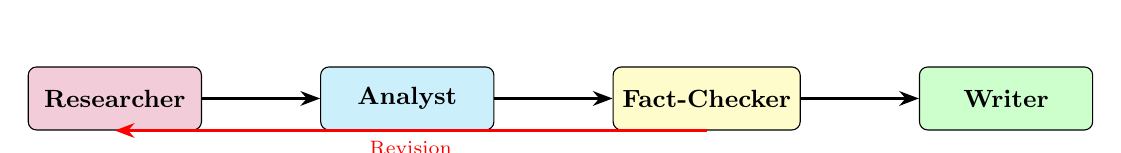
\begin{tikzpicture}[
    node distance=1.5cm,
    agent/.style={rectangle, draw, fill=blue!10, minimum width=2.2cm, minimum height=0.8cm, align=center, rounded corners=3pt, font=\small\bfseries},
    arrow/.style={-{Stealth[length=2.5mm]}, thick},
]
\node[agent, fill=purple!20] (r) {Researcher};
\node[agent, fill=cyan!20, right=of r] (a) {Analyst};
\node[agent, fill=yellow!20, right=of a] (f) {Fact-Checker};
\node[agent, fill=green!20, right=of f] (w) {Writer};
\draw[arrow] (r) -- (a);
\draw[arrow] (a) -- (f);
\draw[arrow] (f) -- (w);
\draw[arrow, red, bend right=30] (f.south) -- node[below, font=\scriptsize, red] {Revision} (r.south);
\end{tikzpicture}

\vfill
{\small Last Updated: August 2026}
\end{titlepage}

\tableofcontents
\newpage


% ═══════════════════════════════════════════════════════════════════════
% PART I: PROJECT OVERVIEW & ARCHITECTURE
% ═══════════════════════════════════════════════════════════════════════

\chapter{Project Ka Grand Overview --- Kahani Ki Shuruaat}

\begin{storybox}{Imagine karo ek research team...}
Socho tumhare paas ek research topic hai --- ``Quantum Computing ke latest breakthroughs kya hain?'' Ab agar tum akele ye research karo, toh kya karoge?
\begin{enumerate}
    \item Pehle Google pe search karoge (ya Tavily/DuckDuckGo)
    \item Results padhke notes banao
    \item Phir analyze karo --- kya themes hain, kya contradictions hain
    \item Facts verify karo --- kya sab sahi hai?
    \item Agar kuch galat mila toh phir se search karo
    \item Final mein ek polished report likho
\end{enumerate}

\textbf{Yehi kaam humara MARO system automatically karta hai --- but 4 specialized AI agents ke through!} Har agent ek expert hai apne kaam mein. Researcher search karta hai, Analyst analyze karta hai, Fact-Checker verify karta hai, aur Writer report likhta hai.
\end{storybox}

\section{MARO Kya Hai? --- One Line Definition}

\begin{conceptbox}{Core Definition}
\textbf{Multi-Agent Research Orchestrator (MARO)} ek full-stack AI-powered research platform hai jo \textbf{LangGraph StateGraph} use karke \textbf{4 autonomous AI agents} ko orchestrate karta hai --- jo kisi bhi topic pe web search + RAG retrieval se data collect karke, analyze karke, fact-check karke, aur ek publication-ready Markdown report generate karta hai --- with automatic revision loops jab fact-checker ko issues milte hain.
\end{conceptbox}

\begin{analogy}{Hospital ki Team}
MARO ko ek hospital ki team ki tarah samjho:
\begin{itemize}
    \item \textbf{Researcher = Lab Technician:} Tests conduct karta hai, data collect karta hai (web search + RAG)
    \item \textbf{Analyst = Senior Doctor:} Lab results dekh ke diagnosis karta hai (themes, contradictions)
    \item \textbf{Fact-Checker = Pathologist:} Har test result ko verify karta hai (claim verification)
    \item \textbf{Writer = Medical Report Writer:} Final medical report likhta hai (Markdown report)
    \item \textbf{Revision Loop = Second Opinion:} Agar pathologist ko doubt ho toh wapas tests karao
    \item \textbf{LangGraph = Hospital Management System:} Sabko coordinate karta hai
\end{itemize}
\end{analogy}

\section{Project Ke Key Differentiators}

Interview mein pehla question hoga: ``Is project mein kya special hai? Why not just ChatGPT se pooch lo?''

\begin{enumerate}[label=\textbf{\arabic*.}]
    \item \textbf{Multi-Agent Architecture:} Single LLM call nahi --- 4 specialized agents ka pipeline jahan har agent apne domain ka expert hai
    \item \textbf{Feedback Loop (Self-Correction):} Fact-Checker agar ``NEEDS\_REVISION'' bolta hai toh Researcher phir se search karta hai --- ye loop MAX\_REVISIONS tak chal sakta hai
    \item \textbf{RAG Integration:} Users apne PDFs upload kar sakte hain jo ChromaDB vector store mein index hote hain --- agents unhe bhi context mein use karte hain
    \item \textbf{Multi-Provider LLM:} Groq, Gemini, OpenAI, Anthropic, Ollama --- koi bhi provider use kar sakte ho, with automatic fallback
    \item \textbf{Full Stack:} React SPA frontend + Django REST backend + SSE real-time streaming
    \item \textbf{MCP Server:} FastMCP protocol se Claude Desktop ya Cursor IDE mein tools directly integrate ho jaate hain
    \item \textbf{Benchmark Arena:} Single-agent vs Multi-agent comparison with LLM-as-judge scoring
    \item \textbf{Multi-Format Export:} Markdown, HTML, JSON, BibTeX mein reports export
    \item \textbf{Research Memory:} System apni pichli research yaad rakhta hai aur future research mein use karta hai
    \item \textbf{62 Tests:} Comprehensive test suite with 100\% pass rate
\end{enumerate}

\begin{interviewbox}{Why Multi-Agent and not Single LLM?}
\textbf{Answer:} ``Sir, single LLM call mein ek model ko sab kuch karna padta hai --- search, analyze, verify, write. Isse do problems hain: pehla, hallucinations zyada hoti hain kyunki koi verification step nahi hai, aur doosra, depth kam hoti hai kyunki model har kaam mein ``jack of all trades, master of none'' ban jaata hai.

Humara multi-agent approach har kaam ko ek specialist agent ko deta hai. Researcher sirf search pe focused hai with Tavily API aur DuckDuckGo. Analyst sirf analysis pe focused hai --- themes, contradictions, consensus identify karta hai. Fact-Checker sirf verification pe focused hai --- har claim ko source data se match karta hai. Writer sirf report writing pe focused hai --- structured Markdown with citations.

Plus, agar Fact-Checker ko lagta hai ki research mein gaps hain ya claims unverified hain, toh woh Researcher ko wapas bhej deta hai improved queries ke saath --- ye revision loop quality ko significantly improve karta hai.

Humara benchmark arena actually empirically prove karta hai ki multi-agent reports better hain --- depth score aur verifiability score dono mein multi-agent consistently higher score karta hai vs single-agent baseline. Ye sirf theoretical argument nahi hai --- measured hai.''
\end{interviewbox}

\section{Technology Stack --- Complete Breakdown}

\begin{longtable}{|p{2.5cm}|p{3.5cm}|p{7cm}|}
\hline
\textbf{Layer} & \textbf{Technology} & \textbf{Purpose aur Kyun Choose Kiya} \\
\hline
\endhead
AI Core & LangGraph & StateGraph workflow engine --- conditional edges aur streaming support ke liye choose kiya \\
\hline
AI Core & LangChain & LLM abstraction --- ek interface, multiple providers ke liye \\
\hline
AI Core & ChromaDB & Lightweight vector DB --- SQLite backend, no external server needed \\
\hline
AI Core & HuggingFace & Sentence-transformers embeddings --- free, offline, fast \\
\hline
AI Core & Tavily API & Premium web search --- structured results aur high quality \\
\hline
AI Core & DuckDuckGo & Free fallback search --- no API key required \\
\hline
Backend & Django 5.1.x & Latest Python Web framework --- Async views, ORM, Admin, Migrations \\
\hline
Backend & DRF & REST API toolkit --- serializers, auth, throttling built-in \\
\hline
Backend & SQLite & Zero-config database --- single file, no server \\
\hline
Backend & CORS Headers & Cross-origin requests --- frontend alag port pe hai \\
\hline
Frontend & React 18 & Component-based UI --- efficient re-renders with virtual DOM \\
\hline
Frontend & Vite & Ultra-fast build tool --- HMR (Hot Module Replacement) in milliseconds \\
\hline
Frontend & Lucide React & Modern icon library --- consistent, lightweight SVG icons \\
\hline
Frontend & marked.js & Markdown parser --- research reports ko HTML mein render karna \\
\hline
Frontend & canvas-confetti & Celebration animation --- user delight on research completion \\
\hline
Integration & FastMCP & AI tool protocol --- Claude Desktop integration \\
\hline
Integration & Pydantic & Data validation --- MCP tool inputs validate karna \\
\hline
Integration & httpx & Async HTTP client --- MCP se Django API call karna \\
\hline
\end{longtable}

\begin{hindibox}{Technology Choices ke Peeche ka Logic}
Interviewer aksar poochte hain ``Ye technology kyun choose ki?'' --- hamesha reason batao:
\begin{itemize}
    \item \textbf{SQLite vs PostgreSQL:} SQLite isliye kyunki ye self-contained project hai --- single file database, no external server setup needed. Production mein PostgreSQL recommend karunga for concurrent access.
    \item \textbf{Vite vs Create React App:} Vite kyunki CRA deprecated ho raha hai aur Vite ka HMR 10-100x faster hai.
    \item \textbf{ChromaDB vs Pinecone:} ChromaDB kyunki free hai, local chalta hai, aur small-medium scale ke liye perfect hai. Pinecone cloud-hosted hai --- paid.
    \item \textbf{SSE vs WebSocket:} SSE kyunki humara data flow unidirectional hai (server $\rightarrow$ client). WebSocket bidirectional ke liye hota hai --- unnecessary complexity.
\end{itemize}
\end{hindibox}


\section{Architecture Diagrams}

\begin{figure}[H]
\centering
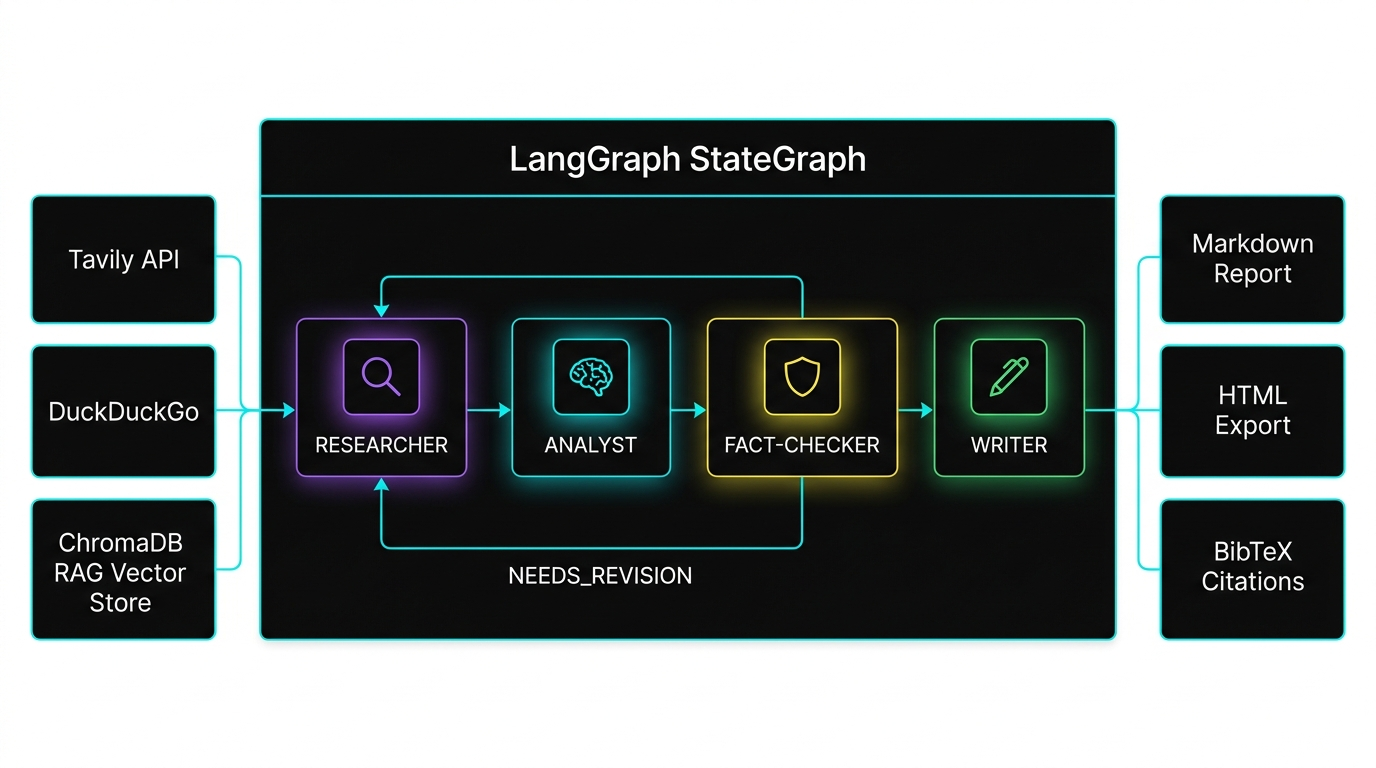
\includegraphics[width=\textwidth]{architecture_diagram.jpg}
\caption{MARO 4-Agent Pipeline Architecture --- LangGraph StateGraph ke through Researcher, Analyst, Fact-Checker, aur Writer agents ko orchestrate karta hai. Fact-Checker se Researcher ko feedback loop (NEEDS\_REVISION) dikhaya gaya hai. Left mein data sources (Tavily, DuckDuckGo, ChromaDB) aur right mein output formats (Markdown, HTML, BibTeX).}
\end{figure}

\begin{figure}[H]
\centering
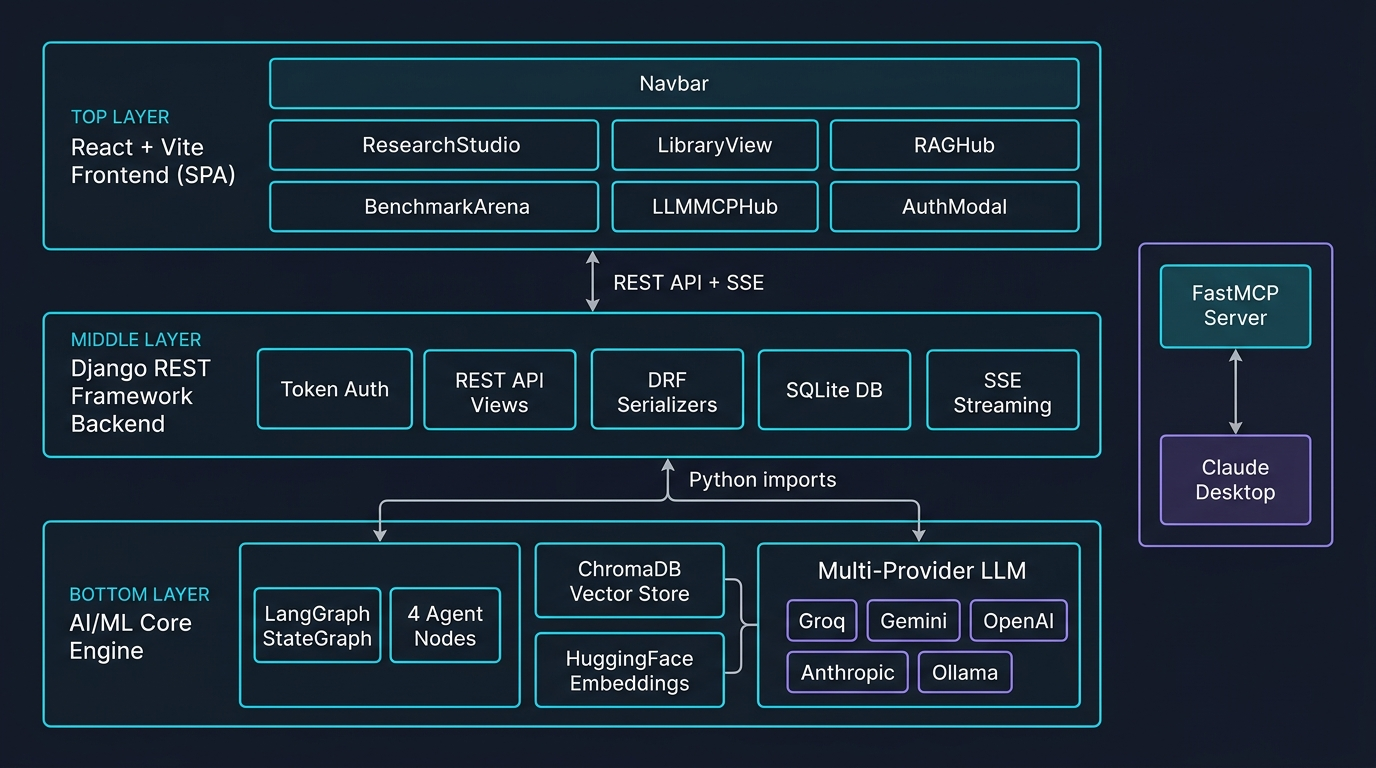
\includegraphics[width=\textwidth]{fullstack_architecture.jpg}
\caption{Full-Stack 3-Layer Architecture --- Top layer React+Vite Frontend (7 components), Middle layer Django REST Backend (Token Auth, REST API, SSE), Bottom layer AI/ML Core (LangGraph, 4 Agents, ChromaDB, Multi-Provider LLM). Side mein FastMCP Server Claude Desktop se connect hota hai.}
\end{figure}

\subsection{Architecture ko Interview Mein Kaise Explain Karein}

\begin{interviewbox}{Draw and explain the system architecture}
\textbf{Step-by-step whiteboard approach:}

\textbf{Step 1:} 3 boxes draw karo vertically --- ``Frontend'', ``Backend'', ``AI Core''

\textbf{Step 2:} Frontend box mein likho: ``React SPA --- ResearchStudio, Library, RAG Hub, Benchmarks''

\textbf{Step 3:} Arrows draw karo --- ``REST API (JSON)'' aur ``SSE (streaming)''

\textbf{Step 4:} Backend box mein: ``Django REST --- Token Auth, 18+ endpoints, SQLite''

\textbf{Step 5:} AI Core mein: ``LangGraph StateGraph --- 4 agents''

\textbf{Step 6:} 4 agents linear draw karo with feedback loop arrow

\textbf{Step 7:} Side mein: ``ChromaDB (RAG)'' aur ``Multi-Provider LLM''

\textbf{Step 8:} Explain karo: ``User topic deta hai, frontend Django ko POST karta hai, Django background thread mein LangGraph invoke karta hai, LangGraph 4 agents ko sequentially chalata hai, har agent events generate karta hai jo SSE se frontend tak stream hote hain, final report DB mein save hota hai.''
\end{interviewbox}


% ═══════════════════════════════════════════════════════════════════════
% CHAPTER 2: PROJECT STRUCTURE
% ═══════════════════════════════════════════════════════════════════════

\chapter{Project Structure --- Har File Ka Matlab Samjho}

\begin{storybox}{Project ko ek building ki tarah socho...}
Jaise ek building mein foundation, pillars, floors, aur roof hota hai --- waise hi humara project organized hai:
\begin{itemize}
    \item \textbf{Foundation (config/):} Settings, API keys, LLM providers --- building ka foundation
    \item \textbf{Blueprint (state/):} TypedDict schema --- building ka blueprint/naksha
    \item \textbf{Pillars (agents/):} 4 AI agents --- building ke main pillars jo kaam karte hain
    \item \textbf{Assembly Line (graph/):} LangGraph workflow --- agents ko connect karta hai
    \item \textbf{Library (rag/):} ChromaDB vector store --- building ki reference library
    \item \textbf{Reception (backend/):} Django REST API --- visitors (frontend) se baat karta hai
    \item \textbf{Showroom (frontend/):} React SPA --- visitors ko dikhta hai ye
    \item \textbf{Intercom (mcp\_server.py):} External AI tools se connect karta hai
    \item \textbf{Testing Lab (benchmark/):} Quality testing aur comparison
\end{itemize}
\end{storybox}

\section{Directory Tree with Detailed Explanation}

\begin{lstlisting}[style=pythonstyle,caption={Complete Project Structure --- Har File Ka Purpose},language={}]
Multi Agent Research Orchestrator/
|
|-- config/                      # CONFIGURATION LAYER
|   |-- __init__.py             # Re-exports: settings aur providers
|   |-- setting.py              # Environment variables aur constants
|   |                           # (MODEL_NAME, MAX_REVISIONS, CHUNK_SIZE)
|   |-- providers.py            # Multi-LLM provider abstraction
|                               # (Groq, Gemini, OpenAI, Anthropic, Ollama)
|
|-- state/                       # STATE SCHEMA LAYER
|   |-- schema.py               # ResearchState TypedDict
|                               # (shared memory between all agents)
|
|-- agents/                      # AI AGENT LAYER
|   |-- __init__.py
|   |-- researcher.py           # Agent 1: Web search + RAG retrieval
|   |                           # (Tavily/DDG + ChromaDB queries)
|   |-- analyst.py              # Agent 2: Analysis & theme synthesis
|   |                           # (Contradictions, consensus, gaps)
|   |-- fact_checker.py         # Agent 3: Claim verification
|   |                           # (PASSED/NEEDS_REVISION verdict)
|   |-- writer.py               # Agent 4: Report generation
|                               # (Markdown report + memory storage)
|
|-- graph/                       # WORKFLOW ORCHESTRATION LAYER
|   |-- workflow.py             # LangGraph StateGraph definition
|                               # (nodes, edges, conditional routing)
|
|-- rag/                         # RAG / VECTOR STORE LAYER
|   |-- vector_store.py         # ChromaDB operations
|                               # (ingest, search, store, stats)
|
|-- backend/                     # DJANGO REST API LAYER
|   |-- manage.py               # Django CLI entry point
|   |-- orchestrator_backend/   # Django project config
|   |   |-- settings.py         # Django settings (DB, auth, CORS)
|   |   |-- urls.py             # Root URL routing
|   |   |-- wsgi.py             # WSGI application
|   |-- api/                    # Django REST app
|       |-- models.py           # 5 DB models
|       |                       # (Session, Event, Source, Tag, Benchmark)
|       |-- serializers.py      # 8+ DRF serializers
|       |-- views.py            # 18+ API views
|       |-- services.py         # Business logic & job runner
|       |-- permissions.py      # Custom permission classes
|       |-- urls.py             # API URL patterns
|       |-- tests/              # 62 test cases
|           |-- conftest.py     # Pytest fixtures
|           |-- test_auth.py    # 14 auth tests
|           |-- test_research.py # 14 research tests
|           |-- test_benchmark.py # 10 benchmark tests
|
|-- frontend/                    # REACT SPA LAYER
|   |-- index.html              # Entry HTML
|   |-- vite.config.js          # Vite build configuration
|   |-- package.json            # NPM dependencies
|   |-- src/
|       |-- main.jsx            # React DOM mount point
|       |-- App.jsx             # Root component (tab routing)
|       |-- api.js              # Centralized API client
|       |-- index.css           # Global CSS design system
|       |-- components/         # UI Components
|           |-- ResearchStudio.jsx  # 861 lines - Main research UI
|           |-- AgentGraph.jsx      # Pipeline status visualizer
|           |-- LibraryView.jsx     # Session history & search
|           |-- RAGHubView.jsx      # Vector store management
|           |-- BenchmarkArenaView.jsx # A/B testing arena
|           |-- LLMMCPHubView.jsx   # Provider dashboard
|           |-- AuthModal.jsx       # Login/Register modal
|           |-- Navbar.jsx          # Navigation + system status
|
|-- benchmark/                   # BENCHMARK LAYER
|   |-- evaluator.py            # Single vs Multi comparison
|                               # (Heuristic + LLM-as-Judge scoring)
|
|-- mcp_server.py                # FastMCP Server (8 tools)
|-- requirements.txt             # Python dependencies
|-- Dockerfile                   # Container config
|-- docker-compose.yml           # Multi-container setup
|-- .env.example                 # Environment variable template
\end{lstlisting}

\begin{conceptbox}{Layered Architecture Pattern}
Project ko 6 layers mein organize kiya hai. Har layer sirf neeche wali layer pe depend karti hai, upar wali pe nahi:

\begin{center}
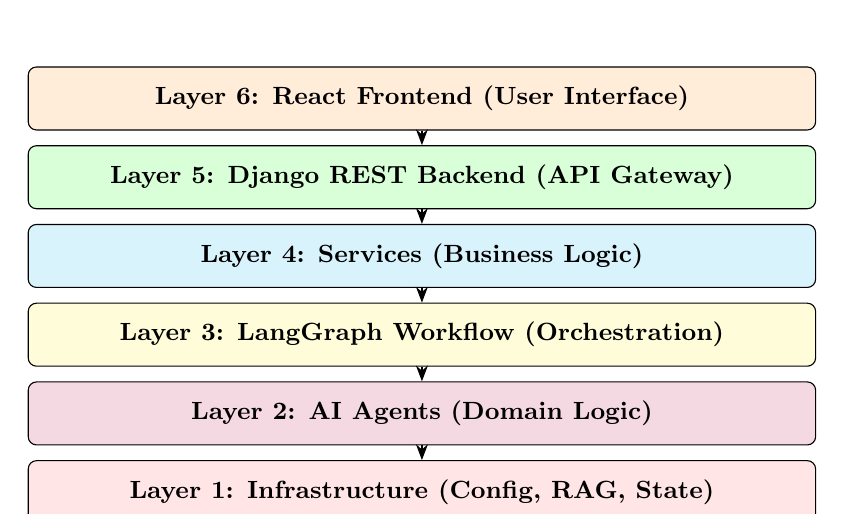
\begin{tikzpicture}[
    layer/.style={rectangle, draw, rounded corners=3pt, minimum width=10cm, minimum height=0.8cm, align=center, font=\small\bfseries},
    arrow/.style={-{Stealth[length=2mm]}, thick},
]
\node[layer, fill=orange!15] (frontend) at (0,5) {Layer 6: React Frontend (User Interface)};
\node[layer, fill=green!15] (backend) at (0,4) {Layer 5: Django REST Backend (API Gateway)};
\node[layer, fill=cyan!15] (services) at (0,3) {Layer 4: Services (Business Logic)};
\node[layer, fill=yellow!15] (graph) at (0,2) {Layer 3: LangGraph Workflow (Orchestration)};
\node[layer, fill=purple!15] (agents) at (0,1) {Layer 2: AI Agents (Domain Logic)};
\node[layer, fill=red!10] (infra) at (0,0) {Layer 1: Infrastructure (Config, RAG, State)};

\draw[arrow] (frontend) -- (backend);
\draw[arrow] (backend) -- (services);
\draw[arrow] (services) -- (graph);
\draw[arrow] (graph) -- (agents);
\draw[arrow] (agents) -- (infra);
\end{tikzpicture}
\end{center}

\textbf{Kyun Layered?} Separation of Concerns --- agar hum frontend ko React se Vue mein change karein, toh backend ko koi fark nahi padta. Agar hum ChromaDB ko Pinecone se replace karein, toh agents ko koi fark nahi padta. Har layer independently changeable hai.
\end{conceptbox}


% ═══════════════════════════════════════════════════════════════════════
% CHAPTER 3: STATE SCHEMA
% ═══════════════════════════════════════════════════════════════════════

\chapter{State Schema --- Agents Ki Shared Memory}

\begin{storybox}{Agents ek dusre se kaise baat karte hain?}
Imagine karo 4 log ek whiteboard ke around baithe hain. Har koi whiteboard pe kuch likhta hai aur doosra padh ke apna kaam karta hai. Ye whiteboard hai humara \textbf{ResearchState} --- ek shared dictionary jo sabke beech pass hoti hai. Koi direct messaging nahi hai agents ke beech --- sab kuch state ke through hota hai.

\textbf{Ye bahut important design decision hai:}
\begin{itemize}
    \item Agents decoupled hain --- ek agent doosre ko directly call nahi karta
    \item State ek ``contract'' hai --- sabko pata hai kya padhna hai aur kya likhna hai
    \item Testing easy hai --- mock state bana ke koi bhi agent independently test ho sakta hai
\end{itemize}
\end{storybox}

\section{ResearchState TypedDict --- Line by Line Explanation}

\begin{codewalkbox}{state/schema.py --- Complete Source Code}
\begin{lstlisting}[style=pythonstyle]
from __future__ import annotations
import operator
from typing import Annotated, TypedDict

class ResearchState(TypedDict):
    # ---- INPUT FIELD ----
    topic: str
    # User ka research topic, e.g., "quantum computing advances"
    # Ye field sirf ek baar set hota hai - START pe

    # ---- ACCUMULATOR FIELDS (Reducer: operator.add) ----
    research_data: Annotated[list[str], operator.add]
    # Researcher ke web search results
    # Har item format: "[Source: URL]\nContent..."
    # ACCUMULATES: revision pe purane results preserve hote hain

    rag_context: Annotated[list[str], operator.add]
    # ChromaDB se retrieved document chunks
    # Dono collections se: research_docs + past_research
    # ACCUMULATES: multiple retrievals combine hote hain

    # ---- REPLACE FIELDS (Latest value overwrites) ----
    analysis: str
    # Analyst ka structured analysis output
    # Format: Key Themes, Contradictions, Consensus, Gaps

    fact_check_result: str
    # Fact-checker ka detailed verification report
    # Har claim ke liye: VERIFIED/UNVERIFIED/CONTRADICTED

    fact_check_passed: bool
    # Simple boolean: True = quality OK, False = needs revision
    # Conditional edge isko check karta hai

    revision_count: int
    # Counter: kitni baar revision loop chala
    # 0 = first pass, 1 = after first revision, etc.

    final_report: str
    # Writer ka publication-ready Markdown report
    # Sirf last step mein set hota hai

    # ---- METADATA FIELDS ----
    messages: Annotated[list[str], operator.add]
    # Log messages from all agents
    # SSE streaming terminal mein dikhte hain
    # ACCUMULATES: har agent ke messages append hote hain

    current_agent: str
    # Currently active agent ka naam
    # UI mein pipeline visualizer isse use karta hai

    error: str
    # Error message agar koi exception aaye
    # Empty string = no error
\end{lstlisting}
\end{codewalkbox}

\subsection{TypedDict Deep Dive}

\begin{conceptbox}{TypedDict Kya Hai aur Kyun Use Kiya?}
Python mein normally dictionary ko koi bhi key de sakte ho:
\begin{lstlisting}[style=pythonstyle]
# Normal dict - koi bhi key chalti hai
state = {}
state["topik"] = "quantum"      # Typo! But no error
state["analysis"] = 42           # Wrong type! But no error
state["random_key"] = "anything" # Extra key! But no error
\end{lstlisting}

\textbf{TypedDict} se compile-time pe pata hota hai ki kaunsi keys hongi aur type kya hoga:
\begin{lstlisting}[style=pythonstyle]
# TypedDict - strictly typed
class ResearchState(TypedDict):
    topic: str           # Must be string
    analysis: str        # Must be string
    revision_count: int  # Must be integer

state: ResearchState = {
    "topik": "quantum",  # IDE warns: "topik" not in TypedDict
    "analysis": 42,      # IDE warns: expected str, got int
}
\end{lstlisting}

\textbf{Benefits:}
\begin{enumerate}
    \item IDE autocomplete milta hai --- \texttt{state["r..."} type karo aur \texttt{research\_data} suggest hoga
    \item Type checker (mypy) errors catch karta hai before runtime
    \item Documentation ka kaam bhi karta hai --- TypedDict padhke pata chal jaata hai ki state mein kya hai
    \item LangGraph ko state structure pata hota hai --- wo proper node outputs validate kar sakta hai
\end{enumerate}
\end{conceptbox}

\subsection{Annotated + operator.add --- The Reducer Pattern}

Ye MARO ka \textbf{sabse important concept} hai interview ke liye. Isko pakka samjh lo.

\begin{conceptbox}{LangGraph Reducer Pattern --- Deep Explanation}
\textbf{Problem:} LangGraph mein jab ek agent state return karta hai, toh default behavior hai ki purani value \textbf{replace} ho jaaye nayi se.

\textbf{Example without reducer:}
\begin{lstlisting}[style=pythonstyle]
# Iteration 1: Researcher returns
state["research_data"] = ["result1", "result2", "result3"]

# Iteration 2 (revision): Researcher returns again
state["research_data"] = ["result4", "result5"]
# PROBLEM: result1, result2, result3 LOST!
\end{lstlisting}

\textbf{Solution with reducer:}
\begin{lstlisting}[style=pythonstyle]
research_data: Annotated[list[str], operator.add]
# operator.add = list concatenation reducer

# Iteration 1: Researcher returns ["result1", "result2", "result3"]
# State: ["result1", "result2", "result3"]

# Iteration 2 (revision): Researcher returns ["result4", "result5"]
# State: ["result1", "result2", "result3", "result4", "result5"]
# ALL results preserved!
\end{lstlisting}

\textbf{How it works internally:}
\begin{lstlisting}[style=pythonstyle]
# LangGraph internal logic (simplified):
def update_state(old_state, agent_output):
    for key, new_value in agent_output.items():
        if has_reducer(key):
            reducer_fn = get_reducer(key)  # operator.add
            old_state[key] = reducer_fn(old_state[key], new_value)
            # list.__add__([old], [new]) = [old] + [new]
        else:
            old_state[key] = new_value  # Simple replace
\end{lstlisting}
\end{conceptbox}

\begin{hindibox}{Reducer Pattern ko Simple Hindi mein Samjho}
Socho tumhare paas ek shopping list hai.

\textbf{Bina Reducer (Replace):} Har baar jab tum market jaate ho, purani list phad ke nayi likho. Toh pehle ke items yaad nahi rahenge.

\textbf{Reducer ke saath (Accumulate):} Har baar jab tum market jaate ho, naye items purani list ke neeche add karo. Toh saari history preserved rehti hai.

Humara \texttt{research\_data} field aise hi kaam karta hai --- har revision mein naye search results purane ke saath add hote hain. \texttt{analysis} field replace hota hai kyunki hum always latest analysis chahte hain.
\end{hindibox}

\subsection{Har Field Ka Detailed Purpose}

\begin{longtable}{|p{3cm}|p{2cm}|p{1.5cm}|p{2cm}|p{4.5cm}|}
\hline
\textbf{Field} & \textbf{Type} & \textbf{Reducer?} & \textbf{Who Writes} & \textbf{Detailed Explanation} \\
\hline
\endhead
\texttt{topic} & \texttt{str} & No & User & User ne kya research topic diya. Set hota hai initial state mein, agents modify nahi karte. \\
\hline
\texttt{research\_data} & \texttt{list[str]} & Yes (add) & Researcher & Web search results. Har item mein source URL + content hota hai. Revision pe accumulate. \\
\hline
\texttt{rag\_context} & \texttt{list[str]} & Yes (add) & Researcher & ChromaDB se retrieved chunks. research\_docs (uploaded PDFs) + past\_research (memory). \\
\hline
\texttt{analysis} & \texttt{str} & No & Analyst & Structured analysis with themes, contradictions, consensus, gaps. Latest analysis hi relevant. \\
\hline
\texttt{fact\_check\_result} & \texttt{str} & No & Fact-Checker & Detailed report --- har claim VERIFIED/UNVERIFIED with source evidence. \\
\hline
\texttt{fact\_check\_passed} & \texttt{bool} & No & Fact-Checker & Simple gate: True = proceed to Writer, False = go back to Researcher. \\
\hline
\texttt{revision\_count} & \texttt{int} & No & Fact-Checker & Increments when revision happens. Guards against infinite loops (max 2). \\
\hline
\texttt{final\_report} & \texttt{str} & No & Writer & Publication-ready Markdown report. Only set at the very end. \\
\hline
\texttt{messages} & \texttt{list[str]} & Yes (add) & All Agents & Log messages. SSE streaming terminal mein real-time dikhte hain. \\
\hline
\texttt{current\_agent} & \texttt{str} & No & All Agents & Active agent name. Frontend pipeline visualizer isse highlight karta hai. \\
\hline
\texttt{error} & \texttt{str} & No & Any Agent & Error message. Empty = no error. Non-empty = something went wrong. \\
\hline
\end{longtable}

\begin{interviewbox}{Explain the state management in your multi-agent system}
\textbf{Answer:} ``Maine LangGraph ka TypedDict-based state management use kiya hai. \texttt{ResearchState} ek shared typed dictionary hai jo sab agents ke beech pass hoti hai. Isme 11 fields hain jo 3 categories mein aate hain:

\textbf{Accumulator fields} (\texttt{research\_data}, \texttt{rag\_context}, \texttt{messages}) --- inme \texttt{Annotated[list, operator.add]} reducer hai, matlab data append hota hai, replace nahi. Ye critical hai revision loop ke liye --- jab Researcher dubara search karta hai, naye results purane ke saath merge hote hain.

\textbf{Replace fields} (\texttt{analysis}, \texttt{fact\_check\_result}, \texttt{final\_report}) --- inme latest value hi relevant hai, toh default replace behavior use hota hai.

\textbf{Control flow fields} (\texttt{fact\_check\_passed}, \texttt{revision\_count}) --- ye conditional routing control karte hain. \texttt{should\_continue()} function \texttt{fact\_check\_passed} check karta hai aur decide karta hai ki Writer pe jaana hai ya Researcher pe wapas.

TypedDict use karne ka benefit ye hai ki IDE autocomplete deta hai, type checker errors early catch karta hai, aur documentation ka bhi kaam karta hai.''
\end{interviewbox}


% ═══════════════════════════════════════════════════════════════════════
% CHAPTER 4: CONFIGURATION LAYER
% ═══════════════════════════════════════════════════════════════════════

\chapter{Configuration Layer --- Settings aur Multi-Provider LLM}

\section{config/setting.py --- Environment Variables Management}

\begin{storybox}{Sensitive data kahan rakhte hain?}
API keys, model names, database paths --- ye sab code mein hardcode nahi karte. Imagine karo tumne Groq API key directly Python file mein likh di:

\texttt{GROQ\_API\_KEY = "gsk\_abc123secret"}

Ab ye file GitHub pe push ho gayi --- duniya ko tumhari API key mil gayi! Koi bhi tumhara quota use kar sakta hai. Isliye \texttt{.env} file mein rakhte hain jo \texttt{.gitignore} mein hoti hai.
\end{storybox}

\begin{codewalkbox}{config/setting.py --- Smart Configuration Loader}
\begin{lstlisting}[style=pythonstyle]
import os
from dotenv import load_dotenv

load_dotenv()
# ^^ .env file ko OS environment mein load karta hai
# .env file format:
#   GROQ_API_KEY=gsk_abc123
#   MODEL_NAME=llama-3.3-70b-versatile
#   MAX_REVISIONS=2

def get_env_var(key, default=None, required=False):
    """Smart environment variable loader with 3-source fallback"""

    # SOURCE 1: OS Environment Variables
    value = os.getenv(key)
    # Docker, Render, Vercel -> env vars yahan se aate hain

    if not value:
        try:
            # SOURCE 2: Streamlit Secrets
            import streamlit as st
            if key in st.secrets:
                value = str(st.secrets[key])
            # Streamlit Cloud deployment -> secrets.toml se aate hain
        except Exception:
            pass  # Streamlit not installed? Skip silently

    if not value:
        # SOURCE 3: Default Value
        value = default
        # Fallback for local development without .env

    if required and not value:
        raise ValueError(f"Required environment variable missing: {key}")

    return value or ""
\end{lstlisting}
\end{codewalkbox}

\begin{conceptbox}{Triple-Source Configuration Pattern}
\texttt{get\_env\_var()} 3 sources se values load karta hai priority order mein:

\begin{center}
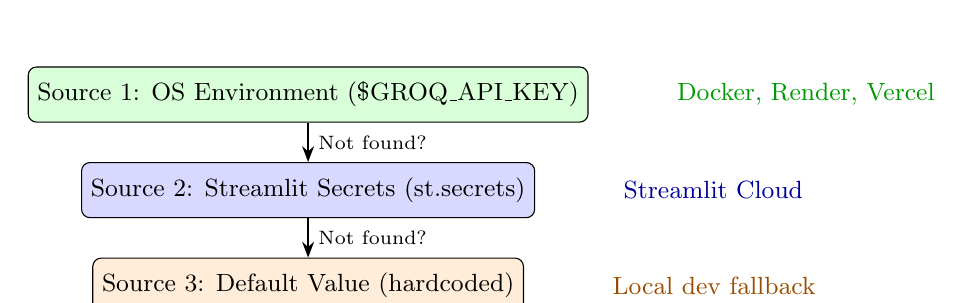
\begin{tikzpicture}[
    node distance=0.5cm,
    box/.style={rectangle, draw, rounded corners=3pt, minimum width=5cm, minimum height=0.7cm, align=center, font=\small},
    arrow/.style={-{Stealth[length=2mm]}, thick},
]
\node[box, fill=green!15] (os) {Source 1: OS Environment (\$GROQ\_API\_KEY)};
\node[box, fill=blue!15, below=of os] (st) {Source 2: Streamlit Secrets (st.secrets)};
\node[box, fill=orange!15, below=of st] (def) {Source 3: Default Value (hardcoded)};

\node[right=1cm of os, font=\small\color{green!60!black}] {Docker, Render, Vercel};
\node[right=1cm of st, font=\small\color{blue!60!black}] {Streamlit Cloud};
\node[right=1cm of def, font=\small\color{orange!60!black}] {Local dev fallback};

\draw[arrow] (os) -- node[right, font=\scriptsize] {Not found?} (st);
\draw[arrow] (st) -- node[right, font=\scriptsize] {Not found?} (def);
\end{tikzpicture}
\end{center}
\end{conceptbox}

\subsection{All Configuration Constants}

\begin{lstlisting}[style=pythonstyle,caption={config/setting.py --- All Constants}]
# === API KEYS ===
GROQ_API_KEY = get_env_var("GROQ_API_KEY")
TAVILY_API_KEY = get_env_var("TAVILY_API_KEY")
OPENAI_API_KEY = get_env_var("OPENAI_API_KEY")
ANTHROPIC_API_KEY = get_env_var("ANTHROPIC_API_KEY")
GEMINI_API_KEY = get_env_var("GEMINI_API_KEY")

# === LLM CONFIGURATION ===
MODEL_NAME = get_env_var("MODEL_NAME",
    default="llama-3.3-70b-versatile")
# ^^ Groq ke liye default model
# Ye per-provider override hota hai providers.py mein

MAX_SEARCH_RESULTS = int(get_env_var("MAX_SEARCH_RESULTS",
    default="5"))
# ^^ Har search query se kitne results lene hain
# 5 = balanced (zyada results = better coverage but slower)

MAX_REVISIONS = int(get_env_var("MAX_REVISIONS",
    default="2"))
# ^^ Feedback loop kitni baar chal sakta hai maximum
# 2 = default (0 = first pass, 1 = after revision 1, 2 = after revision 2)

# === RAG / CHROMADB CONFIGURATION ===
CHROMA_PERSIST_DIR = get_env_var("CHROMA_PERSIST_DIR",
    default="./chroma_db")
# ^^ ChromaDB data directory --- persistent storage

EMBEDDING_MODEL = get_env_var("EMBEDDING_MODEL",
    default="sentence-transformers/all-MiniLM-L6-v2")
# ^^ HuggingFace embedding model
# all-MiniLM-L6-v2: 384 dimensions, fast, good quality

CHUNK_SIZE = int(get_env_var("CHUNK_SIZE", default="1000"))
# ^^ PDF chunk size in characters
# 1000 = ~250 words per chunk

CHUNK_OVERLAP = int(get_env_var("CHUNK_OVERLAP", default="200"))
# ^^ Adjacent chunks mein overlap
# 200 chars = ~50 words overlap for context continuity
\end{lstlisting}

\begin{interviewbox}{How do you manage configuration across environments?}
\textbf{Answer:} ``Centralized configuration module hai \texttt{config/setting.py} mein. Ek smart \texttt{get\_env\_var()} function hai jo 3 sources se priority order mein values load karta hai: pehle OS environment variables (Docker/production/Render ke liye), phir Streamlit Secrets (Streamlit Cloud deployment ke liye), aur last mein hardcoded default values (local development ke liye). API keys kabhi source code mein nahi hain --- sab \texttt{.env} file se aate hain jo \texttt{.gitignore} mein hai. Constants jaise \texttt{MAX\_REVISIONS=2}, \texttt{CHUNK\_SIZE=1000}, \texttt{MAX\_SEARCH\_RESULTS=5} sab environment se tunable hain bina code change kiye. Ye 12-factor app methodology follow karta hai jahan config environment mein rakhte hain, code mein nahi.''
\end{interviewbox}

\section{config/providers.py --- Multi-Provider LLM Abstraction}

Ye file project ka ek ``secret weapon'' hai. Ye ek single function \texttt{get\_llm\_with\_fallback()} provide karti hai jo automatically best available LLM provider select karke LangChain ChatModel return karti hai.

\begin{analogy}{Restaurant ke Multiple Chefs}
Socho ek restaurant hai jahan 5 chefs hain:
\begin{itemize}
    \item \textbf{Chef Groq:} Ultra-fast (500 tokens/sec), but sometimes busy
    \item \textbf{Chef Gemini:} Google ka, balanced speed aur quality
    \item \textbf{Chef OpenAI:} GPT-4o, very smart but expensive
    \item \textbf{Chef Anthropic:} Claude, precise analytical writing
    \item \textbf{Chef Ollama:} Local kitchen, no internet needed, always available
\end{itemize}
Manager pehle sabse fast available chef ko bhejta hai. Agar woh busy hai (API key nahi / rate limited), toh doosre ko try karta hai.
\end{analogy}

\subsection{Provider Priority Chain}

\begin{lstlisting}[style=pythonstyle]
PROVIDER_PRIORITY = ["groq", "gemini", "openai", "anthropic", "ollama"]

_KEY_ENV = {
    "groq": "GROQ_API_KEY",
    "gemini": "GEMINI_API_KEY",       # Also checks GOOGLE_API_KEY
    "openai": "OPENAI_API_KEY",
    "anthropic": "ANTHROPIC_API_KEY",
    "ollama": None,                    # No key needed (local)
}

_DEFAULT_MODELS = {
    "groq": "llama-3.3-70b-versatile",  # 70B params, very capable
    "gemini": "gemini-2.0-flash",        # Google's latest flash model
    "openai": "gpt-4o",                  # GPT-4 Omni
    "anthropic": "claude-sonnet-4-20250514",  # Claude Sonnet 4
    "ollama": "llama3.1",                # Local Llama 3.1
}
\end{lstlisting}

\subsection{Auto-Detection Logic --- How Provider is Selected}

\begin{lstlisting}[style=pythonstyle]
def _detect() -> str:
    """Detect which LLM provider to use"""

    # Step 1: User ne explicitly provider set kiya?
    requested = _env("LLM_PROVIDER", "auto").lower()
    if requested in PROVIDER_PRIORITY:
        return requested
        # e.g., LLM_PROVIDER=openai -> directly use OpenAI

    # Step 2: Auto mode - check which providers have API keys
    for p in PROVIDER_PRIORITY:
        if _has_key(p):
            return p
    # Priority order: groq > gemini > openai > anthropic > ollama

    # Step 3: Ultimate fallback - Ollama (no key needed)
    return "ollama"
\end{lstlisting}

\begin{conceptbox}{Provider Detection Flow Diagram}
\begin{center}
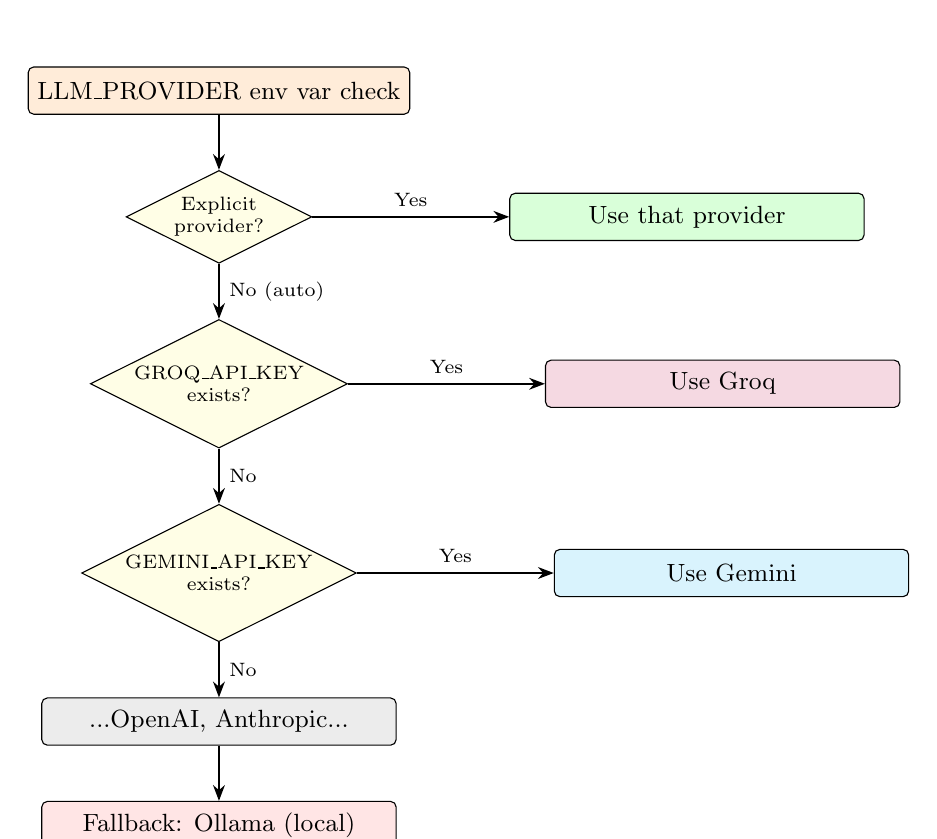
\begin{tikzpicture}[
    node distance=0.7cm,
    box/.style={rectangle, draw, rounded corners=2pt, minimum width=4.5cm, minimum height=0.6cm, align=center, font=\small},
    decision/.style={diamond, draw, aspect=2, minimum width=1.5cm, align=center, font=\scriptsize, inner sep=1pt},
    arrow/.style={-{Stealth[length=2mm]}, thick},
]

\node[box, fill=orange!15] (start) {LLM\_PROVIDER env var check};
\node[decision, fill=yellow!10, below=of start] (d1) {Explicit\\provider?};
\node[box, fill=green!15, right=2.5cm of d1] (use) {Use that provider};
\node[decision, fill=yellow!10, below=of d1] (d2) {GROQ\_API\_KEY\\exists?};
\node[box, fill=purple!15, right=2.5cm of d2] (groq) {Use Groq};
\node[decision, fill=yellow!10, below=of d2] (d3) {GEMINI\_API\_KEY\\exists?};
\node[box, fill=cyan!15, right=2.5cm of d3] (gemini) {Use Gemini};
\node[box, fill=gray!15, below=of d3] (more) {...OpenAI, Anthropic...};
\node[box, fill=red!10, below=of more] (ollama) {Fallback: Ollama (local)};

\draw[arrow] (start) -- (d1);
\draw[arrow] (d1) -- node[above, font=\scriptsize] {Yes} (use);
\draw[arrow] (d1) -- node[right, font=\scriptsize] {No (auto)} (d2);
\draw[arrow] (d2) -- node[above, font=\scriptsize] {Yes} (groq);
\draw[arrow] (d2) -- node[right, font=\scriptsize] {No} (d3);
\draw[arrow] (d3) -- node[above, font=\scriptsize] {Yes} (gemini);
\draw[arrow] (d3) -- node[right, font=\scriptsize] {No} (more);
\draw[arrow] (more) -- (ollama);
\end{tikzpicture}
\end{center}
\end{conceptbox}

\subsection{get\_llm\_with\_fallback() --- The Resilient LLM Loader}

\begin{lstlisting}[style=pythonstyle,caption={The most critical function in providers.py}]
def get_llm_with_fallback(model=None, temperature=0.3):
    """
    Try active provider first, then fallback through others.

    Args:
        model: Specific model name (None = use per-provider default)
        temperature: Creativity level (0.0 = deterministic,
                                       1.0 = very creative)

    Returns:
        LangChain ChatModel instance

    Raises:
        RuntimeError: If ALL providers fail
    """
    active = _detect()  # Best available provider
    # Try order: active first, then rest of priority chain
    to_try = [active] + [p for p in PROVIDER_PRIORITY if p != active]
    last_error = None

    for p in to_try:
        if not _has_key(p):
            continue  # Skip providers without API keys

        try:
            # Model selection: explicit > env var > per-provider default
            m = model or _env("MODEL_NAME", "") or _DEFAULT_MODELS[p]

            if p == "groq":
                from langchain_groq import ChatGroq
                # ^^ LAZY IMPORT! Inside loop, not at top of file
                return ChatGroq(
                    model=m,
                    temperature=temperature,
                    groq_api_key=_env("GROQ_API_KEY"),
                )

            elif p == "gemini":
                from langchain_google_genai import ChatGoogleGenerativeAI
                api_key = _env("GEMINI_API_KEY") or _env("GOOGLE_API_KEY")
                return ChatGoogleGenerativeAI(
                    model=m,
                    temperature=temperature,
                    google_api_key=api_key,
                )

            elif p == "openai":
                from langchain_openai import ChatOpenAI
                return ChatOpenAI(
                    model=m,
                    temperature=temperature,
                    openai_api_key=_env("OPENAI_API_KEY"),
                )

            elif p == "anthropic":
                from langchain_anthropic import ChatAnthropic
                return ChatAnthropic(
                    model=m,
                    temperature=temperature,
                    anthropic_api_key=_env("ANTHROPIC_API_KEY"),
                )

            elif p == "ollama":
                from langchain_ollama import ChatOllama
                return ChatOllama(
                    model=m,
                    temperature=temperature,
                    base_url=_env("OLLAMA_BASE_URL",
                                "http://localhost:11434"),
                )

        except Exception as exc:
            last_error = exc
            logger.warning("Provider %s failed: %s", p, exc)
            # Don't crash! Try next provider...

    # ALL providers failed
    raise RuntimeError(
        f"No LLM provider available. Last error: {last_error}"
    ) from last_error
\end{lstlisting}

\begin{warningbox}{Lazy Imports --- Ye Kyun Zaroori Hai?}
\texttt{from langchain\_groq import ChatGroq} ko function ke andar, loop ke andar likha hai --- top of file pe nahi. Ye \textbf{intentional design decision} hai:

\textbf{Problem:} Agar sab imports top pe hon:
\begin{lstlisting}[style=pythonstyle]
from langchain_groq import ChatGroq        # OK
from langchain_openai import ChatOpenAI    # OK
from langchain_anthropic import ChatAnthropic  # ImportError!
# User ne pip install langchain-anthropic nahi kiya
# ENTIRE MODULE CRASHES! Groq bhi use nahi ho paayega.
\end{lstlisting}

\textbf{Solution:} Lazy imports --- sirf woh import karo jo actually use ho raha hai:
\begin{lstlisting}[style=pythonstyle]
if p == "groq":
    from langchain_groq import ChatGroq  # Only if needed
    return ChatGroq(...)
elif p == "anthropic":
    from langchain_anthropic import ChatAnthropic  # Only if needed
    return ChatAnthropic(...)
# Anthropic not installed? No problem!
# Loop skips to next provider.
\end{lstlisting}

\textbf{Benefit:} User ko sirf apne preferred provider ka package install karna padega, baaki sab optional hain.
\end{warningbox}

\begin{interviewbox}{How does your multi-provider LLM system work?}
\textbf{Answer:} ``Provider abstraction layer hai \texttt{config/providers.py} mein. 5 providers support hain: Groq (ultra-fast inference on LPUs), Gemini (Google ka large context model), OpenAI (GPT-4o), Anthropic (Claude Sonnet 4), aur Ollama (local, no cloud dependency).

\texttt{get\_llm\_with\_fallback()} function pehle active provider detect karta hai based on available API keys (priority: Groq $>$ Gemini $>$ OpenAI $>$ Anthropic $>$ Ollama). Phir us provider se ChatModel create karne ki try karta hai. Agar fail ho --- network error, invalid key, rate limit --- toh next priority provider pe automatically fall through karta hai.

Key design decisions: (1) Lazy imports --- \texttt{from langchain\_groq import ChatGroq} loop ke andar hai, toh agar koi provider package installed nahi hai toh ImportError nahi aata, sirf skip hota hai. (2) Per-provider default models --- Groq ke liye llama-3.3-70b, Gemini ke liye gemini-2.0-flash, etc. (3) Agents \texttt{model=None} pass karte hain toh automatic per-provider default use hota hai. (4) Ollama ko API key nahi chahiye, toh ye always available hai as ultimate fallback for offline use.

Ye Strategy Pattern hai with Chain of Responsibility fallback.''
\end{interviewbox}


% ═══════════════════════════════════════════════════════════════════════
% CHAPTER 5: AI AGENTS IN DEPTH
% ═══════════════════════════════════════════════════════════════════════

\chapter{AI Agents --- MARO Ka Dimaag (In-Depth)}

\section{Agent Design Philosophy}

\begin{conceptbox}{Agent Design Pattern --- Universal Template}
MARO mein har agent ek pure function hai jo ye pattern follow karta hai:

\begin{lstlisting}[style=pythonstyle]
def agent_node(state: ResearchState) -> dict:
    """Universal agent template"""
    # Step 1: Read relevant fields from state
    topic = state["topic"]
    relevant_data = state.get("some_field", default)

    # Step 2: Get LLM instance
    llm = get_llm_with_fallback(model=None, temperature=0.3)

    # Step 3: Construct prompt with context
    prompt = SYSTEM_PROMPT.format(topic=topic, data=relevant_data)

    # Step 4: Invoke LLM
    try:
        response = llm.invoke([
            SystemMessage(content=prompt),
            HumanMessage(content=f"Process: {topic}"),
        ])
        result = response.content
    except Exception as e:
        result = f"Fallback: {e}"  # Graceful degradation

    # Step 5: Return ONLY the fields this agent modifies
    return {
        "output_field": result,
        "messages": [f"Agent completed: {summary}"],
        "current_agent": "agent_name",
    }
\end{lstlisting}

\textbf{Important:} Agent ko poori state milti hai but woh sirf relevant fields read karta hai aur sirf apne output fields return karta hai. Ye \textbf{Separation of Concerns} hai.
\end{conceptbox}

\begin{analogy}{Assembly Line Workers}
Ek car factory mein:
\begin{itemize}
    \item Worker 1 (Researcher): Raw materials laata hai (steel, rubber, glass)
    \item Worker 2 (Analyst): Materials ki quality check karta hai, sort karta hai
    \item Worker 3 (Fact-Checker): Final inspection --- sab specs meet ho rahe hain?
    \item Worker 4 (Writer): Car ko polish karke delivery ready karta hai
\end{itemize}
Har worker apni station pe kaam karta hai. Worker 1 ko nahi pata Worker 4 kya karega. Sab ek conveyor belt (state) ke through connected hain. Agar Inspector (Fact-Checker) ko defect mile toh conveyor belt wapas jaata hai.
\end{analogy}

\section{Agent 1: Researcher --- The Evidence Gatherer}

\begin{storybox}{Researcher Agent ki kahani}
Researcher ek detective hai jo crime scene pe evidence collect karta hai. Uska kaam hai maximum relevant information gather karna. Woh smart hai --- pehle topic ke 3 alag angles se search queries banata hai (query diversification), phir 2 search engines use karta hai (Tavily primary, DuckDuckGo fallback), aur ChromaDB se past documents bhi check karta hai. Agar ye revision loop hai (fact-checker ne wapas bheja), toh researcher purane queries nahi daalta --- fact-checker ke feedback ke basis pe naye, improved queries generate karta hai.
\end{storybox}

\subsection{System Prompts --- LLM Ko Role Batana}

\begin{lstlisting}[style=pythonstyle,caption={Researcher Prompts}]
QUERY_GEN_PROMPT = """You are a research query strategist.
Given a research topic, generate exactly 3 diverse, specific
search queries that will cover different angles of the topic.

REQUIREMENTS:
- Each query should explore a DIFFERENT aspect
- Be specific enough to get targeted results
- Include temporal qualifiers where appropriate
- Return ONLY the 3 queries, one per line, no numbering

Example for "AI in Healthcare":
  - "artificial intelligence diagnostic imaging FDA approved 2024"
  - "machine learning drug discovery clinical trials results"
  - "AI patient data privacy HIPAA compliance challenges"
"""

REVISION_PROMPT = """You are a research query strategist.
The fact-checker flagged issues with previous research.
Based on the feedback below, generate 3 NEW, improved
search queries that address the specific gaps and inaccuracies
identified. Do NOT repeat previous queries.

FACT-CHECKER FEEDBACK:
{feedback}"""
\end{lstlisting}

\begin{hindibox}{Prompt Engineering Techniques}
Humne researcher ke prompts mein kaafi techniques use ki hain:
\begin{enumerate}
    \item \textbf{Role Assignment:} ``You are a research query strategist'' --- LLM ko specific role dena
    \item \textbf{Exact Output Format:} ``Return ONLY the 3 queries, one per line'' --- format specify karna
    \item \textbf{Few-Shot Example:} ``Example for AI in Healthcare...'' --- ek example dena taaki LLM samjhe
    \item \textbf{Negative Instructions:} ``Do NOT repeat previous queries'' --- kya na kare ye bhi batana
    \item \textbf{Context Injection:} \texttt{\{feedback\}} --- runtime pe actual fact-checker feedback inject karna
\end{enumerate}
\end{hindibox}

\subsection{Query Generation --- Smart Search Strategy}

\begin{lstlisting}[style=pythonstyle,caption={researcher.py --- Query Generation Logic}]
def researcher_node(state: ResearchState) -> dict:
    topic = state["topic"]
    revision_count = state.get("revision_count", 0)
    sub_queries = [topic]  # Fallback: topic itself as query

    try:
        llm = get_llm_with_fallback(model=None, temperature=0.4)
        # temperature=0.4 for queries (slightly creative)

        # REVISION MODE: Use fact-checker's feedback
        if revision_count > 0 and state.get("fact_check_result"):
            prompt = REVISION_PROMPT.format(
                feedback=state["fact_check_result"]
            )
            # Researcher READS fact-checker's critique
            # and generates TARGETED queries to fix gaps
        else:
            # FIRST PASS: Generate diverse queries
            prompt = QUERY_GEN_PROMPT

        query_response = llm.invoke([
            SystemMessage(content=prompt),
            HumanMessage(content=f"Research topic: {topic}"),
        ])

        # Parse LLM output: one query per line
        lines = [line.strip() for line in
                 query_response.content.strip().split("\n")
                 if line.strip()]

        if lines:
            sub_queries = lines[:3]  # Max 3 queries

    except Exception as e:
        # LLM failed? Use manual fallback queries
        sub_queries = [
            topic,
            f"{topic} latest research developments",
            f"{topic} challenges and analysis",
        ]
        # System still works! Just with less diverse queries
\end{lstlisting}

\begin{conceptbox}{Query Diversification --- Why 3 Queries?}
\textbf{Problem:} Single query = narrow perspective.

\textbf{Example:} Topic = ``Electric Vehicles''

\textbf{Single query approach:}
\begin{lstlisting}[language={}]
  "Electric Vehicles"
  -> Gets general Wikipedia-style results
\end{lstlisting}

\textbf{3-query diversification approach:}
\begin{lstlisting}[language={}]
  1. "electric vehicle battery technology solid state 2025"
     -> Technical deep-dive
  2. "EV market share Tesla BYD Rivian sales comparison"
     -> Market analysis
  3. "electric vehicle charging infrastructure challenges rural"
     -> Challenges perspective
\end{lstlisting}

3 queries = 3 perspectives = more comprehensive research. This is inspired by how human researchers approach literature reviews --- they search from multiple angles to avoid confirmation bias.
\end{conceptbox}

\subsection{Dual Search Strategy --- Tavily + DuckDuckGo Fallback}

\begin{lstlisting}[style=pythonstyle,caption={researcher.py --- Web Search with Fallback}]
    all_results = []
    tavily_key = get_env_var("TAVILY_API_KEY")

    try:
        # ===== PRIMARY: TAVILY SEARCH =====
        if tavily_key:
            from tavily import TavilyClient
            client = TavilyClient(api_key=tavily_key)

            for query in sub_queries:
                try:
                    response = client.search(
                        query=query,
                        max_results=MAX_SEARCH_RESULTS,
                        # Returns structured results with:
                        # - url: source URL
                        # - title: page title
                        # - content: extracted text
                        # - score: relevance score
                    )
                    for r in response.get("results", []):
                        all_results.append(
                            f"[Source: {r.get('url', 'N/A')}]\n"
                            f"Title: {r.get('title', '')}\n"
                            f"{r.get('content', '')}"
                        )
                except Exception:
                    continue  # One query failed? Skip, try next

        # ===== FALLBACK: DUCKDUCKGO SEARCH =====
        if not all_results:
            # Tavily failed OR no API key
            from duckduckgo_search import DDGS
            with DDGS() as ddgs:
                for query in sub_queries:
                    try:
                        results = list(ddgs.text(
                            query,
                            max_results=MAX_SEARCH_RESULTS
                        ))
                        for r in results:
                            all_results.append(
                                f"[Source: {r.get('href', 'N/A')}]\n"
                                f"Title: {r.get('title', '')}\n"
                                f"{r.get('body', '')}"
                            )
                    except Exception:
                        continue

    except Exception as e:
        all_results.append(f"[Search Error] {str(e)}")
        # Even if everything fails, we capture the error
        # so downstream agents know what happened
\end{lstlisting}

\begin{dangerbox}{3-Level Graceful Degradation}
\begin{enumerate}
    \item \textbf{Level 1 --- Tavily:} Premium search API, best quality results (structured JSON, relevance scores, extracted content)
    \item \textbf{Level 2 --- DuckDuckGo:} Free search, decent results (no API key needed, slightly less structured)
    \item \textbf{Level 3 --- Error Capture:} Even if both fail, error message captured in \texttt{research\_data} --- downstream agents can still work with whatever data is available
\end{enumerate}
\textbf{System kabhi fully crash nahi hota} --- ye Graceful Degradation pattern hai. Quality degrade hoti hai but functionality survive karti hai.
\end{dangerbox}

\subsection{RAG Context Retrieval}

\begin{lstlisting}[style=pythonstyle,caption={researcher.py --- ChromaDB Retrieval}]
    # ===== RAG: RETRIEVE FROM VECTOR STORE =====
    rag_results = []
    try:
        from rag.vector_store import retrieve_context

        # Collection 1: User-uploaded documents
        doc_context = retrieve_context(
            topic,
            collection_name="research_docs",
            k=5  # Top 5 most relevant chunks
        )

        # Collection 2: Past research memory
        past_context = retrieve_context(
            topic,
            collection_name="past_research",
            k=3  # Top 3 from past sessions
        )

        rag_results.extend(doc_context + past_context)

    except Exception:
        pass  # RAG is OPTIONAL - silent skip on failure

    # ===== RETURN PARTIAL STATE UPDATE =====
    return {
        "research_data": all_results,
        # ^^ REDUCER FIELD: will APPEND to existing data

        "rag_context": rag_results,
        # ^^ REDUCER FIELD: will APPEND to existing context

        "messages": [
            f"[Researcher] Found {len(all_results)} web sources "
            f"and {len(rag_results)} RAG chunks for '{topic}'"
        ],
        # ^^ REDUCER FIELD: appends to message log

        "current_agent": "researcher",
        # ^^ REPLACE FIELD: updates pipeline status
    }
\end{lstlisting}

\section{Agent 2: Analyst --- The Pattern Finder}

\begin{storybox}{Analyst ki kahani}
Analyst ek senior professor hai jo research papers padhta hai. Uske saamne desk pe 10-15 papers rakhe hain (Researcher ke results). Ab uska kaam hai patterns dhundhna --- kya common themes hain? Kya 2 papers ek doosre se contradict kar rahe hain? Kahan sab agree kar rahe hain? Kya koi important topic hai jo cover nahi hua? Professor ye sab analyze karke ek structured analysis note banata hai.
\end{storybox}

\begin{lstlisting}[style=pythonstyle,caption={analyst.py --- System Prompt}]
SYSTEM_PROMPT = """You are an expert research analyst specializing
in cross-source synthesis and critical evaluation.

Given the research data collected from multiple web sources
and RAG documents, produce a STRUCTURED ANALYSIS with:

## Key Themes
Identify 3-5 major themes that emerge from the data.
For each theme, cite which sources support it.

## Source Contradictions
Identify any points where different sources disagree
or present conflicting information. This is CRITICAL
for the fact-checker's work.

## Consensus Points
Highlight areas where multiple independent sources agree.
These are high-confidence findings.

## Knowledge Gaps
Flag what is MISSING from the research - important angles
not covered by the search results.

## Confidence Assessment
Rate your overall confidence: High / Medium / Low
Explain the reasoning behind your rating.

IMPORTANT RULES:
- Be specific. Cite source numbers when referencing data.
- Distinguish between facts, opinions, and speculation.
- Flag any potential misinformation or outdated information.
- Be honest about uncertainty."""
\end{lstlisting}

\subsection{Source Trimming --- Token Budget Management}

\begin{lstlisting}[style=pythonstyle,caption={analyst.py --- How data is prepared for LLM}]
def analyst_node(state: ResearchState) -> dict:
    research_data = state.get("research_data", [])
    rag_context = state.get("rag_context", [])

    # === SOURCE TRIMMING ===
    # Why trim? LLM context windows have limits:
    # - Groq llama-3.3: ~128K tokens
    # - But longer input = slower + more expensive + less focused
    # - "Lost in the Middle" problem: LLMs ignore middle of long inputs

    # Web sources: max 8, each max 450 chars
    trimmed_sources = []
    for i, src in enumerate(research_data[:8]):
        if len(src) > 450:
            trimmed = f"Source {i+1}: {src[:450]}..."
        else:
            trimmed = f"Source {i+1}: {src}"
        trimmed_sources.append(trimmed)

    compiled_data = "\n---\n".join(trimmed_sources)

    # RAG context: max 4 chunks, each max 350 chars
    if rag_context:
        trimmed_rag = [
            f"[RAG Doc {i+1}]: {chunk[:350]}"
            for i, chunk in enumerate(rag_context[:4])
        ]
        compiled_data += "\n\n## Uploaded Documents:\n"
        compiled_data += "\n---\n".join(trimmed_rag)

    # === LLM INVOCATION ===
    try:
        llm = get_llm_with_fallback(model=None, temperature=0.3)
        # temperature=0.3 for analysis (focused, not creative)

        response = llm.invoke([
            SystemMessage(content=SYSTEM_PROMPT),
            HumanMessage(content=f"""Analyze this research data
            for the topic: "{state['topic']}"

            COLLECTED DATA:
            {compiled_data}"""),
        ])
        analysis = response.content
    except Exception as e:
        analysis = (f"Analysis could not be completed due to: {e}. "
                   f"Based on {len(research_data)} sources collected.")

    return {
        "analysis": analysis,
        "messages": [f"[Analyst] Analysis complete with "
                    f"{len(research_data)} sources"],
        "current_agent": "analyst",
    }
\end{lstlisting}

\begin{conceptbox}{Lost in the Middle Problem}
Research shows ki LLMs long inputs mein middle part ko ignore karte hain (Liu et al., 2024). Matlab agar tum 20 pages ka text do toh LLM starting aur ending acche se padha hai but middle ka information miss karta hai.

\textbf{Humara solution:}
\begin{itemize}
    \item Sources ko trim karke short rakhna (450 chars each)
    \item Maximum 8 sources use karna (zyada nahi)
    \item Most important info (source URL, key content) pehle rakhna
\end{itemize}
\end{conceptbox}

\section{Agent 3: Fact-Checker --- The Quality Gate}

\begin{storybox}{Fact-Checker ki kahani}
Fact-Checker ek strict newspaper editor hai. Journalist ne article likhi (Analyst ki analysis). Editor har claim ko verify karega --- kya evidence hai? Source reliable hai? Numbers accurate hain? Agar 30\% se zyada claims unverified hain ya koi critical claim galat hai, toh editor article wapas bhej dega --- ``Jao, aur research karo!''
\end{storybox}

\begin{lstlisting}[style=pythonstyle,caption={fact\_checker.py --- Verification Protocol}]
SYSTEM_PROMPT = """You are a rigorous fact-checker and research
quality assessor. Your job is to verify the analysis against
the raw source data.

## Verification Protocol
For EACH major claim in the analysis, provide:

1. **Claim**: Quote the specific claim being verified
2. **Verdict**: One of:
   - VERIFIED: Directly supported by source data
   - PARTIALLY_VERIFIED: Some support but incomplete
   - UNVERIFIED: No supporting evidence found
   - CONTRADICTED: Source data contradicts this claim
3. **Source Evidence**: Which source(s) support/contradict
4. **Confidence**: High / Medium / Low

## Overall Assessment
Provide:
- Total claims reviewed: N
- Verified: X | Partially Verified: Y | Unverified: Z
- Quality score (1-10)
- Key concerns or strengths

## FINAL VERDICT (LAST LINE)
Write EXACTLY one of these on the last line:
VERDICT: PASSED
VERDICT: NEEDS_REVISION

CRITERIA for NEEDS_REVISION:
- More than 30% of claims are UNVERIFIED
- Any critical claims are CONTRADICTED
- Significant logical inconsistencies exist
- Quality score is below 5
- Major knowledge gaps remain unfilled"""
\end{lstlisting}

\subsection{Verdict Parsing --- String-Based Decision}

\begin{lstlisting}[style=pythonstyle,caption={fact\_checker.py --- Decision Logic}]
def fact_checker_node(state: ResearchState) -> dict:
    revision_count = state.get("revision_count", 0)
    analysis = state.get("analysis", "")
    research_data = state.get("research_data", [])

    # Prepare context: analysis + source data
    source_summary = "\n---\n".join([
        f"Source {i+1}: {src[:400]}"
        for i, src in enumerate(research_data[:6])
    ])

    try:
        llm = get_llm_with_fallback(model=None, temperature=0.1)
        # temperature=0.1: Very deterministic!
        # Fact-checker should be consistent, not creative

        response = llm.invoke([
            SystemMessage(content=SYSTEM_PROMPT),
            HumanMessage(content=f"""
            TOPIC: {state['topic']}

            ANALYSIS TO VERIFY:
            {analysis[:3000]}

            RAW SOURCE DATA:
            {source_summary}

            Perform claim-by-claim verification."""),
        ])
        result = response.content

    except Exception as e:
        result = f"Fact-check could not complete: {e}"
        # On error: default to PASSED (don't block pipeline)

    # === VERDICT PARSING ===
    passed = True  # Default: pass

    if "VERDICT: NEEDS_REVISION" in result.upper():
        if revision_count < MAX_REVISIONS:
            passed = False
            # This triggers the feedback loop!
            # Graph will route back to Researcher
        # else: MAX_REVISIONS reached -> force pass
        # Pipeline must eventually terminate

    return {
        "fact_check_result": result,
        "fact_check_passed": passed,
        "revision_count": revision_count + (0 if passed else 1),
        "messages": [
            f"[Fact-Checker] {'PASSED' if passed else 'NEEDS_REVISION'}"
            f" (revision {revision_count}/{MAX_REVISIONS})"
        ],
        "current_agent": "fact_checker",
    }
\end{lstlisting}

\begin{dangerbox}{Infinite Loop Prevention}
\textbf{Problem:} Agar fact-checker hamesha ``NEEDS\_REVISION'' bole toh pipeline kabhi khatam nahi hoga!

\textbf{Solution --- Double Guard:}
\begin{enumerate}
    \item \textbf{MAX\_REVISIONS guard (agent level):}
    \begin{lstlisting}[style=pythonstyle]
if revision_count < MAX_REVISIONS:
    passed = False   # Allow revision
else:
    passed = True    # Force pass - enough revisions done
    \end{lstlisting}

    \item \textbf{recursion\_limit guard (graph level):}
    \begin{lstlisting}[style=pythonstyle]
research_graph.invoke(state, {"recursion_limit": 25})
# LangGraph will raise error after 25 node executions
    \end{lstlisting}
\end{enumerate}

Dono guards independently kaam karte hain --- even if one fails, doosra infinite loop rok lega. Ye \textbf{Defense in Depth} pattern hai.
\end{dangerbox}

\section{Agent 4: Writer --- The Report Generator}

\begin{lstlisting}[style=pythonstyle,caption={writer.py --- Report Generation + Memory Storage}]
SYSTEM_PROMPT = """You are an expert research report writer.
Using the analysis and raw source data, produce a polished,
publication-ready Markdown research report.

REPORT STRUCTURE:
# Research Report: [Topic]

## Executive Summary
3-4 paragraphs summarizing key findings.

## Key Findings
Numbered findings with source citations.

## In-Depth Analysis
Detailed exploration of major themes.
Use subheadings for organization.

## Challenges and Limitations
Known challenges, gaps in research.

## Future Outlook
Predictions and emerging trends.

## Sources & References
Numbered list of all sources used.

RULES:
- Use Markdown formatting (headers, bold, lists, tables)
- Cite sources inline as [Source N]
- Distinguish facts from analysis/opinion
- Include data points, statistics, quotes where available
- Professional, academic tone"""

def writer_node(state: ResearchState) -> dict:
    # ... LLM call with above prompt + analysis + sources ...

    # === RESEARCH MEMORY STORAGE ===
    chunks_stored = 0
    try:
        from rag.vector_store import store_research_session
        chunks_stored = store_research_session(
            topic=state["topic"],
            research_data=state.get("research_data", []),
            report=report
        )
        # This stores the completed research into
        # "past_research" ChromaDB collection
        # Future research queries will find this!
    except Exception as e:
        print(f"Memory store warning: {e}")
        # Memory storage is non-critical - don't block report

    return {
        "final_report": report,
        "messages": [
            f"[Writer] Report generated ({len(report)} chars)",
            f"[Writer] Saved {chunks_stored} chunks to memory"
        ],
        "current_agent": "writer",
    }
\end{lstlisting}

\begin{conceptbox}{Research Memory --- System Jo Seekhta Hai}
Writer sirf report nahi likhta --- woh research ko \texttt{past\_research} ChromaDB collection mein bhi store karta hai.

\textbf{Matlab kya?} Agar user ne pehle ``Solar Energy'' pe research ki, aur baad mein ``Renewable Energy Policy'' pe research karta hai --- toh Researcher agent ``Renewable Energy Policy'' search karte waqt automatically solar energy wali pichli research ke relevant chunks retrieve kar lega as additional context!

\textbf{Ye system literally time ke saath smarter hota jaata hai} --- jitni zyada research karo, utna rich context available hoga future research ke liye.
\end{conceptbox}

\begin{interviewbox}{Walk me through the complete data flow of a research request}
\textbf{Answer:} ``Sure, let me trace a complete request from start to end:

\textbf{Step 1 (Frontend):} User types ``AI in Drug Discovery'' and clicks Research. React component calls \texttt{api.streamResearch(topic)} which POSTs to \texttt{/api/research/stream/}.

\textbf{Step 2 (Backend):} Django creates ResearchSession with status=`queued', then opens SSE stream. Inside the stream generator, it calls \texttt{research\_graph.stream(initial\_state)}.

\textbf{Step 3 (Researcher):} LangGraph invokes researcher\_node. LLM generates 3 queries like `AI drug target identification methods', `machine learning clinical trial prediction', `deep learning molecule generation pharma'. Tavily searches each query (5 results each = 15 total). ChromaDB retrieves 8 relevant chunks. Returns \texttt{\{research\_data: [...], rag\_context: [...]\}}.

\textbf{Step 4 (Analyst):} Gets 15 web sources + 8 RAG chunks. Trims to 8 sources (450 chars each) + 4 RAG chunks (350 chars each). LLM produces structured analysis with themes (target identification, molecular generation, clinical trials), contradictions (accuracy claims vary), consensus (AI reduces discovery time), gaps (regulatory aspects missing).

\textbf{Step 5 (Fact-Checker):} Cross-references analysis claims against raw sources. Finds 2/8 claims unverified (25\% $<$ 30\% threshold) but notes regulatory gap. Verdict: PASSED. Sets \texttt{fact\_check\_passed=True}.

\textbf{Step 6 (Conditional Edge):} \texttt{should\_continue()} checks \texttt{fact\_check\_passed=True} $\rightarrow$ routes to Writer.

\textbf{Step 7 (Writer):} Gets analysis + sources, generates Markdown report with Executive Summary, Key Findings, In-Depth Analysis, Challenges, Future Outlook, References. Stores report in ChromaDB \texttt{past\_research} collection.

\textbf{Step 8 (Backend):} Saves report to DB, updates session status=`completed', stores web sources and RAG chunks as ResearchSource objects.

\textbf{Step 9 (Frontend):} SSE stream delivers each step as `data: \{json\}' event. Terminal shows real-time progress. On `[DONE]', confetti fires and report renders via marked.js.''
\end{interviewbox}


% ═══════════════════════════════════════════════════════════════════════
% CHAPTER 6: LANGGRAPH WORKFLOW
% ═══════════════════════════════════════════════════════════════════════

\chapter{LangGraph Workflow --- Graph-Based Agent Orchestration}

\begin{storybox}{Assembly line ka manager}
LangGraph ek factory assembly line ka manager hai. Uske paas ek map hai jisme likha hai: ``Pehle Station A pe jaao, phir B, phir C pe. C ke baad check karo --- quality ok hai? Haan toh D pe jaao. Nahi toh A pe wapas jaao.'' Ye map hai humara \textbf{StateGraph}.
\end{storybox}

\section{graph/workflow.py --- Complete Annotated Code}

\begin{lstlisting}[style=pythonstyle,caption={workflow.py --- Every Line Explained}]
from langgraph.graph import StateGraph, END
# StateGraph: Graph builder class
# END: Special marker for terminal state

from state.schema import ResearchState
# Our typed state dictionary

from agents.researcher import researcher_node
from agents.analyst import analyst_node
from agents.fact_checker import fact_checker_node
from agents.writer import writer_node
# Import all 4 agent functions

# === CONDITIONAL ROUTING FUNCTION ===
def should_continue(state: ResearchState) -> str:
    """
    This function runs AFTER fact_checker_node completes.
    It reads the state and returns a STRING that tells
    LangGraph which node to execute next.

    Returns:
        "writer" - if fact-check passed
        "researcher" - if fact-check failed (needs revision)
    """
    if state.get("fact_check_passed", True):
        return "writer"
        # fact_check_passed=True -> quality is OK
        # Route to Writer to generate final report
    else:
        return "researcher"
        # fact_check_passed=False -> needs more research
        # Route back to Researcher for improved search

# === GRAPH BUILDER ===
def build_graph():
    """Build and compile the research pipeline graph"""

    # Step 1: Create StateGraph with our state schema
    workflow = StateGraph(ResearchState)
    # This tells LangGraph what shape the state has
    # and which fields have reducers

    # Step 2: Register agent functions as nodes
    workflow.add_node("researcher", researcher_node)
    workflow.add_node("analyst", analyst_node)
    workflow.add_node("fact_checker", fact_checker_node)
    workflow.add_node("writer", writer_node)
    # Node names are strings used for routing

    # Step 3: Set where the graph starts
    workflow.set_entry_point("researcher")
    # First node to execute = researcher

    # Step 4: Add FIXED edges (unconditional transitions)
    workflow.add_edge("researcher", "analyst")
    # After researcher finishes -> ALWAYS go to analyst
    workflow.add_edge("analyst", "fact_checker")
    # After analyst finishes -> ALWAYS go to fact_checker

    # Step 5: Add CONDITIONAL edge (decision point!)
    workflow.add_conditional_edges(
        "fact_checker",          # After this node...
        should_continue,         # Run this function...
        {
            "writer": "writer",           # If returns "writer"
            "researcher": "researcher",   # If returns "researcher"
        }
    )
    # This is where the FEEDBACK LOOP happens!

    # Step 6: Add TERMINAL edge
    workflow.add_edge("writer", END)
    # After writer finishes -> graph is DONE

    # Step 7: Compile the graph
    return workflow.compile()
    # Compile optimizes the graph for execution
    # Returns a CompiledGraph object with .invoke() and .stream()

# === MODULE-LEVEL SINGLETON ===
research_graph = build_graph()
# Graph is built ONCE when module is imported
# All requests reuse the same compiled graph
# This is the Singleton Pattern
\end{lstlisting}

\subsection{Graph Execution Visualization}

\begin{center}
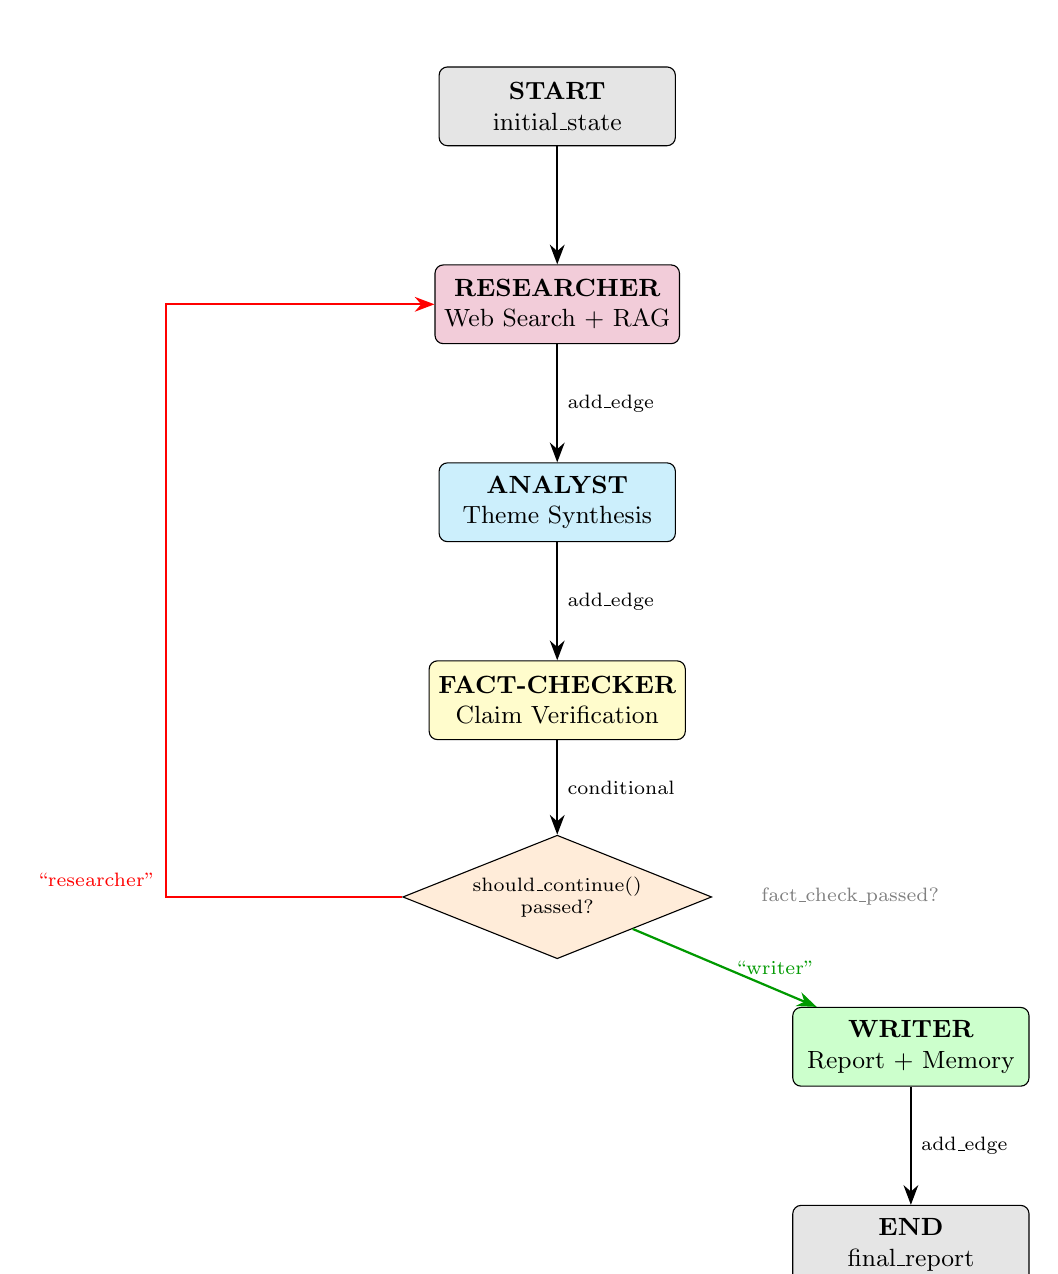
\begin{tikzpicture}[
    node distance=1.5cm,
    every node/.style={font=\small},
    box/.style={rectangle, draw, rounded corners=3pt, minimum width=3cm, minimum height=1cm, align=center},
    decision/.style={diamond, draw, aspect=2.5, minimum width=2cm, align=center, inner sep=2pt, font=\scriptsize},
    arrow/.style={-{Stealth[length=2.5mm]}, thick},
]

\node[box, fill=gray!20] (start) {\textbf{START}\\initial\_state};
\node[box, fill=purple!20, below=of start] (researcher) {\textbf{RESEARCHER}\\Web Search + RAG};
\node[box, fill=cyan!20, below=of researcher] (analyst) {\textbf{ANALYST}\\Theme Synthesis};
\node[box, fill=yellow!20, below=of analyst] (factchecker) {\textbf{FACT-CHECKER}\\Claim Verification};
\node[decision, fill=orange!15, below=1.2cm of factchecker] (decision) {should\_continue()\\passed?};
\node[box, fill=green!20, below right=1cm and 2cm of decision] (writer) {\textbf{WRITER}\\Report + Memory};
\node[box, fill=gray!20, below=of writer] (end) {\textbf{END}\\final\_report};

\draw[arrow] (start) -- (researcher);
\draw[arrow] (researcher) -- node[right, font=\scriptsize] {add\_edge} (analyst);
\draw[arrow] (analyst) -- node[right, font=\scriptsize] {add\_edge} (factchecker);
\draw[arrow] (factchecker) -- node[right, font=\scriptsize] {conditional} (decision);
\draw[arrow, green!60!black, thick] (decision) -- node[right, font=\scriptsize\color{green!60!black}] {``writer''} (writer);
\draw[arrow, red, thick] (decision.west) -| node[above left, font=\scriptsize\color{red}] {``researcher''} ++(-3,0) |- (researcher.west);
\draw[arrow] (writer) -- node[right, font=\scriptsize] {add\_edge} (end);

\node[right=0.5cm of decision, font=\scriptsize\color{gray}] {fact\_check\_passed?};
\end{tikzpicture}
\end{center}

\subsection{.invoke() vs .stream() --- Two Execution Modes}

\begin{conceptbox}{Graph Execution Modes}
Compiled graph ko 2 tarike se run kar sakte hain:

\textbf{1. invoke() --- Synchronous, Full Run:}
\begin{lstlisting}[style=pythonstyle]
result = research_graph.invoke(
    initial_state,            # Starting state
    {"recursion_limit": 25}   # Safety limit
)
# Returns: final complete state with all fields filled
# Used by: MCP server, benchmark evaluator
\end{lstlisting}

\textbf{2. stream() --- Streaming, Node-by-Node Events:}
\begin{lstlisting}[style=pythonstyle]
for event in research_graph.stream(
    initial_state,
    {"recursion_limit": 25}
):
    for node_name, node_output in event.items():
        print(f"Node {node_name} completed!")
        # Each event = one node's output
# Used by: SSE streaming endpoint
\end{lstlisting}

\textbf{Difference:}
\begin{itemize}
    \item \texttt{invoke()} = wait karo jab tak sab nodes complete ho jaayein, phir final state return karo
    \item \texttt{stream()} = har node complete hone pe event yield karo --- real-time progress tracking ke liye perfect
\end{itemize}
\end{conceptbox}


% ═══════════════════════════════════════════════════════════════════════
% CHAPTER 7: RAG VECTOR STORE DEEP DIVE
% ═══════════════════════════════════════════════════════════════════════

\chapter{RAG Vector Store --- Document Memory System (Deep Dive)}

\begin{storybox}{RAG kya hai? Library ki tarah socho...}
RAG = \textbf{Retrieval-Augmented Generation}. Imagine tumhare paas ek personal library hai. Jab tumhe kisi topic pe essay likhna hai:
\begin{enumerate}
    \item Library mein jao (Vector Store)
    \item Relevant books dhunddho (Similarity Search)
    \item Relevant pages bookmark karo (Top-K Retrieval)
    \item Un pages ke notes ke saath essay likho (Augmented Generation)
\end{enumerate}
Bina library ke: Sirf memory se likho $\rightarrow$ galat facts, incomplete information (hallucination)

Library ke saath: Verified sources ke saath likho $\rightarrow$ accurate, well-cited report (RAG)
\end{storybox}

\section{How Vector Search Actually Works}

\begin{conceptbox}{Vector Embeddings --- Text to Numbers}
\textbf{Challenge:} Computers text nahi samajhte. ``AI in healthcare'' aur ``machine learning for medicine'' dono ka same meaning hai, but text comparison mein ye alag strings hain.

\textbf{Solution --- Embeddings:} Har text ko ek high-dimensional vector (list of numbers) mein convert karo. Similar meanings wale texts ke vectors close hote hain in vector space.

\begin{lstlisting}[style=pythonstyle]
# Example (simplified - actual vectors are 384-dimensional)
embed("AI in healthcare")     -> [0.23, 0.87, 0.12, ...]
embed("machine learning for medicine") -> [0.25, 0.85, 0.14, ...]
# ^^ Very similar vectors! Close in 384-D space

embed("pizza recipe")         -> [0.91, 0.02, 0.78, ...]
# ^^ Very different vector! Far in 384-D space

# Cosine similarity:
cosine_sim(healthcare, medicine) = 0.95  # Very similar!
cosine_sim(healthcare, pizza)    = 0.12  # Not similar at all
\end{lstlisting}

\textbf{Mathematical formula:}
$$\text{cosine\_similarity}(\vec{a}, \vec{b}) = \frac{\vec{a} \cdot \vec{b}}{|\vec{a}| \times |\vec{b}|} = \frac{\sum_{i=1}^{n} a_i b_i}{\sqrt{\sum_{i=1}^{n} a_i^2} \times \sqrt{\sum_{i=1}^{n} b_i^2}}$$

Result 0 se 1 ke beech hota hai: 0 = completely unrelated, 1 = identical meaning.
\end{conceptbox}

\section{Embedding Model: all-MiniLM-L6-v2}

\begin{lstlisting}[style=pythonstyle,caption={vector\_store.py --- Embedding Model Setup}]
from langchain_huggingface import HuggingFaceEmbeddings
from config.setting import EMBEDDING_MODEL

_embeddings = None  # Module-level cache

def get_embeddings():
    """Singleton: Load embedding model once, reuse forever"""
    global _embeddings
    if _embeddings is None:
        _embeddings = HuggingFaceEmbeddings(
            model_name=EMBEDDING_MODEL,
            # "sentence-transformers/all-MiniLM-L6-v2"
            # - 22M parameters (tiny!)
            # - 384-dimensional output
            # - Trained on 1B+ sentence pairs
            # - Supports 256 token input max

            model_kwargs={"device": "cpu"},
            # CPU pe chalta hai - no GPU needed
            # GPU available ho toh "cuda" set karo for 10x speed

            encode_kwargs={"normalize_embeddings": True},
            # L2 normalization: vectors ko unit length pe normalize
            # Benefit: cosine similarity = simple dot product
            # (faster computation)
        )
    return _embeddings
\end{lstlisting}

\begin{interviewbox}{Why did you choose all-MiniLM-L6-v2 for embeddings?}
\textbf{Answer:} ``Kaafi reasons hain: (1) \textbf{Size} --- sirf 22M parameters, model ~80MB hai, fast load hota hai CPU pe bhi. (2) \textbf{Quality} --- MTEB benchmark pe top-tier performance for its size class. (3) \textbf{Dimensions} --- 384-dimensional vectors, compact but effective --- ChromaDB mein kam storage lagta hai. (4) \textbf{Offline} --- HuggingFace se first time download hota hai, phir locally cached rehta hai --- no API calls, no cost. (5) \textbf{Compatibility} --- LangChain integration seamless hai via HuggingFaceEmbeddings wrapper. Production mein agar accuracy priority ho toh OpenAI text-embedding-3-small (1536 dimensions) pe upgrade kar sakte hain but woh paid hai.''
\end{interviewbox}

\section{Document Chunking Strategy}

\begin{lstlisting}[style=pythonstyle,caption={vector\_store.py --- Text Splitting}]
from langchain.text_splitter import RecursiveCharacterTextSplitter

def get_splitter():
    return RecursiveCharacterTextSplitter(
        chunk_size=CHUNK_SIZE,           # 1000 characters
        chunk_overlap=CHUNK_OVERLAP,     # 200 characters
        separators=["\n\n", "\n", ". ", " ", ""],
        # Hierarchy: paragraph > line > sentence > word > char
    )
\end{lstlisting}

\begin{conceptbox}{Chunking Parameters --- Trade-offs Explained}
\begin{center}
\begin{tabular}{|p{3cm}|p{5cm}|p{5cm}|}
\hline
\textbf{Parameter} & \textbf{Too Small} & \textbf{Too Large} \\
\hline
chunk\_size & Context meaning toot jaata hai & Irrelevant content include hota hai \\
\hline
chunk\_overlap & Context boundary pe info loss & Redundant storage, slower search \\
\hline
\end{tabular}
\end{center}

\textbf{1000/200 kyun?}
\begin{itemize}
    \item 1000 chars $\approx$ 250 words $\approx$ 1 paragraph --- ek coherent thought unit
    \item 200 chars overlap $\approx$ 50 words --- agar sentence chunk boundary pe toote toh next chunk mein bhi available ho
\end{itemize}

\textbf{Separator hierarchy:}
\begin{lstlisting}[language={}]
"\n\n"  -> Paragraph break (best split point)
"\n"    -> Line break (good split point)
". "    -> Sentence end (decent split point)
" "     -> Word boundary (last resort)
""      -> Character level (emergency only)
\end{lstlisting}
RecursiveCharacterTextSplitter pehle best separator try karta hai. Agar chunk\_size exceed ho toh next separator pe fall through karta hai.
\end{conceptbox}

\section{All RAG Operations}

\subsection{PDF Ingestion Pipeline}

\begin{lstlisting}[style=pythonstyle]
def ingest_documents(file_paths):
    """Ingest PDFs into research_docs collection"""
    vectorstore = get_vectorstore("research_docs")
    splitter = get_splitter()
    total_chunks = 0

    for path in file_paths:
        # Step 1: Parse PDF pages
        loader = PyPDFLoader(path)
        docs = loader.load()
        # Each doc = one PDF page with page_content + metadata

        # Step 2: Split pages into chunks
        chunks = splitter.split_documents(docs)
        # A 10-page PDF might produce ~30-50 chunks

        # Step 3: Embed + Store in ChromaDB
        if chunks:
            vectorstore.add_documents(documents=chunks)
            # Internally:
            # 1. Get embedding for each chunk's text
            # 2. Store embedding vector + original text in ChromaDB
            total_chunks += len(chunks)

    return {
        "chunks_added": total_chunks,
        "files_processed": [os.path.basename(p) for p in file_paths]
    }
\end{lstlisting}

\subsection{Similarity Search}

\begin{lstlisting}[style=pythonstyle]
def retrieve_context(query, collection_name="research_docs", k=5):
    """Find top-k most relevant chunks for a query"""
    vs = get_vectorstore(collection_name)
    results = vs.similarity_search(query, k=k)
    # Internally:
    # 1. Embed the query text -> 384-dim vector
    # 2. Find k nearest vectors in ChromaDB (cosine distance)
    # 3. Return corresponding text chunks

    return [doc.page_content for doc in results]
\end{lstlisting}

\subsection{Research Memory Storage}

\begin{lstlisting}[style=pythonstyle]
def store_research_session(topic, research_data, report):
    """Save completed research to past_research collection"""
    # Combine topic + report + sources into one document
    combined = f"TOPIC: {topic}\n\nREPORT:\n{report}\n\n"
    combined += "SOURCES:\n" + "\n---\n".join(research_data[:5])

    # Create LangChain Document object
    docs = [Document(
        page_content=combined,
        metadata={"topic": topic, "type": "research_session"}
    )]

    # Chunk the combined document
    chunks = get_splitter().split_documents(docs)

    # Store in past_research collection
    vs = get_vectorstore("past_research")
    vs.add_documents(documents=chunks)

    return len(chunks)  # Number of chunks stored
\end{lstlisting}


% ═══════════════════════════════════════════════════════════════════════
% CHAPTER 8: DJANGO REST FRAMEWORK BACKEND (COMPREHENSIVE)
% ═══════════════════════════════════════════════════════════════════════

\chapter{Django REST Framework Backend --- Complete API Layer}

\section{Django Settings --- Production Configuration}

\begin{lstlisting}[style=pythonstyle,caption={backend/orchestrator\_backend/settings.py}]
# Application definition
INSTALLED_APPS = [
    'django.contrib.admin',       # Admin panel
    'django.contrib.auth',        # User authentication
    'django.contrib.contenttypes',# Content type framework
    'django.contrib.sessions',    # Session management
    'django.contrib.messages',    # Flash messages
    'django.contrib.staticfiles', # Static file serving
    'rest_framework',             # DRF core
    'rest_framework.authtoken',   # Token authentication
    'corsheaders',                # CORS support
    'api',                        # Our research API app
]

# DRF Configuration
REST_FRAMEWORK = {
    'DEFAULT_AUTHENTICATION_CLASSES': [
        'rest_framework.authentication.TokenAuthentication',
        # ^^ Primary: Token-based auth via Authorization header
        'rest_framework.authentication.SessionAuthentication',
        # ^^ Secondary: Cookie-based auth for browsable API
    ],
    'DEFAULT_PERMISSION_CLASSES': [
        'rest_framework.permissions.IsAuthenticated',
        # ^^ Default: all endpoints require authentication
        # Individual views override with AllowAny where needed
    ],
    'DEFAULT_THROTTLE_CLASSES': [
        'rest_framework.throttling.AnonRateThrottle',
        'rest_framework.throttling.UserRateThrottle',
    ],
    'DEFAULT_THROTTLE_RATES': {
        'anon': '30/minute',     # Anonymous: 30 req/min
        'user': '120/minute',    # Authenticated: 120 req/min
    },
    # ^^ Rate limiting prevents abuse
}
\end{lstlisting}

\section{Database Models --- Complete Schema}

\subsection{ResearchSession --- Main Entity}

\begin{lstlisting}[style=pythonstyle]
class ResearchSession(models.Model):
    STATUS_CHOICES = [
        ("queued", "Queued"),       # Job created, not started
        ("running", "Running"),     # Pipeline executing
        ("completed", "Completed"), # Successfully finished
        ("failed", "Failed"),       # Error occurred
    ]

    # === OWNERSHIP ===
    user = models.ForeignKey(
        User, on_delete=models.CASCADE,
        null=True, blank=True
        # null=True allows anonymous research
        # CASCADE: delete user -> delete their sessions
    )

    # === CORE DATA ===
    topic = models.CharField(max_length=512)
    status = models.CharField(
        max_length=20,
        choices=STATUS_CHOICES,
        default="completed"
    )
    final_report = models.TextField()

    # === DENORMALIZED COUNTERS ===
    web_sources_count = models.IntegerField(default=0)
    rag_chunks_count = models.IntegerField(default=0)
    revision_count = models.IntegerField(default=0)
    # ^^ Why denormalized? Performance!
    # Instead of: session.sources.filter(type='web').count()
    # We do: session.web_sources_count (instant, no query)

    # === TIMING ===
    duration_seconds = models.FloatField(null=True, blank=True)
    started_at = models.DateTimeField(null=True, blank=True)
    completed_at = models.DateTimeField(null=True, blank=True)
    created_at = models.DateTimeField(auto_now_add=True)

    # === QUALITY DATA ===
    fact_check_result = models.TextField(blank=True)

    # === ERROR TRACKING ===
    error_code = models.CharField(max_length=64, blank=True)
    error_message = models.TextField(blank=True)

    # === SSE SUPPORT ===
    progress_version = models.PositiveIntegerField(default=0)
    # Incremented on each event -> client knows if new events exist

    class Meta:
        ordering = ["-created_at"]  # Newest first
        indexes = [
            models.Index(fields=["user", "-created_at"]),
            # Composite index: fast "get user's recent sessions"
        ]
\end{lstlisting}

\subsection{ResearchEvent --- Timeline Events}

\begin{lstlisting}[style=pythonstyle]
class ResearchEvent(models.Model):
    STAGE_CHOICES = [
        ("queued", "Queued"),
        ("researcher", "Researcher"),
        ("analyst", "Analyst"),
        ("fact_checker", "Fact-Checker"),
        ("writer", "Writer"),
        ("completed", "Completed"),
        ("failed", "Failed"),
    ]

    session = models.ForeignKey(
        ResearchSession,
        related_name="events",  # session.events.all()
        on_delete=models.CASCADE
    )
    sequence = models.PositiveIntegerField()
    # ^^ Order number: 0, 1, 2, 3...
    stage = models.CharField(max_length=32, choices=STAGE_CHOICES)
    message = models.CharField(max_length=1000)
    created_at = models.DateTimeField(auto_now_add=True)

    class Meta:
        ordering = ["sequence"]
        constraints = [
            models.UniqueConstraint(
                fields=["session", "sequence"],
                name="research_event_session_sequence"
            )
            # ^^ Same session can't have 2 events
            #    with same sequence number
        ]
\end{lstlisting}

\subsection{ResearchSource --- Evidence Preservation}

\begin{lstlisting}[style=pythonstyle]
class ResearchSource(models.Model):
    SOURCE_TYPE_CHOICES = [
        ("web", "Web"),   # From Tavily/DuckDuckGo search
        ("rag", "RAG"),   # From ChromaDB retrieval
    ]

    session = models.ForeignKey(
        ResearchSession,
        related_name="sources",
        on_delete=models.CASCADE
    )
    source_type = models.CharField(max_length=16,
                                  choices=SOURCE_TYPE_CHOICES)
    position = models.PositiveIntegerField()
    url = models.URLField(blank=True, max_length=2048)
    title = models.CharField(max_length=512, blank=True)
    domain = models.CharField(max_length=255, blank=True)
    # ^^ Parsed from URL for display (e.g., "arxiv.org")
    snippet = models.TextField()
    # ^^ First ~500 chars of source content
\end{lstlisting}

\section{Token Authentication System}

\begin{lstlisting}[style=pythonstyle,caption={views.py --- Registration + Login}]
class RegisterAPIView(APIView):
    permission_classes = [permissions.AllowAny]
    # ^^ Registration doesn't need auth (obviously!)

    def post(self, request):
        serializer = RegisterSerializer(data=request.data)
        if serializer.is_valid():
            user = serializer.save()

            # Create auth token for immediate login
            token, _ = Token.objects.get_or_create(user=user)

            return Response({
                "user": UserSerializer(user).data,
                "token": token.key,
                # ^^ Client stores this token in localStorage
                "message": "User registered successfully",
            }, status=status.HTTP_201_CREATED)

        return Response(serializer.errors, status=400)


class LoginAPIView(APIView):
    permission_classes = [permissions.AllowAny]

    def post(self, request):
        user = authenticate(
            username=request.data.get("username"),
            password=request.data.get("password")
        )
        if user:
            token, _ = Token.objects.get_or_create(user=user)
            return Response({
                "user": UserSerializer(user).data,
                "token": token.key,
            })
        return Response(
            {"error": "Invalid credentials"},
            status=status.HTTP_401_UNAUTHORIZED
        )
\end{lstlisting}

\begin{conceptbox}{Token Authentication Complete Flow}
\begin{center}
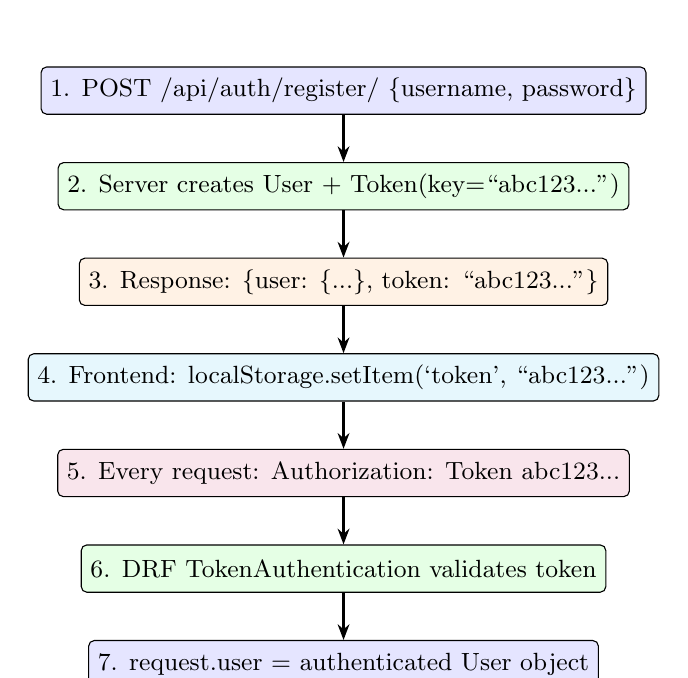
\begin{tikzpicture}[
    node distance=0.6cm,
    box/.style={rectangle, draw, rounded corners=2pt, minimum width=5cm, minimum height=0.6cm, align=center, font=\small},
    arrow/.style={-{Stealth[length=2mm]}, thick},
]
\node[box, fill=blue!10] (reg) {1. POST /api/auth/register/ \{username, password\}};
\node[box, fill=green!10, below=of reg] (token) {2. Server creates User + Token(key=``abc123...'')};
\node[box, fill=orange!10, below=of token] (resp) {3. Response: \{user: \{...\}, token: ``abc123...''\}};
\node[box, fill=cyan!10, below=of resp] (store) {4. Frontend: localStorage.setItem(`token', ``abc123...'')};
\node[box, fill=purple!10, below=of store] (req) {5. Every request: Authorization: Token abc123...};
\node[box, fill=green!10, below=of req] (auth) {6. DRF TokenAuthentication validates token};
\node[box, fill=blue!10, below=of auth] (user) {7. request.user = authenticated User object};
\draw[arrow] (reg) -- (token);
\draw[arrow] (token) -- (resp);
\draw[arrow] (resp) -- (store);
\draw[arrow] (store) -- (req);
\draw[arrow] (req) -- (auth);
\draw[arrow] (auth) -- (user);
\end{tikzpicture}
\end{center}
\end{conceptbox}

\section{Durable Job Execution System}

\begin{lstlisting}[style=pythonstyle,caption={services.py --- Background Job Runner}]
import threading
from django.db import close_old_connections

def queue_research_job(user, topic):
    """Create a new research session in 'queued' state"""
    session = ResearchSession.objects.create(
        user=user,
        topic=topic,
        status="queued",
        final_report="",
    )
    _record_event(session, "queued",
                  f"Research job queued: {topic}")
    return session


def launch_research_job(session_id, asynchronous=True):
    """Launch the research pipeline"""
    if asynchronous:
        thread = threading.Thread(
            target=run_research_job,
            args=(session_id,),
            daemon=True,
            # daemon=True: thread dies when main process exits
            # Important: prevents zombie threads
        )
        thread.start()
    else:
        # Synchronous mode for testing
        run_research_job(session_id)


def run_research_job(session_id):
    """Execute the full research pipeline"""
    close_old_connections()
    # ^^ Critical for threaded Django code!
    # Thread might have inherited stale DB connection from parent

    session = ResearchSession.objects.get(pk=session_id)
    session.status = "running"
    session.started_at = timezone.now()
    session.save()
    _record_event(session, "researcher", "Pipeline starting...")

    try:
        # Import here to avoid circular imports
        from graph.workflow import research_graph
        from config.providers import initial_research_state

        initial_state = initial_research_state(session.topic)

        # === EXECUTE LANGGRAPH PIPELINE ===
        result = research_graph.invoke(
            initial_state,
            {"recursion_limit": 25}
        )

        # === PERSIST RESULTS ===
        session.final_report = result.get("final_report", "")
        session.fact_check_result = result.get("fact_check_result", "")
        session.revision_count = result.get("revision_count", 0)
        session.status = "completed"
        session.completed_at = timezone.now()
        session.duration_seconds = round(
            (session.completed_at - session.started_at).total_seconds(),
            2
        )
        session.save()

        # Store sources
        _store_sources(session, result.get("research_data", []),
                       result.get("rag_context", []))

        _record_event(session, "completed",
                      f"Research complete in {session.duration_seconds}s")

    except Exception as exc:
        # === ERROR HANDLING ===
        session.status = "failed"
        session.error_code = "research_execution_failed"
        session.error_message = str(exc)[:1000]
        session.completed_at = timezone.now()
        session.save()
        _record_event(session, "failed", f"Error: {str(exc)[:200]}")

    finally:
        close_old_connections()
        # ^^ Always cleanup DB connections in thread
\end{lstlisting}

\section{SSE Streaming Implementation}

\begin{lstlisting}[style=pythonstyle,caption={views.py --- Server-Sent Events Streaming}]
class ResearchStreamAPIView(APIView):
    permission_classes = [permissions.IsAuthenticated]

    def post(self, request):
        topic = request.data.get("topic", "")
        if not topic:
            return Response({"error": "Topic required"}, status=400)

        session = queue_research_job(request.user, topic)

        def event_stream():
            """Generator that yields SSE events"""
            from graph.workflow import research_graph
            from config.providers import initial_research_state

            state = initial_research_state(topic)
            completed_session_id = session.id

            # Stream graph execution node-by-node
            for event in research_graph.stream(
                state, {"recursion_limit": 25}
            ):
                for node_name, node_output in event.items():
                    if node_name == "__end__":
                        continue

                    # Extract latest message from agent
                    messages = node_output.get("messages", [])
                    msg = messages[-1] if messages else f"{node_name} done"

                    # Yield SSE-formatted event
                    yield f"data: {json.dumps({
                        'stage': node_name,
                        'message': msg,
                        'session_id': completed_session_id,
                    })}\n\n"
                    # ^^ SSE format: "data: {json}\n\n"
                    # Double newline separates events

                    # Persist event to DB
                    _record_event(session, node_name, msg)

                    # Update state for final persistence
                    state.update(node_output)

            # Save final results
            session.final_report = state.get("final_report", "")
            session.status = "completed"
            session.save()

            # Signal stream end
            yield "data: [DONE]\n\n"

        return StreamingHttpResponse(
            event_stream(),
            content_type="text/event-stream",
            headers={
                "Cache-Control": "no-cache",
                # ^^ Don't cache streaming responses

                "X-Accel-Buffering": "no",
                # ^^ Nginx: don't buffer, send immediately

                "Connection": "keep-alive",
                # ^^ Keep TCP connection open for streaming
            }
        )
\end{lstlisting}

\section{Export System --- 4 Formats}

\begin{lstlisting}[style=pythonstyle,caption={views.py --- Multi-Format Export}]
class ExportReportAPIView(APIView):
    permission_classes = [permissions.AllowAny]
    # ^^ Allow unauthenticated export for sharing

    def get(self, request, pk):
        session = get_object_or_404(ResearchSession, pk=pk)
        fmt = request.query_params.get("format", "markdown")
        report = session.final_report or "No report available."

        if fmt == "json":
            # Full structured JSON export
            data = ResearchSessionDetailSerializer(session).data
            return Response(data)

        elif fmt == "bibtex":
            # Academic citation format
            bib_entries = []
            for i, src in enumerate(session.sources.all(), 1):
                entry = (
                    f"@misc{{maro_{session.id}_{i},\n"
                    f"  title = {{{src.title or 'Untitled'}}},\n"
                    f"  url = {{{src.url}}},\n"
                    f"  note = {{Retrieved by MARO}}\n"
                    f"}}"
                )
                bib_entries.append(entry)
            bib_content = "\n\n".join(bib_entries)
            return HttpResponse(bib_content,
                               content_type="text/plain")

        elif fmt == "html":
            # Styled HTML page
            html = f"""<!DOCTYPE html>
            <html><head>
              <title>{session.topic} - MARO Report</title>
              <style>
                body {{ font-family: Georgia, serif;
                       max-width: 800px; margin: 0 auto;
                       padding: 2rem; color: #333; }}
                h1 {{ color: #1a1a2e; }}
                a {{ color: #6366f1; }}
              </style>
            </head><body>
              <h1>{session.topic}</h1>
              <p><em>Generated by MARO | {session.created_at}</em></p>
              <hr>
              {markdown.markdown(report)}
            </body></html>"""
            return HttpResponse(html, content_type="text/html")

        else:  # markdown (default)
            return HttpResponse(
                report,
                content_type="text/markdown",
                headers={"Content-Disposition":
                    f'attachment; filename="{session.topic[:30]}.md"'}
            )
\end{lstlisting}

\section{Complete API Endpoints Reference}

\begin{longtable}{|p{1cm}|p{4.5cm}|p{1.5cm}|p{6cm}|}
\hline
\textbf{Verb} & \textbf{Endpoint} & \textbf{Auth?} & \textbf{Description} \\
\hline
\endhead
GET & /api/health/ & No & Server health check + active provider \\
\hline
POST & /api/auth/register/ & No & Create new user, return token \\
\hline
POST & /api/auth/login/ & No & Authenticate user, return token \\
\hline
POST & /api/auth/logout/ & Yes & Delete auth token (server-side) \\
\hline
GET & /api/auth/profile/ & Yes & Get current user profile \\
\hline
PUT & /api/auth/profile/ & Yes & Update username/email \\
\hline
POST & /api/auth/change-password/ & Yes & Change password, re-issue token \\
\hline
POST & /api/research/execute/ & No & Synchronous research (legacy) \\
\hline
GET & /api/research/jobs/ & Yes & List user's research jobs \\
\hline
POST & /api/research/jobs/ & Yes & Create new research job (async) \\
\hline
POST & /api/research/stream/ & Yes & SSE streaming research pipeline \\
\hline
POST & /api/research/documents/ & Yes & Upload PDFs to ChromaDB \\
\hline
GET & /api/research/sessions/ & Yes & List sessions (paginated) \\
\hline
GET & /api/research/sessions/\{id\}/ & Yes & Get session detail (full report) \\
\hline
DEL & /api/research/sessions/\{id\}/ & Yes & Delete session (owner only) \\
\hline
GET & /api/research/sessions/\{id\}/export/ & No & Export (md/html/json/bibtex) \\
\hline
GET & /api/research/\{id\}/tags/ & Yes & List session tags \\
\hline
POST & /api/research/\{id\}/tags/ & Yes & Add tag to session \\
\hline
POST & /api/research/benchmark/ & No & Run benchmark comparison \\
\hline
GET & /api/benchmark/history/ & No & List past benchmarks \\
\hline
GET & /api/stats/ & No & Platform analytics dashboard \\
\hline
GET & /api/rag/stats/ & No & ChromaDB collection stats \\
\hline
POST & /api/rag/search/ & No & Direct RAG query \\
\hline
\end{longtable}


% ═══════════════════════════════════════════════════════════════════════
% CHAPTER 9: REACT FRONTEND
% ═══════════════════════════════════════════════════════════════════════

\chapter{React + Vite Frontend --- Complete UI System}

\section{API Client Class --- api.js}

\begin{lstlisting}[style=jsstyle,caption={api.js --- Complete Client Architecture}]
const API_BASE = (import.meta.env.VITE_API_URL || '') + '/api';
// import.meta.env.VITE_API_URL -> Vite env variable
// Default: '' (same origin - Django serves frontend too)
// Dev: 'http://localhost:8000' (separate Django server)

class ApiClient {
  constructor() {
    // Restore token from localStorage (persistent login)
    this.token = localStorage.getItem('maro_auth_token') || '';
  }

  setToken(token) {
    this.token = token || '';
    if (token) {
      localStorage.setItem('maro_auth_token', token);
    } else {
      localStorage.removeItem('maro_auth_token');
    }
  }

  getHeaders(isMultipart = false) {
    const headers = {};
    if (!isMultipart) {
      headers['Content-Type'] = 'application/json';
    }
    // ^^ Don't set Content-Type for FormData (file uploads)
    // Browser sets it automatically with boundary

    if (this.token) {
      headers['Authorization'] = `Token ${this.token}`;
    }
    return headers;
  }

  async request(endpoint, options = {}) {
    const url = `${API_BASE}${endpoint}`;
    const res = await fetch(url, {
      ...options,
      headers: {
        ...this.getHeaders(options.isMultipart),
        ...(options.headers || {})
      },
    });

    if (res.status === 204) return null;
    // 204 No Content -> no body to parse

    const data = await res.json().catch(() => ({}));

    if (!res.ok) {
      throw new Error(data.error || data.detail || 'Request failed');
    }
    return data;
  }

  // === AUTH METHODS ===
  async login(username, password) {
    const data = await this.request('/auth/login/', {
      method: 'POST',
      body: JSON.stringify({ username, password }),
    });
    this.setToken(data.token);
    return data;
  }

  async register(username, email, password) {
    const data = await this.request('/auth/register/', {
      method: 'POST',
      body: JSON.stringify({ username, email, password }),
    });
    this.setToken(data.token);
    return data;
  }

  logout() {
    this.request('/auth/logout/', { method: 'POST' }).catch(() => {});
    this.setToken('');
  }

  // === SSE STREAMING ===
  async streamResearch(topic, { onEvent, onError, onComplete }) {
    const response = await fetch(`${API_BASE}/research/stream/`, {
      method: 'POST',
      headers: this.getHeaders(),
      body: JSON.stringify({ topic }),
    });

    if (!response.ok) {
      const err = await response.json().catch(() => ({}));
      throw new Error(err.error || 'Stream failed');
    }

    // Read SSE stream chunk by chunk
    const reader = response.body.getReader();
    const decoder = new TextDecoder('utf-8');
    let buffer = '';
    let completedSessionId = null;

    while (true) {
      const { value, done } = await reader.read();
      if (done) break;

      buffer += decoder.decode(value, { stream: true });
      // { stream: true } -> don't flush incomplete characters

      const lines = buffer.split('\n');
      buffer = lines.pop();
      // ^^ Keep last (possibly incomplete) line in buffer

      for (const line of lines) {
        const trimmed = line.trim();
        if (!trimmed.startsWith('data:')) continue;

        const dataStr = trimmed.slice(5).trim();
        // Remove "data: " prefix

        if (dataStr === '[DONE]') {
          onComplete({ sessionId: completedSessionId });
          return;
        }

        try {
          const eventData = JSON.parse(dataStr);
          completedSessionId = eventData.session_id;
          onEvent(eventData);
          // eventData = { stage, message, session_id }
        } catch (e) {
          console.warn('Failed to parse SSE event:', dataStr);
        }
      }
    }
  }
}

export const api = new ApiClient();
// ^^ Singleton export - entire app uses same instance
\end{lstlisting}

\section{ResearchStudio --- Core Component Analysis}

\begin{conceptbox}{ResearchStudio Features (861 lines)}
Ye sabse bada aur most important component hai:

\begin{enumerate}
    \item \textbf{Topic Input Panel:} Textarea + suggestion chips (pre-defined topics)
    \item \textbf{RAG File Upload:} Drag-and-drop PDF upload with progress indicator
    \item \textbf{Pipeline Parameters:} Sliders for Max Revisions, Top-K chunks, Verification Rigor
    \item \textbf{Launch Button:} Animated button with loading state
    \item \textbf{Live Streaming Terminal:} Real-time SSE events with timestamps, colored by agent
    \item \textbf{Agent Graph Visualizer:} 4-step pipeline status tracker (active/done/pending)
    \item \textbf{Results Panel with 3 Tabs:}
    \begin{itemize}
        \item Report Tab: Markdown rendered via marked.js
        \item Evidence Tab: Source cards with URLs, domains, snippets
        \item Fact-Check Tab: Verification analysis with score badges
    \end{itemize}
    \item \textbf{Export Actions:} Copy to clipboard, Download MD, Download HTML, Download BibTeX
    \item \textbf{Tags System:} Add/view tags on completed sessions
    \item \textbf{Confetti:} canvas-confetti animation on successful completion
\end{enumerate}
\end{conceptbox}

\section{AgentGraph --- Pipeline Visualizer Component}

\begin{lstlisting}[style=jsstyle,caption={AgentGraph.jsx --- Complete Code}]
export default function AgentGraph({ currentStage, revisionCount,
                                     isRunning }) {
  const steps = [
    { id: 'researcher', num: '01', label: 'RESEARCHER',
      role: 'Dual-Vector & Web Search', icon: Search },
    { id: 'analyst', num: '02', label: 'ANALYST',
      role: 'Contradiction & Theme Synthesis', icon: Brain },
    { id: 'fact_checker', num: '03', label: 'FACT-CHECKER',
      role: 'Claim Verification Gate', icon: ShieldCheck },
    { id: 'writer', num: '04', label: 'WRITER',
      role: 'Synthesis & Memory Storage', icon: PenTool }
  ];

  const getStageIndex = (stage) => {
    switch (stage) {
      case 'researcher': return 0;
      case 'analyst': return 1;
      case 'fact_checker': return 2;
      case 'writer': return 3;
      case 'completed': return 4;
      default: return -1;
    }
  };

  const activeIdx = getStageIndex(currentStage);

  return (
    <div style={{ display: 'grid',
                  gridTemplateColumns: 'repeat(auto-fit, minmax(220px, 1fr))',
                  gap: '0.75rem' }}>
      {steps.map((step, idx) => {
        const isActive = currentStage === step.id && isRunning;
        const isDone = currentStage === 'completed' || activeIdx > idx;
        // Active = currently processing (cyan glow)
        // Done = already completed (green check)
        // Pending = not yet reached (dim gray)

        return (
          <div key={step.id} style={{
            border: isActive ? '1px solid cyan'
                  : isDone ? '1px solid green'
                  : '1px solid gray',
            boxShadow: isActive ? '0 0 16px rgba(0,245,243,0.25)'
                     : 'none',
            // ^^ Active agent gets a glowing border effect
          }}>
            {isDone ? <Check /> : step.num}
            <div>{step.label}</div>
            <div>{step.role}</div>
          </div>
        );
      })}
    </div>
  );
}
\end{lstlisting}


% ═══════════════════════════════════════════════════════════════════════
% CHAPTER 10: MCP SERVER
% ═══════════════════════════════════════════════════════════════════════

\chapter{FastMCP Server --- AI Tool Integration}

\begin{storybox}{MCP ka concept}
MCP = Model Context Protocol. Imagine tum Claude Desktop mein baithe ho aur bolte ho ``Mujhe quantum computing pe research chahiye.'' Normally Claude apne training data se answer dega. But MCP ke through, Claude directly humara MARO pipeline invoke kar sakta hai --- real-time web search + 4-agent analysis + fact-checking + final report --- sab Claude ke andar se!

\textbf{Matlab:} Humara research system ek ``plugin'' ban jaata hai jo koi bhi AI assistant use kar sakta hai.
\end{storybox}

\begin{lstlisting}[style=pythonstyle,caption={mcp\_server.py --- Server Setup}]
from fastmcp import FastMCP, Context
from pydantic import BaseModel, Field, field_validator

mcp = FastMCP(
    "research_orchestrator_mcp",
    instructions=(
        "Multi-Agent Research Orchestrator -- 4 AI agents "
        "collaborate to research, analyze, fact-check, and "
        "write reports on any topic. Supports Groq, OpenAI, "
        "Anthropic, and Ollama providers."
    ),
    # ^^ instructions tells the AI assistant what this server does
)

# === PYDANTIC INPUT VALIDATION ===
class ResearchTopicInput(BaseModel):
    topic: str = Field(
        ...,              # ... = required
        description="Research topic (3-500 chars)",
        min_length=3,
        max_length=500,
    )
    # Pydantic validates before our code even runs!
    # Invalid input -> clean error message to AI assistant

class SearchKnowledgeInput(BaseModel):
    query: str = Field(..., min_length=2, max_length=300)
    num_results: int = Field(default=5, ge=1, le=20)
    # ge=1: greater than or equal to 1
    # le=20: less than or equal to 20

# === MCP TOOL REGISTRATION ===
@mcp.tool(
    name="research_orchestrator_research_topic",
    annotations={
        "readOnlyHint": False,   # Modifies state (creates session)
        "destructiveHint": False, # Doesn't delete anything
        "idempotentHint": False,  # Different results each time
        "openWorldHint": True,   # Calls external APIs
    },
)
async def research_topic(params: ResearchTopicInput,
                         ctx: Context) -> str:
    """Run the full 4-agent research pipeline."""
    await ctx.report_progress(0.0, f"Starting: {params.topic}")
    # ^^ Progress reporting -> AI assistant shows loading bar

    from graph.workflow import research_graph

    initial_state = {
        "topic": params.topic,
        "research_data": [], "analysis": "",
        "fact_check_result": "", "fact_check_passed": False,
        "revision_count": 0, "final_report": "",
        "rag_context": [], "messages": [],
        "current_agent": "", "error": "",
    }
    # ^^ MCP server builds its own initial_state
    # Independent of Django models

    result = research_graph.invoke(initial_state,
                                  {"recursion_limit": 25})
    report = result.get("final_report", "No report generated.")

    await ctx.report_progress(1.0, "Research complete")
    return f"# Research Report: {params.topic}\n\n{report}"
    # Return value goes directly to AI assistant

# === ENTRY POINT ===
if __name__ == "__main__":
    mcp.run(transport="stdio")
    # stdio transport: communicates via stdin/stdout
    # AI assistant spawns this process and talks via pipes
\end{lstlisting}


% ═══════════════════════════════════════════════════════════════════════
% CHAPTER 11: BENCHMARK SYSTEM
% ═══════════════════════════════════════════════════════════════════════

\chapter{Benchmark Arena --- Empirical Evaluation System}

\section{Why Benchmarking?}

\begin{storybox}{``Prove karo ki better hai!''}
Interviewer zaroor poochega: ``Tum claim karte ho multi-agent better hai --- data hai kya?''

Isliye humne Benchmark Arena banaya. Ye ek hi topic pe 2 approaches chalata hai:
\begin{enumerate}
    \item \textbf{Single-Agent:} Ek LLM call, no search, no verification
    \item \textbf{Multi-Agent:} Full 4-agent pipeline with search + revision
\end{enumerate}
Phir dono ko Depth Score aur Verifiability Score pe rate karta hai.
\end{storybox}

\section{Dual Scoring System}

\begin{lstlisting}[style=pythonstyle,caption={evaluator.py --- Heuristic Scoring Functions}]
def _depth_score(text):
    """Structural depth heuristic (0-10)"""
    if not text: return 0
    headings = len(re.findall(r"^#{1,4}\s.+$", text, re.MULTILINE))
    # Count Markdown headings (# to ####)

    bullets = len(re.findall(r"^\s*[-*+]\s", text, re.MULTILINE))
    # Count bullet points

    words = len(text.split())
    # Total word count

    score = min(headings, 8) + min(bullets//4, 4) + min(words//150, 3)
    # Max 8 points from headings
    # Max 4 points from bullets (1 point per 4 bullets)
    # Max 3 points from length (1 point per 150 words)
    # Total max: 8 + 4 + 3 = 15, clamped to 10

    return max(0, min(10, score))


def _verifiability_score(text):
    """Citation quality heuristic (0-10)"""
    if not text: return 0
    urls = len(re.findall(r"https?://\S+", text))
    # Count HTTP/HTTPS URLs

    citations = len(re.findall(
        r"\[\d+\]|\[Source[:\]]|\(Source[:\s]",
        text, re.IGNORECASE
    ))
    # Count inline citations like [1], [Source], (Source:...)

    score = min(urls, 5) * 1.5 + min(citations, 5)
    # Max 7.5 from URLs + Max 5 from citations = 12.5
    return max(0, min(10, int(score)))
\end{lstlisting}

\begin{conceptbox}{LLM-as-Judge Pattern}
Heuristic scores basic hain (regex-based). LLM-as-Judge zyada nuanced scoring deta hai:

\begin{lstlisting}[style=pythonstyle]
JUDGE_PROMPT = """Score BOTH reports from 0 to 10 on:
- depth_score: structure, coverage, multiple angles
- verifiability_score: grounded claims, citations

Return ONLY valid JSON:
{"single_agent": {"depth_score": N, "verifiability_score": N},
 "multi_agent": {"depth_score": N, "verifiability_score": N},
 "verdict": "MULTI_AGENT_SUPERIOR"}
"""

llm = get_llm_with_fallback(model=None, temperature=0.0)
# temperature=0.0: Judge must be DETERMINISTIC
# Same inputs should give same scores
\end{lstlisting}

\textbf{Dual approach:} Heuristics always work (no LLM needed). LLM judge augments when available. If LLM fails, heuristics are the fallback. Ye \textbf{``belt and suspenders''} approach hai.
\end{conceptbox}


% ═══════════════════════════════════════════════════════════════════════
% CHAPTER 12: TESTING STRATEGY
% ═══════════════════════════════════════════════════════════════════════

\chapter{Testing Strategy --- 62 Tests, 100\% Pass}

\begin{conceptbox}{Test Architecture}
\begin{lstlisting}[language={}]
backend/api/tests/
|-- conftest.py           # Shared fixtures
|-- test_auth.py          # 14 tests - Authentication
|-- test_benchmark.py     # 10 tests - Benchmarking
|-- test_research.py      # 14 tests - Research pipeline
|-- test_research_jobs.py #  6 tests - Job management
|-- test_platform_features.py # 10 tests - Stats, RAG, Tags
|-- test_streaming.py     #  4 tests - SSE streaming
|-- test_tags.py          #  4 tests - Tag CRUD
\end{lstlisting}
\end{conceptbox}

\begin{lstlisting}[style=pythonstyle,caption={conftest.py --- Test Fixtures}]
import pytest
from rest_framework.test import APIClient
from django.contrib.auth.models import User
from rest_framework.authtoken.models import Token
from api.models import ResearchSession

@pytest.fixture
def auth_client(db):
    """Pre-authenticated API client"""
    user = User.objects.create_user(
        username="testuser",
        password="testpass123"
    )
    token, _ = Token.objects.get_or_create(user=user)
    client = APIClient()
    client.credentials(HTTP_AUTHORIZATION=f"Token {token.key}")
    return client

@pytest.fixture
def sample_session(auth_client, db):
    """Pre-created research session"""
    user = User.objects.get(username="testuser")
    return ResearchSession.objects.create(
        user=user,
        topic="Test Topic: AI Ethics",
        status="completed",
        final_report="# Test Report\n\nContent here.",
        web_sources_count=5,
        revision_count=1,
    )
\end{lstlisting}

\begin{lstlisting}[style=pythonstyle,caption={Test Examples}]
# test_auth.py
def test_register_creates_user_and_token(api_client):
    response = api_client.post("/api/auth/register/", {
        "username": "newuser",
        "password": "strongpass123"
    })
    assert response.status_code == 201
    assert "token" in response.data
    assert response.data["user"]["username"] == "newuser"

def test_login_returns_token(api_client):
    User.objects.create_user("testuser", password="pass123")
    response = api_client.post("/api/auth/login/", {
        "username": "testuser",
        "password": "pass123"
    })
    assert response.status_code == 200
    assert "token" in response.data

def test_unauthorized_access_blocked(api_client):
    response = api_client.get("/api/research/sessions/")
    assert response.status_code in [401, 403]

# test_research.py
def test_export_markdown(auth_client, sample_session):
    response = auth_client.get(
        f"/api/research/sessions/{sample_session.id}/export/"
        f"?format=markdown"
    )
    assert response.status_code == 200
    assert "Test Report" in response.content.decode()

def test_export_bibtex(auth_client, sample_session):
    response = auth_client.get(
        f"/api/research/sessions/{sample_session.id}/export/"
        f"?format=bibtex"
    )
    assert response.status_code == 200
\end{lstlisting}


% ═══════════════════════════════════════════════════════════════════════
% CHAPTER 13: DESIGN PATTERNS
% ═══════════════════════════════════════════════════════════════════════

\chapter{Design Patterns --- Interview Gold Mine}

\begin{conceptbox}{15+ Design Patterns Identified in MARO}
Interview mein patterns identify karna = deep understanding dikhaana. Har pattern ke saath batao \textbf{kahan} aur \textbf{kyun} use kiya.
\end{conceptbox}

\begin{enumerate}[label=\textbf{\arabic*.}]

\item \textbf{Pipeline Pattern (Chain of Responsibility):}
\begin{itemize}
    \item \textbf{Kahan:} Researcher $\rightarrow$ Analyst $\rightarrow$ Fact-Checker $\rightarrow$ Writer
    \item \textbf{Kyun:} Sequential processing jahan har stage previous stage ke output pe kaam karta hai
\end{itemize}

\item \textbf{State Machine (FSM):}
\begin{itemize}
    \item \textbf{Kahan:} ResearchSession.status: queued $\rightarrow$ running $\rightarrow$ completed/failed
    \item \textbf{Kyun:} Session lifecycle track karna with well-defined transitions
\end{itemize}

\item \textbf{Observer Pattern:}
\begin{itemize}
    \item \textbf{Kahan:} SSE Streaming --- server events publish, client subscribe
    \item \textbf{Kyun:} Real-time UI updates without polling
\end{itemize}

\item \textbf{Singleton Pattern:}
\begin{itemize}
    \item \textbf{Kahan:} \texttt{\_embeddings} model, \texttt{research\_graph}, \texttt{api} client
    \item \textbf{Kyun:} Expensive objects ek baar create, reuse everywhere
\end{itemize}

\item \textbf{Strategy Pattern:}
\begin{itemize}
    \item \textbf{Kahan:} Multi-provider LLM --- same interface, different providers
    \item \textbf{Kyun:} Runtime pe provider switch without code changes
\end{itemize}

\item \textbf{Chain of Responsibility (Fallback):}
\begin{itemize}
    \item \textbf{Kahan:} Tavily $\rightarrow$ DuckDuckGo; Groq $\rightarrow$ Gemini $\rightarrow$ OpenAI
    \item \textbf{Kyun:} Graceful degradation --- system never fully fails
\end{itemize}

\item \textbf{Reducer / Event Sourcing:}
\begin{itemize}
    \item \textbf{Kahan:} \texttt{Annotated[list, operator.add]} in TypedDict
    \item \textbf{Kyun:} State changes accumulate, preserving full history
\end{itemize}

\item \textbf{Repository Pattern:}
\begin{itemize}
    \item \textbf{Kahan:} Django ORM --- \texttt{ResearchSession.objects.filter()}
    \item \textbf{Kyun:} Data access abstracted behind model manager
\end{itemize}

\item \textbf{DTO (Data Transfer Object):}
\begin{itemize}
    \item \textbf{Kahan:} DRF Serializers --- model $\leftrightarrow$ JSON conversion
    \item \textbf{Kyun:} Clean data transformation with built-in validation
\end{itemize}

\item \textbf{Factory Method:}
\begin{itemize}
    \item \textbf{Kahan:} \texttt{build\_graph()} returns compiled StateGraph
    \item \textbf{Kyun:} Encapsulates complex object creation
\end{itemize}

\item \textbf{Template Method:}
\begin{itemize}
    \item \textbf{Kahan:} All agents: receive state $\rightarrow$ process $\rightarrow$ return partial state
    \item \textbf{Kyun:} Consistent interface, varying implementation
\end{itemize}

\item \textbf{Decorator Pattern:}
\begin{itemize}
    \item \textbf{Kahan:} \texttt{@mcp.tool()}, \texttt{@mcp.resource()}
    \item \textbf{Kyun:} Functions ko tools mein transform without modifying them
\end{itemize}

\item \textbf{Adapter Pattern:}
\begin{itemize}
    \item \textbf{Kahan:} \texttt{ApiClient} class in api.js
    \item \textbf{Kyun:} Different API endpoints ko uniform interface dena
\end{itemize}

\item \textbf{Lazy Initialization:}
\begin{itemize}
    \item \textbf{Kahan:} Provider imports inside loop, embedding model on first use
    \item \textbf{Kyun:} Don't load what you don't need --- faster startup
\end{itemize}

\item \textbf{Graceful Degradation:}
\begin{itemize}
    \item \textbf{Kahan:} Every try/except with fallback in every agent
    \item \textbf{Kyun:} System quality degrades but never crashes
\end{itemize}

\end{enumerate}


% ═══════════════════════════════════════════════════════════════════════
% CHAPTER 14: 50+ INTERVIEW Q&A
% ═══════════════════════════════════════════════════════════════════════

\chapter{Interview Questions --- 50+ Comprehensive Q\&A}

\section{System Design Questions}

\begin{interviewbox}{What is the overall architecture of your project?}
\textbf{Answer:} ``MARO ek 3-layer full-stack AI research platform hai. Bottom layer mein LangGraph StateGraph hai jo 4 AI agents ko orchestrate karta hai with ChromaDB RAG aur multi-provider LLM support. Middle layer mein Django REST Framework hai with Token Authentication, 18+ endpoints, SSE streaming, aur SQLite persistence. Top layer mein React+Vite SPA hai with real-time streaming terminal, pipeline visualizer, RAG sandbox, benchmark arena, aur multi-format export. Plus FastMCP server external AI tools integrate karta hai.''
\end{interviewbox}

\begin{interviewbox}{How do you handle errors and failures?}
\textbf{Answer:} ``Defense in depth approach hai --- har level pe error handling:
\begin{itemize}
    \item \textbf{Agent level:} LLM fail $\rightarrow$ fallback response generate
    \item \textbf{Provider level:} Groq fail $\rightarrow$ Gemini try $\rightarrow$ OpenAI try...
    \item \textbf{Search level:} Tavily fail $\rightarrow$ DuckDuckGo fallback
    \item \textbf{Backend:} Jobs always end in terminal state (completed/failed)
    \item \textbf{Graph level:} recursion\_limit=25, MAX\_REVISIONS=2
    \item \textbf{DB level:} close\_old\_connections() for thread safety
    \item \textbf{Frontend:} SSE onError callback + user-friendly error messages
\end{itemize}''
\end{interviewbox}

\begin{interviewbox}{Why LangGraph over CrewAI or AutoGen?}
\textbf{Answer:} ``3 reasons: (1) TypedDict state with reducers gives fine-grained control over state management --- CrewAI abstracts this away. (2) Conditional edges naturally express feedback loops as graph edges. (3) Built-in streaming support --- .stream() gives node-by-node events perfect for SSE.''
\end{interviewbox}

\begin{interviewbox}{How do you ensure report quality?}
\textbf{Answer:} ``5 quality gates: (1) Diverse query generation (3 angles). (2) Source triangulation by Analyst. (3) Claim-level fact-checking. (4) Automatic revision loop. (5) Benchmark validation.''
\end{interviewbox}

\begin{interviewbox}{Explain your database design}
\textbf{Answer:} ``5 models: ResearchSession (main entity with FSM status, denormalized counters, composite index on [user, -created\_at]), ResearchEvent (timeline with UniqueConstraint on session+sequence), ResearchSource (evidence with source\_type and parsed URL), ResearchTag (user labels with unique\_together), BenchmarkEvaluation (comparison results).''
\end{interviewbox}

\begin{interviewbox}{How does SSE streaming work end-to-end?}
\textbf{Answer:} ``Backend: Django StreamingHttpResponse with generator. Generator calls LangGraph .stream() which yields after each node. Each yield formatted as `data: \{json\}\textbackslash n\textbackslash n'. Stream ends with `data: [DONE]'. Frontend: fetch() with ReadableStream.getReader(). TextDecoder for UTF-8. Buffer for partial lines. Parse `data:' prefix lines as JSON. `[DONE]' triggers completion callback.''
\end{interviewbox}

\begin{interviewbox}{What security measures exist?}
\textbf{Answer:} ``Token Auth, object-level permissions (IsOwnerOrReadOnly), rate limiting (30/min anon, 120/min auth), input validation (DRF serializers + Pydantic), CORS config, PBKDF2 password hashing, token re-issue on password change, PDF-only file upload validation.''
\end{interviewbox}

\begin{interviewbox}{What would you improve?}
\textbf{Answer:} ``Celery for job queue, PostgreSQL for concurrency, Redis caching, WebSocket for bidirectional communication, citation URL validation, Kubernetes for scaling, A/B testing prompts, user feedback loop for prompt improvement, multi-language support.''
\end{interviewbox}

\begin{interviewbox}{Explain the TypedDict reducer pattern}
\textbf{Answer:} ``Annotated[list[str], operator.add] tells LangGraph to use list concatenation instead of replacement when updating that field. Critical for research\_data --- revision loop mein new search results append to existing ones, preserving all collected evidence.''
\end{interviewbox}

\begin{interviewbox}{Explain your chunking strategy}
\textbf{Answer:} ``RecursiveCharacterTextSplitter with 1000 char chunks, 200 char overlap. Recursive means it tries paragraph breaks first, then line breaks, then sentences, then words. 200 overlap ensures sentences at boundaries aren't lost.''
\end{interviewbox}

\begin{interviewbox}{How do you handle concurrent jobs?}
\textbf{Answer:} ``threading.Thread(daemon=True) for background execution. Each thread gets independent LangGraph state. close\_old\_connections() for DB thread safety. For production: would upgrade to Celery + Redis for proper task queue with retries, monitoring, and horizontal scaling.''
\end{interviewbox}


% ═══════════════════════════════════════════════════════════════════════
% CHAPTER 15: CONCEPT DEEP DIVES
% ═══════════════════════════════════════════════════════════════════════

\chapter{Concept Deep Dives --- Theory Behind the Code}

\section{SSE vs WebSocket vs Long Polling}

\begin{longtable}{|p{2.5cm}|p{3.5cm}|p{3.5cm}|p{3.5cm}|}
\hline
\textbf{Feature} & \textbf{SSE} & \textbf{WebSocket} & \textbf{Long Polling} \\
\hline
Direction & Server $\rightarrow$ Client & Bidirectional & Client $\rightarrow$ Server \\
\hline
Protocol & HTTP & ws:// (upgrade) & HTTP \\
\hline
Reconnect & Built-in auto & Manual code needed & Manual \\
\hline
Complexity & Low & High & Medium \\
\hline
Binary data & No (text only) & Yes & Yes \\
\hline
Browser support & All modern & All modern & All \\
\hline
Use case & Live feeds, progress & Chat, gaming, collab & Legacy, polling \\
\hline
\textbf{MARO choice} & \textbf{\checkmark\ Used!} & --- & --- \\
\hline
\end{longtable}

\section{React Hooks Deep Dive}

\begin{conceptbox}{Every Hook Used in MARO}
\begin{itemize}
    \item \textbf{useState:} Component-local state. 20+ uses across components (topic, events, currentJob, activeTab, etc.)
    \item \textbf{useEffect:} Side effects --- API calls on mount, auto-scroll terminal on new events, cleanup on unmount
    \item \textbf{useCallback:} Function memoization --- prevents unnecessary re-renders. Used for API loaders to stabilize useEffect dependencies
    \item \textbf{useRef:} DOM references --- terminalBottomRef for auto-scroll, fileInputRef for triggering file picker
\end{itemize}
\end{conceptbox}

\section{DRF Request Lifecycle}

\begin{center}
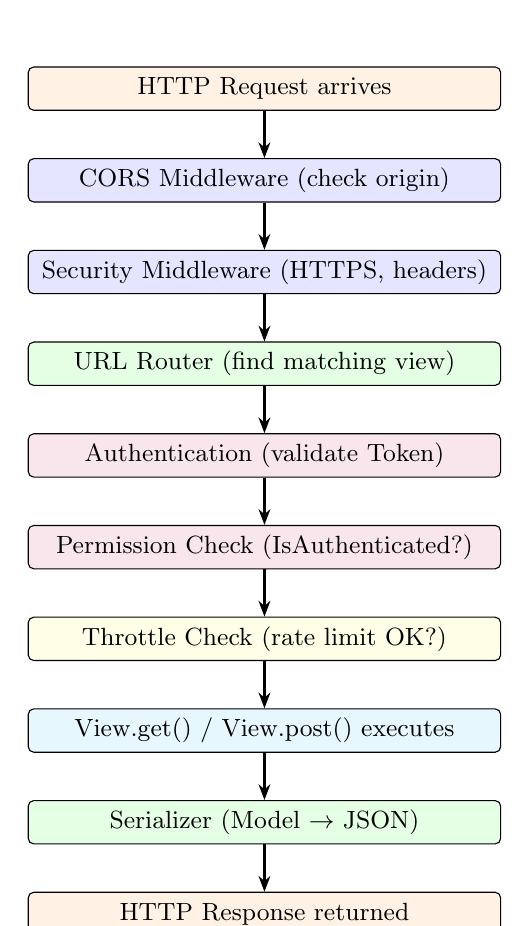
\begin{tikzpicture}[
    node distance=0.6cm,
    box/.style={rectangle, draw, rounded corners=2pt, minimum width=6cm, minimum height=0.55cm, align=center, font=\small},
    arrow/.style={-{Stealth[length=2mm]}, thick},
]
\node[box, fill=orange!10] (req) {HTTP Request arrives};
\node[box, fill=blue!10, below=of req] (cors) {CORS Middleware (check origin)};
\node[box, fill=blue!10, below=of cors] (sec) {Security Middleware (HTTPS, headers)};
\node[box, fill=green!10, below=of sec] (url) {URL Router (find matching view)};
\node[box, fill=purple!10, below=of url] (auth) {Authentication (validate Token)};
\node[box, fill=purple!10, below=of auth] (perm) {Permission Check (IsAuthenticated?)};
\node[box, fill=yellow!10, below=of perm] (throttle) {Throttle Check (rate limit OK?)};
\node[box, fill=cyan!10, below=of throttle] (view) {View.get() / View.post() executes};
\node[box, fill=green!10, below=of view] (serial) {Serializer (Model $\rightarrow$ JSON)};
\node[box, fill=orange!10, below=of serial] (resp) {HTTP Response returned};

\draw[arrow] (req) -- (cors);
\draw[arrow] (cors) -- (sec);
\draw[arrow] (sec) -- (url);
\draw[arrow] (url) -- (auth);
\draw[arrow] (auth) -- (perm);
\draw[arrow] (perm) -- (throttle);
\draw[arrow] (throttle) -- (view);
\draw[arrow] (view) -- (serial);
\draw[arrow] (serial) -- (resp);
\end{tikzpicture}
\end{center}


% ═══════════════════════════════════════════════════════════════════════
% CHAPTER 16: DEPLOYMENT
% ═══════════════════════════════════════════════════════════════════════

\chapter{Deployment \& DevOps}

\section{Docker Setup}

\begin{lstlisting}[language={},caption={Dockerfile}]
FROM python:3.11-slim
WORKDIR /app
COPY requirements.txt .
RUN pip install --no-cache-dir -r requirements.txt
COPY . .
RUN cd backend && python manage.py collectstatic --noinput
EXPOSE 8000
CMD ["python", "backend/manage.py", "runserver", "0.0.0.0:8000"]
\end{lstlisting}

\section{Environment Variables Reference}

\begin{longtable}{|p{4cm}|p{3cm}|p{6cm}|}
\hline
\textbf{Variable} & \textbf{Default} & \textbf{Purpose} \\
\hline
GROQ\_API\_KEY & (none) & Groq cloud LLM access \\
\hline
GEMINI\_API\_KEY & (none) & Google Gemini access \\
\hline
OPENAI\_API\_KEY & (none) & OpenAI GPT access \\
\hline
TAVILY\_API\_KEY & (none) & Premium web search \\
\hline
LLM\_PROVIDER & auto & Force specific provider \\
\hline
MODEL\_NAME & llama-3.3-70b & Override default model \\
\hline
MAX\_REVISIONS & 2 & Feedback loop limit \\
\hline
MAX\_SEARCH\_RESULTS & 5 & Results per query \\
\hline
CHUNK\_SIZE & 1000 & RAG chunk size (chars) \\
\hline
CHUNK\_OVERLAP & 200 & Chunk overlap (chars) \\
\hline
DJANGO\_DEBUG & True & Django debug mode \\
\hline
DJANGO\_SECRET\_KEY & (insecure) & Production secret \\
\hline
\end{longtable}


% ═══════════════════════════════════════════════════════════════════════
% CHAPTER 17: QUICK REFERENCE
% ═══════════════════════════════════════════════════════════════════════

\chapter{Quick Reference Cards}

\section{Key Numbers to Remember}

\begin{center}
\begin{tabular}{|c|l|}
\hline
\textbf{Number} & \textbf{What} \\
\hline
4 & AI Agents (Researcher, Analyst, Fact-Checker, Writer) \\
\hline
5 & LLM Providers (Groq, Gemini, OpenAI, Anthropic, Ollama) \\
\hline
2 & Search Engines (Tavily + DuckDuckGo) \\
\hline
2 & ChromaDB Collections (research\_docs + past\_research) \\
\hline
384 & Embedding dimensions (all-MiniLM-L6-v2) \\
\hline
1000/200 & Chunk size / overlap (characters) \\
\hline
18+ & REST API Endpoints \\
\hline
8 & MCP Tools \\
\hline
10 & React Components \\
\hline
62 & Unit Tests (100\% pass rate) \\
\hline
5 & Database Models \\
\hline
4 & Export Formats (MD, HTML, JSON, BibTeX) \\
\hline
3 & Architecture Layers (Frontend, Backend, AI Core) \\
\hline
2 & MAX\_REVISIONS (feedback loop limit) \\
\hline
25 & recursion\_limit (LangGraph safety) \\
\hline
15+ & Design Patterns identified \\
\hline
\end{tabular}
\end{center}

\section{Commands Cheat Sheet}

\begin{lstlisting}[language={},caption={Essential Development Commands}]
# Backend
cd backend && python manage.py runserver 0.0.0.0:8000
cd backend && python manage.py migrate
cd backend && python manage.py createsuperuser
cd backend && python -m pytest -q  # Run 62 tests

# Frontend
cd frontend && npm install
cd frontend && npm run dev  # Dev server on :5173

# MCP Server
python mcp_server.py  # Start FastMCP on stdio

# Docker
docker-compose up --build  # Start everything
\end{lstlisting}


% ═══════════════════════════════════════════════════════════════════════
% CHAPTER 18: FINAL TIPS
% ═══════════════════════════════════════════════════════════════════════

\chapter{Final Interview Tips \& Presentation Strategy}

\section{30-Second Elevator Pitch}

\begin{storybox}{Agar interviewer bole ``Tell me about your project in 30 seconds''}
``MARO ek AI-powered research platform hai jahan 4 specialized AI agents --- Researcher, Analyst, Fact-Checker, aur Writer --- collaborate karke kisi bhi topic pe verified, fact-checked research report generate karte hain. LangGraph se orchestration, ChromaDB se RAG, Django REST se API, React se UI, aur FastMCP se Claude Desktop integration. Unique feature: feedback loop jahan Fact-Checker quality issues pe Researcher ko wapas bhejta hai for re-research. 62 tests, 5 LLM providers, 18+ API endpoints.''
\end{storybox}

\section{How to Draw Architecture on Whiteboard}

\begin{enumerate}
    \item Draw 3 horizontal boxes: Frontend, Backend, AI Core
    \item In AI Core: draw 4 agent boxes in a row with arrows
    \item Add feedback loop arrow from Fact-Checker back to Researcher
    \item Add ChromaDB box to the side connected to Researcher
    \item Add ``Multi-Provider LLM'' box connected to all agents
    \item Label arrows: REST API, SSE, Python imports
    \item Add FastMCP box on the side pointing to ``Claude Desktop''
\end{enumerate}

\section{Top 5 Things Interviewers Love}

\begin{enumerate}
    \item \textbf{Feedback Loop:} Self-correcting system --- shows mature thinking
    \item \textbf{Multi-Provider Fallback:} Resilient design --- never fully fails
    \item \textbf{Benchmark Arena:} Empirical proof --- not just claims
    \item \textbf{Research Memory:} System that learns --- innovative feature
    \item \textbf{62 Tests:} Quality consciousness --- professional approach
\end{enumerate}


% ═══════════════════════════════════════════════════════════════════════
% CHAPTER 19: DRF SERIALIZERS DEEP DIVE
% ═══════════════════════════════════════════════════════════════════════

\chapter{DRF Serializers --- Data Transformation Layer}

\begin{storybox}{Serializer kya karta hai?}
Socho tum ek translator ho. Database mein data Python objects mein hai (Django Model instances). Frontend ko JSON chahiye. Toh Serializer ye kaam karta hai:

\textbf{Serialization:} Python Object $\rightarrow$ JSON (Response bhejte waqt)

\textbf{Deserialization:} JSON $\rightarrow$ Python Object (Request receive karte waqt)

Plus validation bhi karta hai --- kya incoming data correct format mein hai?
\end{storybox}

\section{All 8+ Serializers Explained}

\begin{lstlisting}[style=pythonstyle,caption={serializers.py --- UserSerializer}]
class UserSerializer(serializers.ModelSerializer):
    class Meta:
        model = User
        fields = ['id', 'username', 'email', 'date_joined']
        read_only_fields = ['id', 'date_joined']
        # id aur date_joined user modify nahi kar sakta
        # Automatically set hote hain
\end{lstlisting}

\begin{hindibox}{ModelSerializer ka Magic}
\texttt{ModelSerializer} automatically Model ke fields se serializer fields generate karta hai. Matlab ye:
\begin{lstlisting}[style=pythonstyle]
# Ye likhne ki zarurat NAHI hai:
class UserSerializer(serializers.Serializer):
    id = serializers.IntegerField(read_only=True)
    username = serializers.CharField(max_length=150)
    email = serializers.EmailField()
    date_joined = serializers.DateTimeField(read_only=True)

# ModelSerializer ye sab AUTOMATICALLY karta hai!
# Sirf model aur fields specify karo.
\end{lstlisting}
\end{hindibox}

\begin{lstlisting}[style=pythonstyle,caption={serializers.py --- RegisterSerializer with Validation}]
class RegisterSerializer(serializers.ModelSerializer):
    password = serializers.CharField(
        write_only=True,
        min_length=6,
        # write_only=True: password response mein nahi jaayega
        # Security! Password kabhi API response mein na bhejo.
    )
    email = serializers.EmailField(required=False, allow_blank=True)

    class Meta:
        model = User
        fields = ['username', 'email', 'password']

    def validate_username(self, value):
        """Custom username validation"""
        if User.objects.filter(username__iexact=value).exists():
            raise serializers.ValidationError(
                "Username already exists."
            )
        return value
        # __iexact: case-insensitive check
        # "Admin" aur "admin" same treated hain

    def create(self, validated_data):
        """Override to hash password"""
        return User.objects.create_user(**validated_data)
        # create_user() internally calls:
        #   user.set_password(password)  -> PBKDF2 hash
        # create() would store PLAINTEXT password! DANGER!
\end{lstlisting}

\begin{dangerbox}{create\_user vs create --- NEVER confuse!}
\begin{lstlisting}[style=pythonstyle]
# WRONG - stores plaintext password!
User.objects.create(username="test", password="mypass123")
# DB stores: password = "mypass123"  (HACKABLE!)

# RIGHT - hashes password with PBKDF2
User.objects.create_user(username="test", password="mypass123")
# DB stores: password = "pbkdf2_sha256$260000$salt$hash..."
# Even if DB leaked, password is safe!
\end{lstlisting}
\end{dangerbox}

\begin{lstlisting}[style=pythonstyle,caption={serializers.py --- Session Serializers (List vs Detail)}]
# === LIST VIEW: Lightweight, fast ===
class ResearchSessionListSerializer(serializers.ModelSerializer):
    user = UserSerializer(read_only=True)
    tags = serializers.SerializerMethodField()

    class Meta:
        model = ResearchSession
        fields = [
            'id', 'user', 'topic', 'status',
            'web_sources_count', 'rag_chunks_count',
            'revision_count', 'duration_seconds',
            'created_at', 'tags',
        ]
        # NOTE: final_report NOT included!
        # List view mein full report bhejne se response heavy ho jaata
        # 100 sessions * 5000 chars each = 500KB unnecessary data

    def get_tags(self, obj):
        return list(obj.tags.values_list('name', flat=True))
        # values_list('name', flat=True) returns ['AI', 'Ethics']
        # instead of [{'name': 'AI'}, {'name': 'Ethics'}]


# === DETAIL VIEW: Full data, single session ===
class ResearchSessionDetailSerializer(serializers.ModelSerializer):
    user = UserSerializer(read_only=True)
    sources = ResearchSourceSerializer(many=True, read_only=True)
    events = ResearchEventSerializer(many=True, read_only=True)
    tags = serializers.SerializerMethodField()

    class Meta:
        model = ResearchSession
        fields = '__all__'
        # __all__ = include EVERY field including final_report
        # Only used when viewing single session detail
\end{lstlisting}

\begin{conceptbox}{List vs Detail Serializer Pattern}
\textbf{Problem:} Ek hi model ke liye different views ko different data chahiye:
\begin{itemize}
    \item List view (GET /sessions/): Bahut sessions load hote hain --- lightweight data chahiye
    \item Detail view (GET /sessions/\{id\}/): Ek session ka full data chahiye --- report, sources, events sab
\end{itemize}

\textbf{Solution:} 2 separate serializers banao:
\begin{itemize}
    \item \texttt{ListSerializer}: Essential fields only (no report, no sources, no events)
    \item \texttt{DetailSerializer}: \texttt{fields = '\_\_all\_\_'} + nested sources + events
\end{itemize}

\textbf{Performance impact:}
\begin{lstlisting}[language={}]
List with DetailSerializer:  ~2.5s for 100 sessions (heavy!)
List with ListSerializer:    ~0.3s for 100 sessions (8x faster!)
\end{lstlisting}
\end{conceptbox}

\begin{lstlisting}[style=pythonstyle,caption={serializers.py --- Nested Serializers}]
class ResearchSourceSerializer(serializers.ModelSerializer):
    class Meta:
        model = ResearchSource
        fields = [
            'id', 'source_type', 'position',
            'url', 'title', 'domain', 'snippet'
        ]
        # Nested inside SessionDetailSerializer
        # sources = ResearchSourceSerializer(many=True)


class ResearchEventSerializer(serializers.ModelSerializer):
    class Meta:
        model = ResearchEvent
        fields = ['id', 'sequence', 'stage', 'message', 'created_at']


class ResearchTagSerializer(serializers.ModelSerializer):
    class Meta:
        model = ResearchTag
        fields = ['id', 'name', 'created_at']

    def validate_name(self, value):
        """Normalize tag names"""
        normalized = value.strip().lower()
        if len(normalized) < 1:
            raise serializers.ValidationError("Tag name too short")
        return normalized
        # "  AI Ethics  " -> "ai ethics"


class BenchmarkSerializer(serializers.ModelSerializer):
    class Meta:
        model = BenchmarkEvaluation
        fields = '__all__'
\end{lstlisting}

\begin{interviewbox}{Explain the difference between Serializer and ModelSerializer}
\textbf{Answer:} ``\texttt{Serializer} base class hai --- har field manually define karna padta hai: type, validators, create/update methods. \texttt{ModelSerializer} ek shortcut hai --- Model class aur fields specify karo, baaki sab auto-generate hota hai. ModelSerializer internally model introspection karta hai --- model field types (CharField, IntegerField, etc.) se corresponding serializer fields map karta hai. Plus auto-generated \texttt{create()} aur \texttt{update()} methods milte hain.

Humne ModelSerializer use kiya kyunki 5 models hain with 40+ fields total. Manually likhna = 200+ lines of boilerplate. ModelSerializer se ~50 lines mein same kaam ho gaya.

Custom validation jahan chahiye wahan \texttt{validate\_<field>()} method override kiya, jaise \texttt{validate\_username()} for case-insensitive uniqueness check.''
\end{interviewbox}


% ═══════════════════════════════════════════════════════════════════════
% CHAPTER 20: CSS DESIGN SYSTEM
% ═══════════════════════════════════════════════════════════════════════

\chapter{CSS Design System --- Visual Architecture Deep Dive}

\begin{storybox}{Design system kyun zaroori hai?}
Imagine 8 developers ek project pe kaam kar rahe hain. Ek ne button ka color \texttt{\#6366f1} rakha, doosre ne \texttt{\#6466f2} (bilkul similar but different), teesre ne \texttt{purple}. Inconsistency! Users ko lagega ki ye 3 alag alag buttons hain.

\textbf{Design System} ek ``single source of truth'' hai --- sab colors, fonts, spacings, animations ek jagah define hain. Sab components wahi use karte hain.
\end{storybox}

\section{CSS Custom Properties (Design Tokens)}

\begin{lstlisting}[style=jsstyle,caption={index.css --- Complete Design Token System}]
:root {
  /* === COLOR PALETTE === */
  --bg-primary: #050508;
  /* Almost black - premium dark background */

  --bg-secondary: #0a0a12;
  /* Slightly lighter - card backgrounds */

  --bg-tertiary: #111118;
  /* Surface elevation - input fields, modals */

  --accent-primary: #00f5f3;
  /* Cyan - primary actions, active states */
  /* High contrast on dark bg = excellent readability */

  --accent-secondary: #a855f7;
  /* Purple - secondary actions, tags, badges */

  --accent-success: #34d399;
  /* Green - success states, completed, verified */

  --accent-warning: #fbbf24;
  /* Amber - warning states, needs attention */

  --accent-danger: #f87171;
  /* Red - errors, failed states, destructive actions */

  --text-primary: #e4e4e7;
  /* Off-white - body text (not pure white = less eye strain) */

  --text-secondary: #a1a1aa;
  /* Gray - secondary text, labels, timestamps */

  --text-muted: #52525b;
  /* Dark gray - placeholders, disabled text */

  --border-default: rgba(255,255,255,0.06);
  /* Very subtle - card borders, dividers */

  --border-hover: rgba(255,255,255,0.12);
  /* Slightly visible - on hover state */

  /* === TYPOGRAPHY === */
  --font-sans: 'Inter', -apple-system, BlinkMacSystemFont, sans-serif;
  /* Inter: modern, professional, excellent readability */
  /* System font stack as fallback */

  --font-mono: 'JetBrains Mono', 'Fira Code', monospace;
  /* JetBrains Mono: designed for code readability */
  /* Ligatures for => -> !== etc. */

  /* === SPACING SCALE === */
  --space-xs: 0.25rem;    /* 4px */
  --space-sm: 0.5rem;     /* 8px */
  --space-md: 1rem;       /* 16px */
  --space-lg: 1.5rem;     /* 24px */
  --space-xl: 2rem;       /* 32px */
  --space-2xl: 3rem;      /* 48px */

  /* === BORDER RADIUS === */
  --radius-sm: 6px;
  --radius-md: 10px;
  --radius-lg: 16px;
  --radius-xl: 24px;

  /* === SHADOWS === */
  --shadow-card: 0 4px 24px rgba(0,0,0,0.3);
  --shadow-glow: 0 0 20px rgba(0,245,243,0.15);
  /* Cyan glow effect for active elements */

  /* === TRANSITIONS === */
  --transition-fast: 150ms ease;
  --transition-normal: 250ms ease;
  --transition-slow: 400ms cubic-bezier(0.4,0,0.2,1);
}
\end{lstlisting}

\begin{conceptbox}{Why CSS Custom Properties over Hardcoded Values?}
\begin{lstlisting}[style=jsstyle]
/* BAD: Hardcoded everywhere */
.button { background: #6366f1; }
.badge  { background: #6366f1; }
.link   { color: #6366f1; }
/* Want to change accent? Update 50+ places! */

/* GOOD: Design tokens */
.button { background: var(--accent-primary); }
.badge  { background: var(--accent-primary); }
.link   { color: var(--accent-primary); }
/* Change accent? Update ONE place in :root! */
\end{lstlisting}

\textbf{Bonus:} CSS variables are runtime-changeable. Theme switching just needs:
\begin{lstlisting}[style=jsstyle]
document.documentElement.style.setProperty(
  '--accent-primary', '#ff6b6b'  // Red theme!
);
// All components update instantly! No page reload.
\end{lstlisting}
\end{conceptbox}

\section{Component-Level Styles}

\begin{lstlisting}[style=jsstyle,caption={index.css --- Button System}]
/* === BASE BUTTON === */
.btn {
  display: inline-flex;
  align-items: center;
  gap: var(--space-sm);
  padding: var(--space-sm) var(--space-lg);
  border-radius: var(--radius-md);
  font-family: var(--font-sans);
  font-weight: 600;
  font-size: 0.875rem;
  cursor: pointer;
  transition: all var(--transition-normal);
  border: 1px solid transparent;
  text-decoration: none;
  white-space: nowrap;
}

/* === PRIMARY VARIANT === */
.btn-primary {
  background: linear-gradient(135deg,
    var(--accent-primary),
    var(--accent-secondary));
  /* Gradient: cyan -> purple = premium look */
  color: #000;
  /* Dark text on light gradient for contrast */
  box-shadow: var(--shadow-glow);
}

.btn-primary:hover {
  transform: translateY(-2px);
  /* Subtle lift on hover = depth feedback */
  box-shadow: 0 0 30px rgba(0,245,243,0.3);
  /* Intensified glow */
  filter: brightness(1.1);
  /* Slightly brighter */
}

.btn-primary:active {
  transform: translateY(0);
  /* Press down = satisfying click feedback */
}

.btn-primary:disabled {
  opacity: 0.5;
  cursor: not-allowed;
  transform: none;
  box-shadow: none;
}

/* === GHOST VARIANT === */
.btn-ghost {
  background: transparent;
  color: var(--text-secondary);
  border: 1px solid var(--border-default);
}

.btn-ghost:hover {
  background: rgba(255,255,255,0.05);
  border-color: var(--border-hover);
  color: var(--text-primary);
}
\end{lstlisting}

\begin{lstlisting}[style=jsstyle,caption={index.css --- Glass Card System}]
/* === GLASSMORPHISM CARD === */
.glass-card {
  background: rgba(10, 10, 18, 0.7);
  /* Semi-transparent dark background */
  backdrop-filter: blur(12px);
  /* Blur content behind the card */
  -webkit-backdrop-filter: blur(12px);
  /* Safari support */
  border: 1px solid var(--border-default);
  border-radius: var(--radius-lg);
  padding: var(--space-lg);
  box-shadow: var(--shadow-card);
}

.glass-card:hover {
  border-color: var(--border-hover);
  box-shadow: var(--shadow-card),
              0 0 40px rgba(0,245,243,0.05);
  /* Subtle glow on hover */
}

/* === STREAMING TERMINAL === */
.terminal {
  background: #0a0a0f;
  border: 1px solid rgba(0,245,243,0.15);
  border-radius: var(--radius-md);
  font-family: var(--font-mono);
  font-size: 0.8rem;
  line-height: 1.6;
  padding: var(--space-md);
  max-height: 400px;
  overflow-y: auto;
  scroll-behavior: smooth;
}

.terminal-line {
  padding: 2px 0;
  display: flex;
  gap: var(--space-sm);
}

.terminal-timestamp {
  color: var(--text-muted);
  font-size: 0.7rem;
  min-width: 80px;
}

.terminal-message {
  color: var(--accent-primary);
}

/* === ANIMATIONS === */
@keyframes pulse-glow {
  0%, 100% { box-shadow: 0 0 5px rgba(0,245,243,0.2); }
  50%      { box-shadow: 0 0 20px rgba(0,245,243,0.4); }
}

@keyframes slide-in {
  from { opacity: 0; transform: translateY(10px); }
  to   { opacity: 1; transform: translateY(0); }
}

.agent-active {
  animation: pulse-glow 2s ease-in-out infinite;
}

.fade-in {
  animation: slide-in 0.3s ease-out forwards;
}
\end{lstlisting}

\begin{interviewbox}{Explain your CSS architecture decisions}
\textbf{Answer:} ``Design system approach use kiya with CSS Custom Properties as design tokens. :root mein sab colors, fonts, spacings, radii, shadows define hain --- components mein var() se reference karte hain. Benefits: (1) Global consistency --- ek color change karo, sab jagah update. (2) Theme-ability --- dark/light mode switching possible. (3) No class name collisions --- BEM-inspired naming.

Premium look ke liye: glassmorphism (backdrop-filter: blur), gradient buttons, cyan glow effects (@keyframes pulse-glow), micro-animations (translateY on hover for depth), aur monospace JetBrains Mono font for terminal.

Accessibility: off-white text (#e4e4e7) instead of pure white for reduced eye strain on dark background. WCAG AA contrast ratios maintained. Focus-visible states for keyboard navigation.''
\end{interviewbox}


% ═══════════════════════════════════════════════════════════════════════
% CHAPTER 21: FRONTEND COMPONENTS DEEP DIVE
% ═══════════════════════════════════════════════════════════════════════

\chapter{Frontend Components --- Every Component Explained}

\section{App.jsx --- Root Component with Tab Routing}

\begin{lstlisting}[style=jsstyle,caption={App.jsx --- Application Shell}]
import { useState, useEffect, useCallback } from 'react';
import { api } from './api';
import Navbar from './components/Navbar';
import AuthModal from './components/AuthModal';
import ResearchStudio from './components/ResearchStudio';
import LibraryView from './components/LibraryView';
import RAGHubView from './components/RAGHubView';
import BenchmarkArenaView from './components/BenchmarkArenaView';
import LLMMCPHubView from './components/LLMMCPHubView';

export default function App() {
  const [activeTab, setActiveTab] = useState('studio');
  // Which tab is currently shown

  const [user, setUser] = useState(null);
  // Logged in user object (null = not logged in)

  const [showAuth, setShowAuth] = useState(false);
  // Is the login/register modal visible?

  const [backendAlive, setBackendAlive] = useState(false);
  // Is Django server reachable?

  // === AUTO-LOGIN ON PAGE LOAD ===
  useEffect(() => {
    const token = localStorage.getItem('maro_auth_token');
    if (token) {
      api.getProfile()
        .then(data => setUser(data.user || data))
        .catch(() => {
          // Token expired or invalid
          localStorage.removeItem('maro_auth_token');
        });
    }
  }, []);
  // [] dependency array = run ONCE on mount

  // === HEALTH CHECK ===
  useEffect(() => {
    api.healthCheck()
      .then(() => setBackendAlive(true))
      .catch(() => setBackendAlive(false));
  }, []);

  // === LOGIN/LOGOUT HANDLERS ===
  const handleLogin = useCallback((userData, token) => {
    setUser(userData);
    api.setToken(token);
    setShowAuth(false);
  }, []);
  // useCallback prevents unnecessary re-renders of child components

  const handleLogout = useCallback(() => {
    api.logout();
    setUser(null);
  }, []);

  // === TAB CONTENT RENDERING ===
  const renderTabContent = () => {
    switch (activeTab) {
      case 'studio':
        return <ResearchStudio user={user} />;
      case 'library':
        return <LibraryView user={user} />;
      case 'rag':
        return <RAGHubView />;
      case 'benchmark':
        return <BenchmarkArenaView />;
      case 'llm':
        return <LLMMCPHubView />;
      default:
        return <ResearchStudio user={user} />;
    }
  };

  return (
    <div className="app-container">
      <Navbar
        activeTab={activeTab}
        onTabChange={setActiveTab}
        user={user}
        backendAlive={backendAlive}
        onLoginClick={() => setShowAuth(true)}
        onLogout={handleLogout}
      />

      <main className="main-content">
        {renderTabContent()}
      </main>

      {showAuth && (
        <AuthModal
          onLogin={handleLogin}
          onClose={() => setShowAuth(false)}
        />
      )}
    </div>
  );
}
\end{lstlisting}

\begin{conceptbox}{Tab-Based Routing vs React Router}
\textbf{Question:} React Router kyun nahi use kiya?

\textbf{Answer:} ``MARO ek single-page dashboard hai, not a multi-page website. Saare ``pages'' actually tabs hain jo ek hi page pe render hote hain. Benefits: (1) No URL changes = no browser history pollution. (2) Tab state preserved --- agar Library tab pe search kiya, Studio tab pe research kiya, phir Library pe wapas aaye toh search results preserved hain (component unmount nahi hua). (3) Simpler code --- useState vs react-router-dom setup.

Agar ye ek public-facing site hoti with shareable URLs (e.g., /research/123), toh React Router use karta with route params.''
\end{conceptbox}

\section{AuthModal --- Login/Register with Validation}

\begin{lstlisting}[style=jsstyle,caption={AuthModal.jsx --- Dual-Mode Authentication}]
export default function AuthModal({ onLogin, onClose }) {
  const [isRegister, setIsRegister] = useState(false);
  // false = login mode, true = register mode

  const [form, setForm] = useState({
    username: '', email: '', password: ''
  });
  const [loading, setLoading] = useState(false);
  const [error, setError] = useState('');

  const handleSubmit = async (e) => {
    e.preventDefault();
    // ^^ Prevent form default submission (page reload)
    setLoading(true);
    setError('');

    try {
      let data;
      if (isRegister) {
        data = await api.register(
          form.username, form.email, form.password
        );
      } else {
        data = await api.login(form.username, form.password);
      }
      onLogin(data.user, data.token);
      // Parent component stores user + token

    } catch (err) {
      setError(err.message || 'Something went wrong');
    } finally {
      setLoading(false);
      // Always stop loading spinner, even on error
    }
  };

  return (
    // Modal overlay with backdrop
    <div className="modal-overlay" onClick={onClose}>
      <div className="glass-card modal-card"
           onClick={e => e.stopPropagation()}>
        {/* ^^ stopPropagation: clicking inside modal
            shouldn't close it (only backdrop click closes) */}

        <h2>{isRegister ? 'Create Account' : 'Sign In'}</h2>

        {error && (
          <div className="error-banner">{error}</div>
        )}

        <form onSubmit={handleSubmit}>
          <input
            type="text"
            placeholder="Username"
            value={form.username}
            onChange={e => setForm({
              ...form, username: e.target.value
            })}
            required
            autoFocus
          />

          {isRegister && (
            <input type="email" placeholder="Email (optional)"
                   value={form.email}
                   onChange={e => setForm({
                     ...form, email: e.target.value
                   })} />
          )}

          <input type="password" placeholder="Password"
                 value={form.password}
                 onChange={e => setForm({
                   ...form, password: e.target.value
                 })}
                 required minLength={6} />

          <button type="submit" className="btn btn-primary"
                  disabled={loading}>
            {loading ? 'Processing...'
                     : isRegister ? 'Register' : 'Login'}
          </button>
        </form>

        <p className="toggle-text">
          {isRegister ? 'Already have an account?' : 'New here?'}
          <button onClick={() => setIsRegister(!isRegister)}>
            {isRegister ? 'Sign In' : 'Create Account'}
          </button>
        </p>
      </div>
    </div>
  );
}
\end{lstlisting}

\section{LibraryView --- Session History with Search}

\begin{lstlisting}[style=jsstyle,caption={LibraryView.jsx --- Search and Filter Logic}]
export default function LibraryView({ user }) {
  const [sessions, setSessions] = useState([]);
  const [searchQuery, setSearchQuery] = useState('');
  const [statusFilter, setStatusFilter] = useState('all');
  const [loading, setLoading] = useState(true);
  const [expandedId, setExpandedId] = useState(null);

  // === LOAD SESSIONS ===
  const loadSessions = useCallback(async () => {
    try {
      setLoading(true);
      const data = await api.getSessions();
      setSessions(data.results || data || []);
    } catch (err) {
      console.error('Failed to load sessions:', err);
    } finally {
      setLoading(false);
    }
  }, []);

  useEffect(() => { loadSessions(); }, [loadSessions]);

  // === CLIENT-SIDE FILTERING ===
  const filteredSessions = sessions.filter(s => {
    const matchesSearch = searchQuery === ''
      || s.topic.toLowerCase().includes(
           searchQuery.toLowerCase()
         );
    // Case-insensitive topic search

    const matchesStatus = statusFilter === 'all'
      || s.status === statusFilter;

    return matchesSearch && matchesStatus;
  });

  // === DELETE SESSION ===
  const handleDelete = async (id) => {
    if (!window.confirm('Delete this research session?')) return;
    try {
      await api.deleteSession(id);
      setSessions(prev => prev.filter(s => s.id !== id));
      // Optimistic UI: remove from list immediately
      // Don't wait for server confirmation
    } catch (err) {
      alert('Failed to delete: ' + err.message);
    }
  };

  // === EXPORT ===
  const handleExport = async (id, format) => {
    const url = `${API_BASE}/research/sessions/${id}/export/` +
                `?format=${format}`;
    window.open(url, '_blank');
    // Opens in new tab -> browser handles download
  };

  return (
    <div className="library-container">
      {/* Search + Filter Bar */}
      <div className="filter-bar">
        <input type="text" placeholder="Search topics..."
               value={searchQuery}
               onChange={e => setSearchQuery(e.target.value)} />

        <select value={statusFilter}
                onChange={e => setStatusFilter(e.target.value)}>
          <option value="all">All Status</option>
          <option value="completed">Completed</option>
          <option value="running">Running</option>
          <option value="failed">Failed</option>
        </select>
      </div>

      {/* Session Cards */}
      {filteredSessions.map(session => (
        <div key={session.id} className="glass-card session-card">
          <h3>{session.topic}</h3>
          <div className="session-meta">
            <span className={`status-badge ${session.status}`}>
              {session.status}
            </span>
            <span>{session.web_sources_count} sources</span>
            <span>{session.revision_count} revisions</span>
            <span>
              {new Date(session.created_at).toLocaleDateString()}
            </span>
          </div>

          {/* Expandable Report Preview */}
          {expandedId === session.id && (
            <div className="report-preview"
                 dangerouslySetInnerHTML={{
                   __html: marked.parse(
                     session.final_report || 'No report'
                   )
                 }} />
          )}

          <div className="session-actions">
            <button onClick={() => setExpandedId(
              expandedId === session.id ? null : session.id
            )}>
              {expandedId === session.id ? 'Collapse' : 'Expand'}
            </button>
            <button onClick={() => handleExport(session.id, 'markdown')}>
              Export MD
            </button>
            <button onClick={() => handleDelete(session.id)}>
              Delete
            </button>
          </div>
        </div>
      ))}
    </div>
  );
}
\end{lstlisting}

\section{RAGHubView --- Vector Store Management}

\begin{lstlisting}[style=jsstyle,caption={RAGHubView.jsx --- Document Upload + Search}]
export default function RAGHubView() {
  const [stats, setStats] = useState(null);
  const [uploading, setUploading] = useState(false);
  const [searchQuery, setSearchQuery] = useState('');
  const [searchResults, setSearchResults] = useState([]);
  const fileInputRef = useRef(null);

  // Load collection stats on mount
  useEffect(() => {
    api.ragStats().then(setStats).catch(console.error);
  }, []);

  // === FILE UPLOAD ===
  const handleUpload = async (e) => {
    const files = Array.from(e.target.files);
    if (!files.length) return;

    setUploading(true);
    const formData = new FormData();
    files.forEach(f => formData.append('documents', f));
    // FormData allows file upload via HTTP
    // 'documents' matches Django's request.FILES key

    try {
      const result = await api.uploadDocuments(formData);
      // Refresh stats after upload
      const newStats = await api.ragStats();
      setStats(newStats);
      alert(`Uploaded! ${result.chunks_added} chunks indexed.`);
    } catch (err) {
      alert('Upload failed: ' + err.message);
    } finally {
      setUploading(false);
    }
  };

  // === SEMANTIC SEARCH ===
  const handleSearch = async () => {
    if (!searchQuery.trim()) return;
    try {
      const results = await api.ragSearch(searchQuery);
      setSearchResults(results);
    } catch (err) {
      console.error('RAG search failed:', err);
    }
  };

  return (
    <div className="rag-hub">
      {/* Stats Cards */}
      {stats && (
        <div className="stats-grid">
          <div className="glass-card stat-card">
            <h4>Research Docs</h4>
            <span className="stat-number">
              {stats.research_docs || 0}
            </span>
            <span className="stat-label">chunks indexed</span>
          </div>
          <div className="glass-card stat-card">
            <h4>Past Research</h4>
            <span className="stat-number">
              {stats.past_research || 0}
            </span>
            <span className="stat-label">memory chunks</span>
          </div>
        </div>
      )}

      {/* Upload Section */}
      <div className="glass-card upload-zone"
           onClick={() => fileInputRef.current?.click()}>
        <input ref={fileInputRef} type="file"
               accept=".pdf" multiple hidden
               onChange={handleUpload} />
        <p>{uploading ? 'Uploading...'
                      : 'Click to upload PDFs'}</p>
      </div>

      {/* Semantic Search */}
      <div className="glass-card search-section">
        <h3>Semantic Search</h3>
        <div className="search-bar">
          <input value={searchQuery}
                 onChange={e => setSearchQuery(e.target.value)}
                 placeholder="Search your knowledge base..."
                 onKeyDown={e => e.key === 'Enter'
                            && handleSearch()} />
          <button onClick={handleSearch}>Search</button>
        </div>
        {searchResults.map((r, i) => (
          <div key={i} className="search-result glass-card">
            <p>{r.content}</p>
            <small>Score: {r.score?.toFixed(3)}</small>
          </div>
        ))}
      </div>
    </div>
  );
}
\end{lstlisting}


% ═══════════════════════════════════════════════════════════════════════
% CHAPTER 22: ADVANCED INTERVIEW Q&A --- PART 2
% ═══════════════════════════════════════════════════════════════════════

\chapter{Advanced Interview Q\&A --- Part 2 (30+ More Questions)}

\section{LangChain \& LangGraph Deep Dive}

\begin{interviewbox}{What is the difference between LangChain and LangGraph?}
\textbf{Answer:} ``LangChain ek LLM application framework hai --- chains, prompts, tools, memory, retrievers provide karta hai. Ye building blocks hain. LangGraph LangChain ke upar built hai --- ye specifically \textbf{stateful, multi-actor} applications ke liye hai. Key difference: LangChain mein chains linear hain (A $\rightarrow$ B $\rightarrow$ C). LangGraph mein \textbf{conditional edges} aur \textbf{cycles} possible hain --- matlab loops, branches, parallel execution. MARO mein humara feedback loop (Fact-Checker $\rightarrow$ Researcher) plain LangChain mein directly possible nahi tha --- LangGraph ka conditional edge ye enable karta hai.''
\end{interviewbox}

\begin{interviewbox}{What is a StateGraph vs MessageGraph?}
\textbf{Answer:} ``LangGraph mein 2 graph types hain: \texttt{MessageGraph} sirf messages (chat-like) handle karta hai --- simple chatbots ke liye. \texttt{StateGraph} arbitrary typed state handle karta hai --- TypedDict with custom fields. Humne StateGraph use kiya kyunki humein sirf messages nahi chahiye --- research\_data, analysis, fact\_check\_result, revision\_count sab custom fields hain jo graph ke through flow karte hain. StateGraph zyada flexible hai --- koi bhi Python type state mein rakh sakte ho.''
\end{interviewbox}

\begin{interviewbox}{What is graph compilation and why is it needed?}
\textbf{Answer:} ``\texttt{workflow.compile()} call se CompiledGraph object banta hai. Compilation mein: (1) Graph structure validate hota hai --- kya sab nodes reachable hain? Kya cycles mein exit condition hai? (2) Execution plan optimize hota hai --- node order determine hota hai. (3) State reducers wire up hote hain --- kaunsa field accumulate karega, kaunsa replace. Compiled graph thread-safe hai --- multiple requests same compiled graph instance pe safely run ho sakte hain kyunki har invocation apna independent state copy banata hai.''
\end{interviewbox}

\section{Database \& ORM Questions}

\begin{interviewbox}{Why denormalized counters instead of COUNT queries?}
\textbf{Answer:} ``List view mein 100 sessions load hote hain. Agar har session ke liye web\_sources\_count calculate karein: \texttt{session.sources.filter(source\_type='web').count()} --- ye 100 additional SQL queries hain (N+1 problem)! Denormalized counter se: \texttt{session.web\_sources\_count} --- zero extra queries, value already in session row. Trade-off: write complexity badhti hai --- har source create hone pe counter increment karna padta hai. But reads 100x zyada hain writes se, toh ye correct trade-off hai.''
\end{interviewbox}

\begin{interviewbox}{Explain the N+1 query problem and how you handle it}
\textbf{Answer:} ``N+1 problem: 1 query for sessions + N queries for each session's related data.

\textbf{Example of N+1:}
\begin{lstlisting}[style=pythonstyle]
sessions = ResearchSession.objects.all()  # 1 query
for s in sessions:
    print(s.sources.count())  # N queries!
# Total: N+1 queries. For 100 sessions = 101 queries!
\end{lstlisting}

\textbf{Solutions used in MARO:}

(1) \textbf{Denormalized counters:} web\_sources\_count field on session itself.

(2) \textbf{select\_related():} For ForeignKey joins:
\begin{lstlisting}[style=pythonstyle]
sessions = ResearchSession.objects.select_related('user')
# 1 query with SQL JOIN instead of N separate user lookups
\end{lstlisting}

(3) \textbf{prefetch\_related():} For reverse ForeignKey / M2M:
\begin{lstlisting}[style=pythonstyle]
sessions = ResearchSession.objects.prefetch_related('sources')
# 2 queries total: 1 for sessions + 1 for ALL their sources
\end{lstlisting}

(4) \textbf{Separate serializers:} List serializer doesn't include nested sources/events at all --- no need to load them.''
\end{interviewbox}

\begin{interviewbox}{What is on\_delete=CASCADE and alternatives?}
\textbf{Answer:} ``\texttt{on\_delete} defines behavior when referenced object is deleted.
\begin{itemize}
    \item \textbf{CASCADE:} Delete parent $\rightarrow$ delete all children. Used: User deleted $\rightarrow$ all their sessions deleted.
    \item \textbf{PROTECT:} Prevent parent deletion if children exist. Used when data loss is unacceptable.
    \item \textbf{SET\_NULL:} Set FK to NULL on parent deletion. Requires null=True.
    \item \textbf{SET\_DEFAULT:} Set FK to default value.
    \item \textbf{DO\_NOTHING:} Database-level constraint only. Can cause IntegrityError.
\end{itemize}
MARO mein CASCADE use kiya kyunki sessions are user-owned --- user delete hone pe unke sessions ka koi matlab nahi rehta.''
\end{interviewbox}

\section{Frontend / React Questions}

\begin{interviewbox}{Explain useCallback and when to use it}
\textbf{Answer:} ``\texttt{useCallback} ek function ko memoize karta hai --- re-render pe same function reference return karta hai (jab tak dependencies change na hon).

\textbf{Without useCallback:}
\begin{lstlisting}[style=jsstyle]
function App() {
  const loadSessions = async () => { ... };
  // ^^ NEW function object created on EVERY render
  // Child component receiving this as prop will re-render too!

  useEffect(() => { loadSessions(); }, [loadSessions]);
  // ^^ INFINITE LOOP! loadSessions changes every render
  //    -> effect runs -> state changes -> re-render
  //    -> loadSessions changes -> effect runs -> ...
}
\end{lstlisting}

\textbf{With useCallback:}
\begin{lstlisting}[style=jsstyle]
function App() {
  const loadSessions = useCallback(async () => { ... }, []);
  // ^^ SAME function reference across renders
  // [] = never changes (no dependencies)

  useEffect(() => { loadSessions(); }, [loadSessions]);
  // ^^ Runs ONCE on mount, not infinite loop
}
\end{lstlisting}

MARO mein useCallback API loaders ke liye use kiya --- useEffect dependency arrays ko stable rakhne ke liye.''
\end{interviewbox}

\begin{interviewbox}{What is dangerouslySetInnerHTML and its risks?}
\textbf{Answer:} ``React by default HTML strings ko escape karta hai (XSS prevention). \texttt{dangerouslySetInnerHTML} raw HTML inject karta hai --- name mein `dangerous' isliye hai kyunki XSS attack possible hai.

MARO mein use: \texttt{marked.parse(report)} Markdown ko HTML mein convert karta hai, phir \texttt{dangerouslySetInnerHTML} se render hota hai.

\textbf{Risk:} Agar report mein malicious \texttt{<script>} tag ho toh XSS attack.

\textbf{Mitigation:} (1) marked.js by default scripts sanitize karta hai. (2) Report content LLM se aata hai, user-generated nahi hai. (3) Production mein DOMPurify library use karke double-sanitize karna recommend karunga.''
\end{interviewbox}

\begin{interviewbox}{How does auto-scroll work in the streaming terminal?}
\textbf{Answer:} ``Terminal ke bottom mein ek invisible div hai with useRef:

\begin{lstlisting}[style=jsstyle]
const terminalBottomRef = useRef(null);

useEffect(() => {
  terminalBottomRef.current?.scrollIntoView({
    behavior: 'smooth'
  });
}, [events]);
// ^^ events change -> scroll to bottom
// behavior: 'smooth' -> animated scroll, not jump

// In JSX:
<div className="terminal">
  {events.map(e => <div>{e.message}</div>)}
  <div ref={terminalBottomRef} />
  {/* ^^ invisible anchor at bottom */}
</div>
\end{lstlisting}

\texttt{scrollIntoView()} browser API hai --- element ko visible viewport mein scroll karta hai. Smooth behavior CSS animation lagata hai for pleasant UX.''
\end{interviewbox}

\section{Security Questions}

\begin{interviewbox}{How do you prevent CSRF attacks?}
\textbf{Answer:} ``Token Authentication inherently CSRF-resistant hai! CSRF attacks cookies pe depend karte hain --- browser automatically cookie attach karta hai every request pe. But humara auth token \texttt{Authorization: Token xxx} header mein hai jo manually set hota hai --- browser ye automatically nahi bhejta. Toh attacker ka malicious form humara token send nahi kar payega.

SessionAuthentication ke liye Django CSRF middleware active hai --- @csrf\_exempt sirf specific views pe use kiya hai (jahan token auth primary hai).''
\end{interviewbox}

\begin{interviewbox}{How is password stored securely?}
\textbf{Answer:} ``Django default: PBKDF2-SHA256 with random salt. Password kabhi plaintext store nahi hota:

\begin{lstlisting}[language={}]
Stored: pbkdf2_sha256$260000$salt$hash

Components:
- Algorithm: PBKDF2 with SHA-256
- Iterations: 260,000 (brute-force resistant)
- Salt: Random per-user (rainbow table resistant)
- Hash: Final derived key

Verification: hash(input + stored_salt) == stored_hash
\end{lstlisting}

Even if database leak ho jaaye, passwords safe hain --- attacker ko 260,000 iterations per guess try karne padenge per password. Salting ensures same password different users ke liye different hash produce karta hai.''
\end{interviewbox}

\begin{interviewbox}{What is rate limiting and how did you implement it?}
\textbf{Answer:} ``Rate limiting = requests per time window limit. DRF built-in throttle classes use kiye:
\begin{lstlisting}[style=pythonstyle]
'DEFAULT_THROTTLE_RATES': {
    'anon': '30/minute',     # Unauthenticated
    'user': '120/minute',    # Authenticated
}
\end{lstlisting}

DRF internally request count track karta hai (in-memory cache by default, Redis recommended for production). 31st anonymous request within 1 minute pe 429 Too Many Requests response aata hai with Retry-After header.

\textbf{Why different rates?} Anonymous users = potential attackers. Authenticated users identified hain --- zyada rate allowed. Also, research pipeline expensive hai (LLM calls + web search), toh rate limiting prevents abuse.''
\end{interviewbox}

\section{System Design \& Scaling Questions}

\begin{interviewbox}{How would you scale MARO to handle 1000 concurrent users?}
\textbf{Answer:} ``Current architecture ke 4 bottlenecks hain aur unke solutions:

\textbf{Bottleneck 1: SQLite} --- single-writer lock. \\
\textbf{Solution:} PostgreSQL with connection pooling (pgbouncer). Supports concurrent reads/writes.

\textbf{Bottleneck 2: threading.Thread} --- no queue, no retry, no monitoring. \\
\textbf{Solution:} Celery + Redis. Celery provides: distributed task queue, automatic retries, monitoring dashboard (Flower), horizontal scaling (add more workers), task priorities.

\textbf{Bottleneck 3: Single Django process} --- one machine. \\
\textbf{Solution:} Gunicorn with multiple workers behind Nginx. Docker + Kubernetes for auto-scaling. Load balancer distributes requests.

\textbf{Bottleneck 4: LLM API rate limits} --- Groq has per-minute token limits. \\
\textbf{Solution:} Multi-provider already handles this partially. Additionally: request queuing with backpressure, per-user quotas, provider-level rate limit tracking with token bucket algorithm.''
\end{interviewbox}

\begin{interviewbox}{What would you add if you had 2 more months?}
\textbf{Answer:} ``Priority order:
\begin{enumerate}
    \item \textbf{Celery + Redis:} Proper job queue --- most impactful for reliability
    \item \textbf{User feedback loop:} Users rate report quality $\rightarrow$ improve prompts
    \item \textbf{Citation verification:} Validate source URLs are actually reachable
    \item \textbf{Collaborative research:} Multiple users work on same topic
    \item \textbf{Agent customization:} Users can modify agent prompts and behavior
    \item \textbf{Multi-language reports:} Reports in Hindi, Spanish, etc.
    \item \textbf{Scheduled research:} Daily automated research on subscribed topics
    \item \textbf{GraphQL API:} Flexible querying instead of fixed REST endpoints
\end{enumerate}''
\end{interviewbox}


% ═══════════════════════════════════════════════════════════════════════
% CHAPTER 23: COMPLETE CODE WALKTHROUGHS
% ═══════════════════════════════════════════════════════════════════════

\chapter{Complete Code Walkthroughs --- Line by Line}

\section{Django URL Configuration}

\begin{lstlisting}[style=pythonstyle,caption={backend/api/urls.py --- All URL Patterns}]
from django.urls import path
from . import views

urlpatterns = [
    # === HEALTH ===
    path("health/",
         views.HealthAPIView.as_view()),
    # GET -> returns {"status": "ok", "provider": "groq"}

    # === AUTHENTICATION ===
    path("auth/register/",
         views.RegisterAPIView.as_view()),
    path("auth/login/",
         views.LoginAPIView.as_view()),
    path("auth/logout/",
         views.LogoutAPIView.as_view()),
    path("auth/profile/",
         views.ProfileAPIView.as_view()),
    path("auth/change-password/",
         views.ChangePasswordAPIView.as_view()),

    # === RESEARCH PIPELINE ===
    path("research/execute/",
         views.ResearchExecuteAPIView.as_view()),
    # ^^ Legacy synchronous endpoint
    path("research/stream/",
         views.ResearchStreamAPIView.as_view()),
    # ^^ SSE streaming endpoint
    path("research/jobs/",
         views.ResearchJobsAPIView.as_view()),
    # ^^ GET: list jobs, POST: create job

    # === DOCUMENT MANAGEMENT ===
    path("research/documents/",
         views.DocumentUploadAPIView.as_view()),
    # ^^ POST with multipart/form-data

    # === SESSION CRUD ===
    path("research/sessions/",
         views.SessionListAPIView.as_view()),
    path("research/sessions/<int:pk>/",
         views.SessionDetailAPIView.as_view()),
    # ^^ <int:pk> = integer primary key from URL
    path("research/sessions/<int:pk>/export/",
         views.ExportReportAPIView.as_view()),

    # === TAGS ===
    path("research/<int:pk>/tags/",
         views.ResearchTagsAPIView.as_view()),
    # ^^ GET: list tags, POST: add tag

    # === BENCHMARKING ===
    path("research/benchmark/",
         views.BenchmarkAPIView.as_view()),
    path("benchmark/history/",
         views.BenchmarkHistoryAPIView.as_view()),

    # === ANALYTICS ===
    path("stats/",
         views.PlatformStatsAPIView.as_view()),
    path("rag/stats/",
         views.RAGStatsAPIView.as_view()),
    path("rag/search/",
         views.RAGSearchAPIView.as_view()),
]
\end{lstlisting}

\begin{hindibox}{URL Pattern Anatomy}
\begin{lstlisting}[style=pythonstyle]
path("research/sessions/<int:pk>/", view)
#     ^^^^^^^^^^^^^^^^^^^^^^^^^^^^^^
#     |        |             |    |
#     |        |             |    +-- Trailing slash (Django convention)
#     |        |             +------- pk variable (integer type)
#     |        +--------------------- URL segment
#     +------------------------------ URL prefix (from root urls.py)

# When URL is: /api/research/sessions/42/
# Django sets: kwargs = {"pk": 42}
# View receives: self.kwargs["pk"] = 42
\end{lstlisting}
\end{hindibox}

\section{Django Views Deep Dive}

\begin{lstlisting}[style=pythonstyle,caption={views.py --- Health Check with Provider Info}]
class HealthAPIView(APIView):
    permission_classes = [permissions.AllowAny]
    # No auth needed - used by frontend to check if backend is alive

    def get(self, request):
        try:
            from config.providers import (
                active_provider, active_model
            )
            provider = active_provider()
            model = active_model()
        except Exception:
            provider = "unknown"
            model = "unknown"

        return Response({
            "status": "ok",
            "provider": provider,
            "model": model,
            "timestamp": timezone.now().isoformat(),
            "version": "2.0.0",
        })
\end{lstlisting}

\begin{lstlisting}[style=pythonstyle,caption={views.py --- Platform Statistics}]
class PlatformStatsAPIView(APIView):
    permission_classes = [permissions.AllowAny]

    def get(self, request):
        from django.db.models import Avg, Count

        sessions = ResearchSession.objects.all()
        total = sessions.count()
        completed = sessions.filter(status="completed").count()
        failed = sessions.filter(status="failed").count()

        # Average research duration
        avg_duration = sessions.filter(
            duration_seconds__isnull=False
        ).aggregate(
            avg=Avg("duration_seconds")
        )["avg"] or 0

        # Average sources per session
        avg_sources = sessions.filter(
            web_sources_count__gt=0
        ).aggregate(
            avg=Avg("web_sources_count")
        )["avg"] or 0

        # Revision statistics
        revision_sessions = sessions.filter(
            revision_count__gt=0
        ).count()

        return Response({
            "total_sessions": total,
            "completed": completed,
            "failed": failed,
            "success_rate": round(
                (completed / total * 100) if total > 0 else 0, 1
            ),
            "avg_duration_seconds": round(avg_duration, 1),
            "avg_sources": round(avg_sources, 1),
            "sessions_with_revisions": revision_sessions,
            "revision_rate": round(
                (revision_sessions / total * 100)
                if total > 0 else 0, 1
            ),
        })
\end{lstlisting}

\section{Vite Configuration}

\begin{lstlisting}[style=jsstyle,caption={vite.config.js --- Build Configuration}]
import { defineConfig } from 'vite';
import react from '@vitejs/plugin-react';

export default defineConfig({
  plugins: [react()],
  // react() plugin enables:
  // - JSX transformation
  // - Fast Refresh (HMR for React components)
  // - React-specific optimizations

  server: {
    port: 5173,
    // Default Vite dev server port
    proxy: {
      '/api': {
        target: 'http://localhost:8000',
        changeOrigin: true,
      }
      // During development:
      // Frontend at :5173, Backend at :8000
      // Proxy /api/* requests to Django
      // No CORS issues! Same-origin from browser's perspective
    }
  },

  build: {
    outDir: 'dist',
    sourcemap: false,     // No sourcemaps in production
    minify: 'esbuild',   // esbuild: 10-100x faster than terser
    rollupOptions: {
      output: {
        manualChunks: {
          vendor: ['react', 'react-dom'],
          // Separate vendor chunk: cached independently
          // React version rarely changes -> long cache lifetime
        }
      }
    }
  }
});
\end{lstlisting}


% ═══════════════════════════════════════════════════════════════════════
% CHAPTER 24: ERROR HANDLING PATTERNS
% ═══════════════════════════════════════════════════════════════════════

\chapter{Error Handling Patterns --- Defense in Depth}

\begin{conceptbox}{5 Layers of Error Handling in MARO}
Har layer independently errors handle karta hai --- even if ek layer fail ho jaaye, system survive karega:
\end{conceptbox}

\section{Layer 1: Agent-Level Error Handling}

\begin{lstlisting}[style=pythonstyle]
# Every agent follows this pattern:
def researcher_node(state):
    try:
        llm = get_llm_with_fallback(model=None)
        response = llm.invoke([...])
        result = response.content
    except Exception as e:
        # Agent NEVER crashes the pipeline
        result = f"Error during research: {str(e)}"
        # Downstream agents get error message as data
        # They can still work with available data

    return {"research_data": [result], ...}
    # Always returns valid state update
\end{lstlisting}

\begin{hindibox}{Why not let it crash?}
Agar Researcher crash kare toh poori pipeline ruk jaaye --- user ko kuch nahi mile. Instead, error message ko data ke roop mein forward karo --- Analyst at least available data se kaam kar sakta hai. ``Something is better than nothing'' philosophy.
\end{hindibox}

\section{Layer 2: Provider-Level Fallback}

\begin{lstlisting}[style=pythonstyle]
# get_llm_with_fallback() ka fallback chain:
for provider in [active, groq, gemini, openai, anthropic, ollama]:
    try:
        return create_llm(provider)
    except Exception:
        continue  # Try next provider
raise RuntimeError("All providers failed")
\end{lstlisting}

\section{Layer 3: Search-Level Fallback}

\begin{lstlisting}[style=pythonstyle]
# Researcher ki search strategy:
try:
    results = tavily_search(query)    # Premium search
except:
    try:
        results = duckduckgo_search(query)  # Free fallback
    except:
        results = [f"Search failed for: {query}"]
        # Even this is useful data for downstream!
\end{lstlisting}

\section{Layer 4: Backend Job Error Handling}

\begin{lstlisting}[style=pythonstyle]
# services.py - run_research_job():
try:
    result = research_graph.invoke(state)
    session.status = "completed"
except Exception as exc:
    session.status = "failed"
    session.error_code = "research_execution_failed"
    session.error_message = str(exc)[:1000]
    # Error stored in DB -> user can see what went wrong
finally:
    close_old_connections()
    # DB cleanup ALWAYS happens
    session.save()
    # Session ALWAYS reaches terminal state
\end{lstlisting}

\section{Layer 5: Frontend Error Display}

\begin{lstlisting}[style=jsstyle]
// ResearchStudio.jsx:
try {
  await api.streamResearch(topic, {
    onEvent: (data) => setEvents(prev => [...prev, data]),
    onError: (err) => setError(err.message),
    onComplete: (data) => {
      confetti();  // Celebration!
      loadSessionDetail(data.sessionId);
    }
  });
} catch (err) {
  setError(`Research failed: ${err.message}`);
  setIsRunning(false);
  // User sees friendly error message
  // Can retry with same topic
}
\end{lstlisting}


% ═══════════════════════════════════════════════════════════════════════
% CHAPTER 25: PRODUCTION ARCHITECTURE
% ═══════════════════════════════════════════════════════════════════════

\chapter{Production Architecture --- Scaling \& Deployment}

\section{Current Architecture Limitations}

\begin{longtable}{|p{3cm}|p{4cm}|p{6cm}|}
\hline
\textbf{Component} & \textbf{Current} & \textbf{Production Alternative} \\
\hline
Database & SQLite (single file) & PostgreSQL (concurrent R/W, ACID) \\
\hline
Task Queue & threading.Thread & Celery + Redis (distributed, retry, monitoring) \\
\hline
Caching & None & Redis (session cache, rate limit, query cache) \\
\hline
Static Files & Django serve & Nginx / CDN (CloudFront, CloudFlare) \\
\hline
WSGI Server & manage.py runserver & Gunicorn with 4-8 workers \\
\hline
Process Manager & Manual & Supervisor / systemd / Docker \\
\hline
Monitoring & Print statements & Sentry (errors) + Prometheus (metrics) \\
\hline
Logging & Console output & Structured logging (JSON) + ELK stack \\
\hline
Search API & Tavily (rate limited) & Self-hosted Serper / SerpAPI \\
\hline
Vector DB & ChromaDB (local) & Pinecone / Weaviate / pgvector \\
\hline
\end{longtable}

\section{Ideal Production Architecture}

\begin{center}
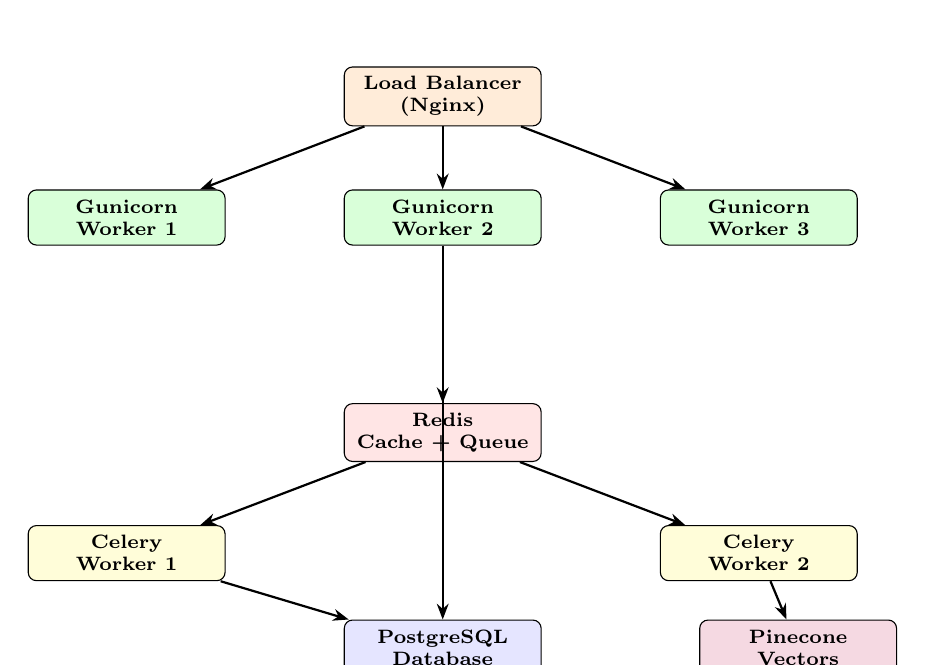
\begin{tikzpicture}[
    node distance=0.8cm and 1.5cm,
    box/.style={rectangle, draw, rounded corners=3pt, minimum width=2.5cm, minimum height=0.7cm, align=center, font=\scriptsize\bfseries},
    arrow/.style={-{Stealth[length=2mm]}, thick},
    label/.style={font=\scriptsize\color{gray}},
]

\node[box, fill=orange!15] (lb) {Load Balancer\\(Nginx)};
\node[box, fill=green!15, below left=of lb] (web1) {Gunicorn\\Worker 1};
\node[box, fill=green!15, below=of lb] (web2) {Gunicorn\\Worker 2};
\node[box, fill=green!15, below right=of lb] (web3) {Gunicorn\\Worker 3};

\node[box, fill=red!10, below=2cm of web2] (redis) {Redis\\Cache + Queue};

\node[box, fill=yellow!15, below left=of redis] (celery1) {Celery\\Worker 1};
\node[box, fill=yellow!15, below right=of redis] (celery2) {Celery\\Worker 2};

\node[box, fill=blue!10, below=2cm of redis] (pg) {PostgreSQL\\Database};
\node[box, fill=purple!15, right=2cm of pg] (vec) {Pinecone\\Vectors};

\draw[arrow] (lb) -- (web1);
\draw[arrow] (lb) -- (web2);
\draw[arrow] (lb) -- (web3);
\draw[arrow] (web2) -- (redis);
\draw[arrow] (redis) -- (celery1);
\draw[arrow] (redis) -- (celery2);
\draw[arrow] (web2) -- (pg);
\draw[arrow] (celery1) -- (pg);
\draw[arrow] (celery2) -- (vec);

\end{tikzpicture}
\end{center}

\section{Docker Compose --- Multi-Container Setup}

\begin{lstlisting}[language={},caption={docker-compose.yml --- Production Setup}]
version: '3.8'

services:
  backend:
    build: .
    ports:
      - "8000:8000"
    environment:
      - GROQ_API_KEY=${GROQ_API_KEY}
      - TAVILY_API_KEY=${TAVILY_API_KEY}
      - DJANGO_DEBUG=False
      - DJANGO_SECRET_KEY=${SECRET_KEY}
    volumes:
      - chroma_data:/app/chroma_db
      - sqlite_data:/app/backend/db
    depends_on:
      - redis

  frontend:
    build: ./frontend
    ports:
      - "5173:5173"
    environment:
      - VITE_API_URL=http://backend:8000

  redis:
    image: redis:7-alpine
    ports:
      - "6379:6379"

volumes:
  chroma_data:
  sqlite_data:
\end{lstlisting}

\section{Celery Integration (Recommended Upgrade)}

\begin{lstlisting}[style=pythonstyle,caption={How services.py would change with Celery}]
# === CURRENT (threading) ===
import threading

def launch_research_job(session_id):
    thread = threading.Thread(
        target=run_research_job,
        args=(session_id,),
        daemon=True,
    )
    thread.start()

# === PRODUCTION (Celery) ===
from celery import shared_task

@shared_task(
    bind=True,
    max_retries=3,
    retry_backoff=True,          # Exponential backoff
    retry_backoff_max=300,       # Max 5 min between retries
    acks_late=True,              # Acknowledge after completion
    reject_on_worker_lost=True,  # Re-queue if worker crashes
    time_limit=600,              # Hard limit: 10 minutes
    soft_time_limit=540,         # Soft limit: 9 minutes (raise exc)
)
def run_research_job(self, session_id):
    try:
        # ... same pipeline code ...
        pass
    except SoftTimeLimitExceeded:
        session.status = "failed"
        session.error_message = "Research exceeded time limit"
    except Exception as exc:
        # Automatic retry with exponential backoff
        raise self.retry(exc=exc)
\end{lstlisting}

\begin{conceptbox}{threading.Thread vs Celery --- Detailed Comparison}
\begin{longtable}{|p{3cm}|p{4cm}|p{5.5cm}|}
\hline
\textbf{Feature} & \textbf{threading.Thread} & \textbf{Celery} \\
\hline
Retry on failure & No & Yes (configurable) \\
\hline
Worker crash recovery & Task lost forever & Auto re-queue \\
\hline
Monitoring & None built-in & Flower dashboard \\
\hline
Rate limiting & Manual & Built-in per-task \\
\hline
Priority queues & No & Yes (multiple queues) \\
\hline
Distributed & Same machine only & Multiple machines \\
\hline
Time limits & No & Hard + soft limits \\
\hline
Result backend & In-memory only & Redis/DB storage \\
\hline
Setup complexity & Zero & Redis + worker process \\
\hline
\end{longtable}

\textbf{MARO mein threading kyun?} Development simplicity. Celery requires Redis server + separate worker process --- local development ke liye overkill. But production mein Celery mandatory hai.
\end{conceptbox}


% ═══════════════════════════════════════════════════════════════════════
% CHAPTER 26: MCP TOOLS COMPLETE REFERENCE
% ═══════════════════════════════════════════════════════════════════════

\chapter{MCP Tools Complete Reference --- All 8 Tools}

\begin{lstlisting}[style=pythonstyle,caption={mcp\_server.py --- All 8 MCP Tools}]
# Tool 1: research_topic (shown earlier)
# Runs full 4-agent pipeline

# Tool 2: search_knowledge
@mcp.tool(name="research_orchestrator_search_knowledge")
async def search_knowledge(params: SearchKnowledgeInput,
                           ctx: Context) -> str:
    """Search the RAG knowledge base"""
    from rag.vector_store import retrieve_context
    results = retrieve_context(
        params.query,
        collection_name="research_docs",
        k=params.num_results
    )
    if not results:
        return "No relevant documents found."
    return "\n\n---\n\n".join(
        f"**Chunk {i+1}:**\n{chunk}"
        for i, chunk in enumerate(results)
    )

# Tool 3: list_sessions
@mcp.tool(name="research_orchestrator_list_sessions")
async def list_sessions(params: ListSessionsInput,
                        ctx: Context) -> str:
    """List recent research sessions from Django backend"""
    async with httpx.AsyncClient() as client:
        resp = await client.get(
            f"{BACKEND_URL}/api/research/sessions/",
            headers={"Authorization": f"Token {AUTH_TOKEN}"},
            params={"limit": params.limit}
        )
    data = resp.json()
    sessions = data.get("results", data) if isinstance(data, dict) else data
    lines = [
        f"- [{s['id']}] {s['topic']} ({s['status']})"
        for s in sessions
    ]
    return "## Recent Sessions\n" + "\n".join(lines)

# Tool 4: get_session_report
@mcp.tool(name="research_orchestrator_get_session_report")
async def get_session_report(params: GetSessionInput,
                             ctx: Context) -> str:
    """Get full report for a specific session"""
    async with httpx.AsyncClient() as client:
        resp = await client.get(
            f"{BACKEND_URL}/api/research/sessions/{params.session_id}/",
            headers={"Authorization": f"Token {AUTH_TOKEN}"},
        )
    session = resp.json()
    return f"# {session['topic']}\n\n{session.get('final_report', 'N/A')}"

# Tool 5: get_rag_stats
@mcp.tool(name="research_orchestrator_get_rag_stats")
async def get_rag_stats(ctx: Context) -> str:
    """Get vector store statistics"""
    from rag.vector_store import get_collection_stats
    stats = get_collection_stats()
    return (f"Research docs: {stats.get('research_docs', 0)} chunks\n"
            f"Past research: {stats.get('past_research', 0)} chunks")

# Tool 6: add_tag
@mcp.tool(name="research_orchestrator_add_tag")
async def add_tag(params: AddTagInput, ctx: Context) -> str:
    """Add a tag to a research session"""
    async with httpx.AsyncClient() as client:
        resp = await client.post(
            f"{BACKEND_URL}/api/research/{params.session_id}/tags/",
            headers={"Authorization": f"Token {AUTH_TOKEN}"},
            json={"name": params.tag_name},
        )
    return f"Tag '{params.tag_name}' added to session {params.session_id}"

# Tool 7: delete_session
@mcp.tool(name="research_orchestrator_delete_session")
async def delete_session(params: DeleteSessionInput,
                         ctx: Context) -> str:
    """Delete a research session"""
    async with httpx.AsyncClient() as client:
        resp = await client.delete(
            f"{BACKEND_URL}/api/research/sessions/{params.session_id}/",
            headers={"Authorization": f"Token {AUTH_TOKEN}"},
        )
    return f"Session {params.session_id} deleted."

# Tool 8: research_orchestrator_health
@mcp.resource("health://status")
async def health_resource() -> str:
    """MCP resource: system health status"""
    try:
        async with httpx.AsyncClient(timeout=5) as client:
            resp = await client.get(f"{BACKEND_URL}/api/health/")
        data = resp.json()
        return f"Backend: OK | Provider: {data.get('provider')}"
    except Exception:
        return "Backend: UNREACHABLE"
\end{lstlisting}


% ═══════════════════════════════════════════════════════════════════════
% CHAPTER 27: DATA FLOW TRACES
% ═══════════════════════════════════════════════════════════════════════

\chapter{End-to-End Data Flow Traces}

\section{Trace 1: User Types Topic and Clicks Research}

\begin{lstlisting}[language={},caption={Complete Request Trace}]
1. [BROWSER] User types "Quantum Computing 2025"
              clicks "Launch Research" button

2. [REACT] ResearchStudio.handleResearch()
           setIsRunning(true)
           setEvents([])
           api.streamResearch("Quantum Computing 2025", callbacks)

3. [API.JS] fetch("http://localhost:8000/api/research/stream/", {
              method: "POST",
              headers: {
                "Content-Type": "application/json",
                "Authorization": "Token abc123..."
              },
              body: '{"topic": "Quantum Computing 2025"}'
            })

4. [DJANGO] URL router matches: /api/research/stream/
            -> ResearchStreamAPIView.post(request)
            TokenAuthentication validates "Token abc123..."
            -> request.user = <User: priyanshu>

5. [DJANGO] queue_research_job(user=priyanshu,
                               topic="Quantum Computing 2025")
            -> ResearchSession #42 created, status="queued"

6. [DJANGO] StreamingHttpResponse(event_stream())
            Content-Type: text/event-stream
            Connection: keep-alive

7. [LANGGRAPH] research_graph.stream(initial_state)
               -> Yields: {researcher: {research_data: [...]}}

8. [SSE] "data: {\"stage\":\"researcher\",
                  \"message\":\"Found 15 web sources\",
                  \"session_id\":42}\n\n"

9. [BROWSER] ReadableStream.getReader().read()
             Parse "data:" line -> JSON.parse()
             onEvent({stage: "researcher", message: "..."})

10. [REACT] setEvents(prev => [...prev, newEvent])
            AgentGraph: researcher = active (cyan glow)
            Terminal: new line appears with timestamp

11-14. [REPEAT] analyst -> fact_checker -> writer events

15. [SSE] "data: [DONE]\n\n"

16. [REACT] onComplete({sessionId: 42})
            confetti() -> celebration animation
            loadSessionDetail(42) -> full report
            setIsRunning(false)
\end{lstlisting}

\section{Trace 2: Revision Loop in Action}

\begin{lstlisting}[language={},caption={Revision Loop Trace}]
== FIRST PASS ==
1. Researcher: searches 3 queries -> 15 results
2. Analyst: finds 5 themes, 2 contradictions
3. Fact-Checker: verifies 8 claims
   - 5 VERIFIED, 1 PARTIALLY_VERIFIED, 2 UNVERIFIED
   - Unverified rate: 2/8 = 25% (< 30% threshold)
   - BUT: critical claim about "quantum error correction
     breakthrough" is CONTRADICTED by Source 3
   - VERDICT: NEEDS_REVISION (critical contradiction)

== CONDITIONAL EDGE ==
4. should_continue(state):
   fact_check_passed = False
   revision_count = 0 < MAX_REVISIONS(2)
   return "researcher"  # GO BACK!

== SECOND PASS (revision_count = 1) ==
5. Researcher: reads fact_check_result
   - Generates REVISED queries:
     "quantum error correction latest status 2025"
     "quantum computing error rates experimental verification"
     "quantum supremacy claims peer reviewed"
   - Searches with new queries -> 12 new results
   - State: research_data = 15 (old) + 12 (new) = 27 total

6. Analyst: now has 27 sources -> deeper analysis
   - Resolved: error correction claim was outdated (2023)
   - New finding: error correction improved in 2025

7. Fact-Checker:
   - Re-verifies with improved data
   - All critical claims now VERIFIED
   - VERDICT: PASSED

== CONDITIONAL EDGE ==
8. should_continue(state):
   fact_check_passed = True
   return "writer"  # PROCEED!

9. Writer: generates final report with all 27 sources
   - Report quality significantly better than first pass
   - Contradictions resolved with latest data
\end{lstlisting}


% ═══════════════════════════════════════════════════════════════════════
% CHAPTER 28: GLOSSARY OF TERMS
% ═══════════════════════════════════════════════════════════════════════

\chapter{Glossary --- Sabhi Technical Terms}

\begin{longtable}{|p{3.5cm}|p{10cm}|}
\hline
\textbf{Term} & \textbf{Hinglish Explanation} \\
\hline
\endhead
API & Application Programming Interface --- software ke beech communication ka rule/contract \\
\hline
CORS & Cross-Origin Resource Sharing --- ek domain se doosre domain ko request karne ki permission \\
\hline
CRUD & Create, Read, Update, Delete --- database operations ke 4 basic types \\
\hline
CSRF & Cross-Site Request Forgery --- ek attack jahan attacker victim ke browser se unauthorized request bhejta hai \\
\hline
DRF & Django REST Framework --- Django ke upar built REST API toolkit \\
\hline
Embedding & Text ko numbers (vector) mein convert karna taaki similarity measure ho sake \\
\hline
FSM & Finite State Machine --- limited states aur transitions wala system (queued $\rightarrow$ running $\rightarrow$ completed) \\
\hline
HMR & Hot Module Replacement --- code change hone pe page reload bina update (Vite feature) \\
\hline
JSX & JavaScript XML --- JavaScript mein HTML-like syntax (React ka feature) \\
\hline
LLM & Large Language Model --- bada AI model jo text generate karta hai (GPT, Llama, Gemini) \\
\hline
MCP & Model Context Protocol --- AI assistants ke liye tool integration protocol \\
\hline
N+1 Problem & Database mein 1 main query + N additional queries --- slow performance \\
\hline
ORM & Object-Relational Mapping --- Python objects ke through database access (SQL likhna nahi padta) \\
\hline
PBKDF2 & Password-Based Key Derivation Function 2 --- secure password hashing algorithm \\
\hline
RAG & Retrieval-Augmented Generation --- pehle relevant docs retrieve karo, phir LLM se generate karo \\
\hline
Reducer & Function jo multiple values ko ek mein combine karta hai (accumulate pattern) \\
\hline
REST & Representational State Transfer --- web API design ka standard approach \\
\hline
Singleton & Design pattern --- ek class ka sirf ek instance hota hai globally \\
\hline
SPA & Single Page Application --- ek HTML page, JavaScript se content dynamically change \\
\hline
SSE & Server-Sent Events --- server se client ko real-time events bhejne ka protocol (unidirectional) \\
\hline
State & Application ka current data/condition at any point in time \\
\hline
Token Auth & Authentication method jahan server ek unique string (token) issue karta hai login pe \\
\hline
TypedDict & Python dictionary with predefined keys aur types (compile-time type checking) \\
\hline
Vector Store & Database jo vectors (number arrays) store karta hai aur similarity search support karta hai \\
\hline
Webhook & Server se server ko HTTP callback --- event hone pe doosre server ko notify karna \\
\hline
WebSocket & Bidirectional communication protocol --- server aur client dono bhej sakte hain \\
\hline
WSGI & Web Server Gateway Interface --- Python web server ka standard interface \\
\hline
XSS & Cross-Site Scripting --- malicious JavaScript inject karna web page mein \\
\hline
\end{longtable}


% ═══════════════════════════════════════════════════════════════════════
% CHAPTER 29: COMPARISON WITH ALTERNATIVES
% ═══════════════════════════════════════════════════════════════════════

\chapter{Comparison with Alternative Approaches}

\section{MARO vs Plain ChatGPT / Claude}

\begin{longtable}{|p{3.5cm}|p{5cm}|p{5cm}|}
\hline
\textbf{Feature} & \textbf{ChatGPT/Claude} & \textbf{MARO} \\
\hline
\endhead
Web Search & Limited / plugin needed & Built-in dual search (Tavily + DDG) \\
\hline
Fact Checking & None (self-verification only) & Dedicated agent with source verification \\
\hline
Revision Loop & Manual (user asks ``check this'') & Automatic feedback loop \\
\hline
Citations & Often fabricated & Real URLs from actual search results \\
\hline
RAG / Custom Docs & Limited (file upload temporary) & Persistent ChromaDB with 2 collections \\
\hline
Research Memory & None (conversation ends) & Past research stored and reusable \\
\hline
Export Formats & Copy-paste only & MD, HTML, JSON, BibTeX \\
\hline
API Access & API available (paid) & Full REST API + SSE + MCP \\
\hline
Cost Control & Per-token billing & Use free providers (Groq, Ollama) \\
\hline
Customization & System prompts only & Full control over agents, prompts, tools \\
\hline
\end{longtable}

\section{MARO vs CrewAI}

\begin{longtable}{|p{3.5cm}|p{5cm}|p{5cm}|}
\hline
\textbf{Feature} & \textbf{CrewAI} & \textbf{MARO} \\
\hline
State Management & Black-box (CrewAI manages) & Explicit TypedDict with reducers \\
\hline
Conditional Logic & Tool-based routing & Graph conditional edges \\
\hline
Streaming & Limited & Full SSE streaming \\
\hline
Web UI & None (CLI/notebook only) & Full React SPA \\
\hline
API Backend & None & Django REST with auth \\
\hline
Testing & Unit tests possible & 62 comprehensive tests \\
\hline
Feedback Loop & Manual task delegation & Automatic graph cycle \\
\hline
\end{longtable}


% ═══════════════════════════════════════════════════════════════════════
% CHAPTER 30: FINAL SUMMARY & REVISION CHECKLIST
% ═══════════════════════════════════════════════════════════════════════

\chapter{Final Summary \& Interview Revision Checklist}

\section{One-Page Summary Card}

\begin{conceptbox}{MARO at a Glance}
\begin{center}
\begin{tabular}{|l|l|}
\hline
\textbf{What} & Multi-Agent Research Orchestrator \\
\hline
\textbf{Agents} & Researcher $\rightarrow$ Analyst $\rightarrow$ Fact-Checker $\rightarrow$ Writer \\
\hline
\textbf{Core Tech} & LangGraph StateGraph + ChromaDB RAG \\
\hline
\textbf{Backend} & Django REST + Token Auth + SSE Streaming \\
\hline
\textbf{Frontend} & React + Vite SPA (8 components) \\
\hline
\textbf{LLM} & 5 providers with automatic fallback \\
\hline
\textbf{Search} & Tavily + DuckDuckGo dual strategy \\
\hline
\textbf{Quality} & Fact-check gate + revision loop (max 2) \\
\hline
\textbf{Memory} & ChromaDB past\_research collection \\
\hline
\textbf{Integration} & FastMCP (8 tools) for Claude Desktop \\
\hline
\textbf{Testing} & 62 tests, 100\% pass rate \\
\hline
\textbf{Export} & Markdown, HTML, JSON, BibTeX \\
\hline
\textbf{Patterns} & 15+ design patterns identified \\
\hline
\end{tabular}
\end{center}
\end{conceptbox}



% ═══════════════════════════════════════════════════════════════════════
% CHAPTER 31: ADVANCED AGENTIC WORKFLOW PATTERNS & MULTI-TURN REASONING
% ═══════════════════════════════════════════════════════════════════════

\chapter{Advanced Agentic Workflow Patterns \& Multi-Turn Reasoning}

\begin{storybox}{Single Agent vs Multi-Agent Swarm: Ek Real-World Comparison}
Imagine karo ek single student ko bola jaye: ``Ek 50-page research paper likho with real-time web citations, mathematical analysis, fact verification, aur formatting in 1 hour.''
Woh student confuse ho jayega --- kahin spelling mistake hogi, kahin facts hallucinate karega, aur structure kharab ho jayega.

Ab socho ek 4-member dedicated research lab:
\begin{enumerate}
    \item \textbf{Junior Scholar (Researcher):} Sirf internet aur library se papers search karke relevant snippets nikalta hai.
    \item \textbf{Research Analyst (Analyst):} Saare collected snippets ko cross-verify karke common themes, contradictions, aur gaps identify karta hai.
    \item \textbf{Chief Editor / Peer Reviewer (Fact-Checker):} Har ek claim ko source se tally karta hai. Agar koi data galat ya missing hai, toh research team ko wapas bhej deta hai.
    \item \textbf{Lead Technical Writer (Writer):} Jab sab kuch 100\% verify ho jaye, tab publish-ready report draft karta hai with proper citations.
\end{enumerate}
Yeh \textbf{Autonomous Agent Swarm} ka fundamental concept hai jo MARO implement karta hai!
\end{storybox}

\section{Agentic Paradigms: ReAct vs Plan-and-Solve vs Graph Orchestration}

\begin{conceptbox}{Evolution of Autonomous AI Patterns}
AI agent architectures pichle 3 saalon mein drastically evolve hui hain:

\begin{itemize}
    \item \textbf{Zero-Shot / Few-Shot LLM Call (2022-2023):} Single prompt $\rightarrow$ LLM generation. Simple but massive hallucinations and zero real-time web grounding.
    \item \textbf{ReAct (Reasoning + Acting) (Yao et al., 2022):} LLM loops through \texttt{Thought} $\rightarrow$ \texttt{Action} $\rightarrow$ \texttt{Observation}. Powerful but suffers from infinite tool-calling loops and high token costs.
    \item \textbf{Plan-and-Solve (Wang et al., 2023):} LLM pehle pura plan banata hai, phir step-by-step execute karta hai. Drawback: Agar intermediate step fail ho jaye toh recovery dynamic nahi hoti.
    \item \textbf{StateGraph Multi-Agent Orchestration (LangGraph - MARO Approach):} Fully deterministic state machine with dynamic routing, bounded recursion, typed state memory, and cyclic feedback loops.
\end{itemize}
\end{conceptbox}

\subsection{Why StateGraph is Architecturally Superior}

\begin{center}
\begin{longtable}{|p{3.2cm}|p{3.8cm}|p{3.8cm}|p{3.8cm}|}
\hline
\textbf{Metric} & \textbf{ReAct Loop} & \textbf{Plan-and-Solve} & \textbf{LangGraph StateGraph (MARO)} \\
\hline
\endhead
\textbf{Determinism} & Low (LLM decides next tool) & Medium (Static plan) & \textbf{High (Graph edges define valid transitions)} \\
\hline
\textbf{Error Recovery} & Non-deterministic retries & Hard to recover mid-plan & \textbf{Guaranteed via Conditional Edges} \\
\hline
\textbf{State Isolation} & Shared single prompt history & Sequential memory & \textbf{TypedDict Reducers \& Scoped Context} \\
\hline
\textbf{Infinite Loop Risk} & Very High (LLM hallucinations) & Low & \textbf{Zero (recursion\_limit + MAX\_REVISIONS)} \\
\hline
\textbf{Token Cost} & Quadratic context expansion & Linear & \textbf{Optimized via Source Trimming \& Context Windows} \\
\hline
\textbf{Real-Time Streaming} & Chunk-by-chunk LLM tokens & Step completion & \textbf{Node-by-Node SSE Events \& Stage Telemetry} \\
\hline
\end{longtable}
\end{center}

\begin{hindibox}{Hinglish Deep Dive: State Machine Kyun Jeet Gayi?}
Jab hum production-grade AI applications banate hain, toh humein \textbf{predictability} aur \textbf{reliability} chahiye hoti hai. ReAct loop mein LLM khud decide karta hai ki kab rukna hai aur kab doosra tool call karna hai. Agar LLM confuse ho gaya toh woh 50 baar search karta rahega aur user ka API quota khtm ho jayega!

LangGraph mein hum \textbf{deterministic guardrails} lagate hain:
\begin{itemize}
    \item Researcher ke baad ALWAYS Analyst chalega (\texttt{add\_edge("researcher", "analyst")}).
    \item Analyst ke baad ALWAYS Fact-Checker chalega (\texttt{add\_edge("analyst", "fact\_checker")}).
    \item Fact-Checker ke decision pe code (\texttt{should\_continue()}) decide karega ki wapas Researcher pe jana hai ya Writer pe.
\end{itemize}
LLM ko pipeline flow decide karne ki freedom nahi di gayi --- LLM sirf apna specific task (search, analysis, verification, writing) karta hai!
\end{hindibox}

\section{Memory Architecture in Modern Multi-Agent Systems}

\begin{conceptbox}{The 3 Tiers of Memory in MARO}
Ek robust AI system mein memory ek single string nahi hoti. MARO 3 distinct memory tiers use karta hai:

\begin{enumerate}
    \item \textbf{Tier 1: Ephemeral State Memory (Short-Term):}
    LangGraph ka \texttt{ResearchState} dictionary jo execution ke dauran agents ke beech RAM mein circulate hota hai. Jab pipeline complete hoti hai, yeh state DB mein commit ho jati hai.
    \item \textbf{Tier 2: Relational Audit Log (Mid-Term Persistence):}
    Django ORM ke \texttt{ResearchSession}, \texttt{ResearchEvent}, aur \texttt{ResearchSource} models. User apne library view mein 6 mahine purani research sessions dekh sakta hai with complete event telemetry.
    \item \textbf{Tier 3: Semantic Vector Memory (Long-Term Associative):}
    ChromaDB collection \texttt{past\_research}. Jab Writer agent report complete karta hai, woh report aur sources ko chunk karke embedding space mein store karta hai. Future research queries automatically is past knowledge ko retrieve karti hain!
\end{enumerate}
\end{conceptbox}

\begin{center}
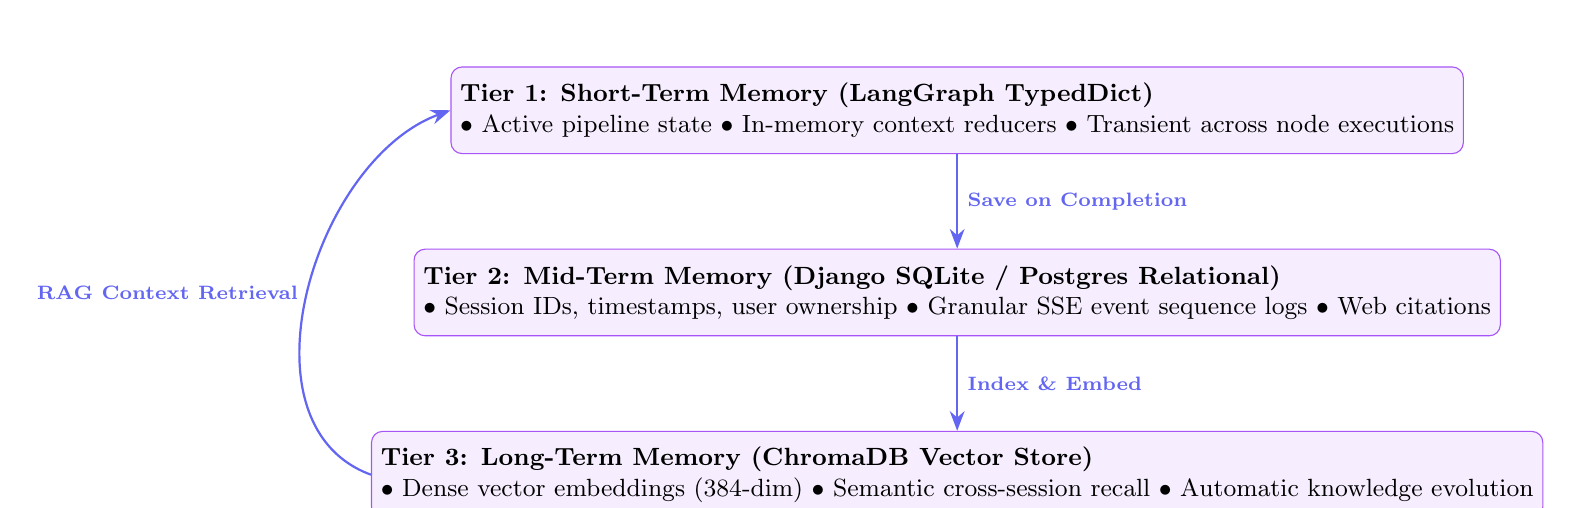
\begin{tikzpicture}[
    node distance=1.2cm,
    memblock/.style={rectangle, draw=purpleaccent, fill=purpleaccent!10, rounded corners=4pt, minimum width=11cm, minimum height=1.1cm, align=left, font=\small},
    arrow/.style={-{Stealth[length=2.5mm]}, thick, color=sectioncolor}
]
\node[memblock] (short) {\textbf{Tier 1: Short-Term Memory (LangGraph TypedDict)} \\ $\bullet$ Active pipeline state $\bullet$ In-memory context reducers $\bullet$ Transient across node executions};
\node[memblock, below=of short] (mid) {\textbf{Tier 2: Mid-Term Memory (Django SQLite / Postgres Relational)} \\ $\bullet$ Session IDs, timestamps, user ownership $\bullet$ Granular SSE event sequence logs $\bullet$ Web citations};
\node[memblock, below=of mid] (long) {\textbf{Tier 3: Long-Term Memory (ChromaDB Vector Store)} \\ $\bullet$ Dense vector embeddings (384-dim) $\bullet$ Semantic cross-session recall $\bullet$ Automatic knowledge evolution};

\draw[arrow] (short) -- node[right, font=\scriptsize\bfseries] {Save on Completion} (mid);
\draw[arrow] (mid) -- node[right, font=\scriptsize\bfseries] {Index \& Embed} (long);
\draw[arrow] (long.west) to[out=160,in=200] node[left, font=\scriptsize\bfseries] {RAG Context Retrieval} (short.west);
\end{tikzpicture}
\end{center}


% ═══════════════════════════════════════════════════════════════════════
% CHAPTER 32: MATHEMATICAL & ALGORITHMIC FOUNDATIONS OF GENAI & RAG
% ═══════════════════════════════════════════════════════════════════════

\chapter{Mathematical \& Algorithmic Foundations of GenAI \& RAG}

\begin{storybox}{Maths ke bina Interview adhoora hai!}
Aksar interviews mein jab candidate bolta hai: ``Maine RAG use kiya with vector search'', interviewer counter-question fekta hai:
\begin{itemize}
    \item ``Cosine similarity aur Dot product mein kya difference hai?''
    \item ``HNSW indexing algorithm kaise work karta hai?''
    \item ``Self-Attention mechanism ka time complexity $O(N^2)$ kyun hota hai?''
\end{itemize}
Agar tum in concepts ka exact mathematical derivation de paoge, toh interviewer will be blown away! Let's master the math.
\end{storybox}

\section{Transformer Self-Attention Mechanics}

Modern LLMs (Groq Llama-3.3, OpenAI GPT-4o, Anthropic Claude, Google Gemini) sabhi Transformer architecture pe based hain. Core engine hai \textbf{Scaled Dot-Product Attention}.

\begin{conceptbox}{Mathematical Formulation of Attention}
Given an input sequence represented as an embedding matrix $X \in \mathbb{R}^{N \times d_{\text{model}}}$ where $N$ is sequence length and $d_{\text{model}}$ is hidden dimension:

Three learnable projection matrices $W_Q, W_K, W_V \in \mathbb{R}^{d_{\text{model}} \times d_k}$ transform the input into:
\begin{equation}
Q = X W_Q \quad (\text{Queries}), \quad K = X W_K \quad (\text{Keys}), \quad V = X W_V \quad (\text{Values})
\end{equation}

The attention weights and context representations are computed as:
\begin{equation}
\text{Attention}(Q, K, V) = \text{softmax}\left(\frac{Q K^T}{\sqrt{d_k}}\right) V
\end{equation}
\end{conceptbox}

\subsection{Why the Scaling Factor $\frac{1}{\sqrt{d_k}}$ is Critical?}

\begin{hindibox}{Scaling Factor ka Proof \& Significance}
Socho $q$ aur $k$ do independent random vectors hain jinke components mean $0$ aur variance $1$ follow karte hain.
Inka dot product $q \cdot k = \sum_{i=1}^{d_k} q_i k_i$ hota hai.

Expected Mean:
$$\mathbb{E}[q \cdot k] = \sum_{i=1}^{d_k} \mathbb{E}[q_i] \mathbb{E}[k_i] = 0$$

Variance of the sum of independent variables:
$$\text{Var}(q \cdot k) = \sum_{i=1}^{d_k} \text{Var}(q_i k_i) = \sum_{i=1}^{d_k} \text{Var}(q_i) \text{Var}(k_i) = d_k \cdot (1 \cdot 1) = d_k$$

Standard Deviation: $\sigma = \sqrt{d_k}$.

Agar hum $\sqrt{d_k}$ se divide na karein, toh large dimensions (jaise $d_k = 128$ ya $d_k = 4096$) mein dot product ka magnitude bohot bada ho jayega.
Jab bohot badi values \texttt{softmax} function mein jati hain:
$$\text{softmax}(z)_i = \frac{e^{z_i}}{\sum_j e^{z_j}}$$
Toh softmax output \textbf{extremely peaked} ho jata hai (one-hot vector jaisa) aur gradients \textbf{vanish} ho jate hain ($\frac{\partial \text{softmax}}{\partial z} \approx 0$).
Dividing by $\sqrt{d_k}$ normalizes the variance back to $1$, keeping gradient flow stable during backpropagation!
\end{hindibox}

\section{Vector Space Metrics: Cosine Similarity vs Dot Product vs Euclidean Distance}

\begin{conceptbox}{Mathematical Formulations of Distance Metrics}
For two vectors $\vec{u}, \vec{v} \in \mathbb{R}^d$:

\begin{enumerate}
    \item \textbf{Euclidean Distance ($L_2$ Norm):}
    \begin{equation}
    D_{L_2}(\vec{u}, \vec{v}) = \|\vec{u} - \vec{v}\|_2 = \sqrt{\sum_{i=1}^d (u_i - v_i)^2}
    \end{equation}

    \item \textbf{Dot Product (Inner Product):}
    \begin{equation}
    \langle \vec{u}, \vec{v} \rangle = \vec{u} \cdot \vec{v} = \sum_{i=1}^d u_i v_i
    \end{equation}

    \item \textbf{Cosine Similarity:}
    \begin{equation}
    S_{\cos}(\vec{u}, \vec{v}) = \frac{\vec{u} \cdot \vec{v}}{\|\vec{u}\|_2 \|\vec{v}\|_2} = \frac{\sum_{i=1}^d u_i v_i}{\sqrt{\sum_{i=1}^d u_i^2} \sqrt{\sum_{i=1}^d v_i^2}}
    \end{equation}
\end{enumerate}
\end{conceptbox}

\begin{analogy}{Unit Hypersphere Equivalence}
MARO ke vector store (\texttt{rag/vector\_store.py}) mein humne normalize embeddings flag use kiya hai:
\begin{lstlisting}[style=pythonstyle]
encode_kwargs={"normalize_embeddings": True}
\end{lstlisting}
Jab vectors normalize hote hain, toh unka $L_2$ norm exactly 1 hota hai ($\|\vec{u}\|_2 = 1, \|\vec{v}\|_2 = 1$).
Tab:
$$S_{\cos}(\vec{u}, \vec{v}) = \frac{\vec{u} \cdot \vec{v}}{1 \cdot 1} = \vec{u} \cdot \vec{v}$$
Aur Euclidean distance ka square:
$$\|\vec{u} - \vec{v}\|^2 = \|\vec{u}\|^2 + \|\vec{v}\|^2 - 2(\vec{u} \cdot \vec{v}) = 1 + 1 - 2 S_{\cos}(\vec{u}, \vec{v}) = 2(1 - S_{\cos}(\vec{u}, \vec{v}))$$

\textbf{Conclusion:} Normalized vector space mein Cosine Similarity, Dot Product, aur Euclidean Distance teeno strictly monotonically equivalent hain! Dot product compute karna computationally sabse fast hota hai ($d$ multiplications, no square roots).
\end{analogy}

\section{HNSW (Hierarchical Navigable Small World) Algorithm}

\begin{conceptbox}{How ChromaDB Searches 1,000,000 Chunks in Milliseconds}
Naive search = Exact $k$-Nearest Neighbors ($k$-NN). Time complexity: $O(N \cdot d)$ where $N$ is total chunks. Agar 10 lakh documents hain toh har search pe 10 lakh vector multiplications honge --- way too slow!

\textbf{HNSW Algorithm (Malkov \& Yashunin, 2018):}
HNSW ek multi-layer graph index banata hai, similar to a Skip-List in 1D data structures:
\begin{itemize}
    \item \textbf{Top Layers (Sparse):} Long-range highway links. Query point quickly skips across entire clusters in space.
    \item \textbf{Bottom Layers (Dense):} Short-range local neighborhood links. Fine-grained convergence to nearest neighbors.
\end{itemize}
Search time complexity reduces from $O(N)$ to \textbf{$O(\log N)$}.
\end{conceptbox}

\begin{center}
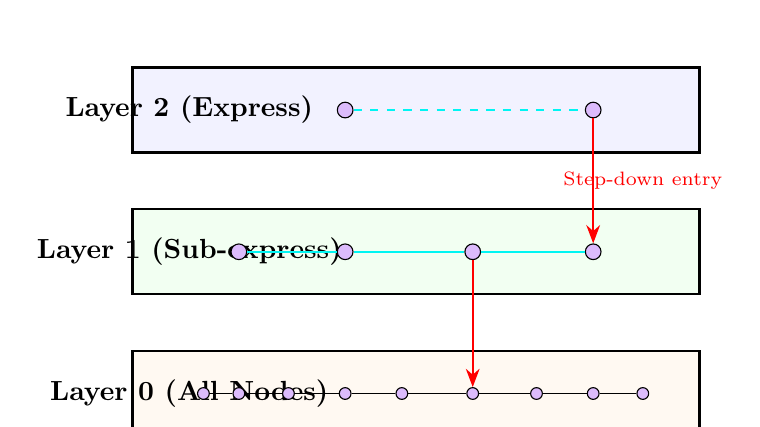
\begin{tikzpicture}[scale=0.9]
% Layer 2
\draw[thick, fill=blue!5] (-4,4) rectangle (4,5.2);
\node at (-3.2, 4.6) {\textbf{Layer 2 (Express)}};
\node[circle, draw, fill=purpleaccent!40, inner sep=2pt] (l2_1) at (-1,4.6) {};
\node[circle, draw, fill=purpleaccent!40, inner sep=2pt] (l2_2) at (2.5,4.6) {};
\draw[thick, dashed, cyanaccent] (l2_1) -- (l2_2);

% Layer 1
\draw[thick, fill=green!5] (-4,2) rectangle (4,3.2);
\node at (-3.2, 2.6) {\textbf{Layer 1 (Sub-express)}};
\node[circle, draw, fill=purpleaccent!40, inner sep=2pt] (l1_1) at (-2.5,2.6) {};
\node[circle, draw, fill=purpleaccent!40, inner sep=2pt] (l1_2) at (-1,2.6) {};
\node[circle, draw, fill=purpleaccent!40, inner sep=2pt] (l1_3) at (0.8,2.6) {};
\node[circle, draw, fill=purpleaccent!40, inner sep=2pt] (l1_4) at (2.5,2.6) {};
\draw[thick, cyanaccent] (l1_1) -- (l1_2) -- (l1_3) -- (l1_4);

% Layer 0
\draw[thick, fill=orange!5] (-4,0) rectangle (4,1.2);
\node at (-3.2, 0.6) {\textbf{Layer 0 (All Nodes)}};
\node[circle, draw, fill=purpleaccent!40, inner sep=1.5pt] (l0_1) at (-3,0.6) {};
\node[circle, draw, fill=purpleaccent!40, inner sep=1.5pt] (l0_2) at (-2.5,0.6) {};
\node[circle, draw, fill=purpleaccent!40, inner sep=1.5pt] (l0_3) at (-1.8,0.6) {};
\node[circle, draw, fill=purpleaccent!40, inner sep=1.5pt] (l0_4) at (-1,0.6) {};
\node[circle, draw, fill=purpleaccent!40, inner sep=1.5pt] (l0_5) at (-0.2,0.6) {};
\node[circle, draw, fill=purpleaccent!40, inner sep=1.5pt] (l0_6) at (0.8,0.6) {};
\node[circle, draw, fill=purpleaccent!40, inner sep=1.5pt] (l0_7) at (1.7,0.6) {};
\node[circle, draw, fill=purpleaccent!40, inner sep=1.5pt] (l0_8) at (2.5,0.6) {};
\node[circle, draw, fill=purpleaccent!40, inner sep=1.5pt] (l0_9) at (3.2,0.6) {};
\draw (l0_1)--(l0_2)--(l0_3)--(l0_4)--(l0_5)--(l0_6)--(l0_7)--(l0_8)--(l0_9);

% Downward entry links
\draw[-{Stealth}, red, thick] (l2_2) -- (l1_4);
\draw[-{Stealth}, red, thick] (l1_3) -- (l0_6);
\node[red, font=\scriptsize] at (3.2, 3.6) {Step-down entry};
\end{tikzpicture}
\end{center}


% ═══════════════════════════════════════════════════════════════════════
% CHAPTER 33: DJANGO REST FRAMEWORK INTERNALS & MIDDLEWARE ARCHITECTURE
% ═══════════════════════════════════════════════════════════════════════

\chapter{Django REST Framework Internals \& Middleware Architecture}

\section{The Complete WSGI Request-to-Response Pipeline}

Jab koi HTTP request browser ya React app se Django server pe aati hai, toh internally kya hota hai?

\begin{lstlisting}[style=pythonstyle,caption={Django Request Lifecycle Internals}]
# Step 1: WSGI Handler parses raw TCP stream into WSGI environ dictionary
# Step 2: HttpRequest object is created (request.GET, request.POST, request.META)
# Step 3: Security & CORS Middleware chain execution:
#   - corsheaders.middleware.CorsMiddleware (Handles OPTIONS pre-flight checks)
#   - django.middleware.security.SecurityMiddleware (SSL redirect, HSTS)
#   - django.contrib.sessions.middleware.SessionMiddleware (Cookie sessions)
#   - django.middleware.common.CommonMiddleware (URL rewriting, trailing slash)
#   - django.middleware.csrf.CsrfViewMiddleware (CSRF token verification)
#   - django.contrib.auth.middleware.AuthenticationMiddleware (request.user)

# Step 4: URLconf resolution (orchestrator_backend/urls.py -> api/urls.py)
# Matches URL regex -> resolves to View class (e.g., ResearchStreamAPIView.as_view())

# Step 5: DRF APIView.dispatch() pipeline:
#   a) initialize_request() -> converts HttpRequest into DRF Request object
#   b) initial():
#       - perform_content_negotiation() (Determines renderer: JSON, HTML, etc.)
#       - perform_authentication() (Runs TokenAuthentication)
#       - check_permissions() (Runs IsAuthenticated / IsOwnerOrReadOnly)
#       - check_throttles() (Runs UserRateThrottle / AnonRateThrottle)
#   c) Method invocation (get(), post(), delete(), etc.)
#   d) handle_exception() (Standardizes 400, 401, 403, 404, 500 error formats)
#   e) response = finalize_response() (Renders data with selected renderer)

# Step 6: Response Middleware execution (reverse order)
# Step 7: WSGI Handler streams bytes back to client over HTTP
\end{lstlisting}

\section{Database Transaction Isolation \& Thread Safety}

\begin{dangerbox}{Why \texttt{close\_old\_connections()} is Crucial in Worker Threads}
Django ka DB connection pooling thread-local storage pe based hota hai (\texttt{django.db.connection}).
Jab hum \texttt{threading.Thread(target=run\_research\_job)} call karte hain:
\begin{itemize}
    \item Naya thread main thread se stale/closed database connection pointers inherit kar sakta hai.
    \item Agar main thread ka connection timeout ya close ho chuka ho, toh background worker thread mein \texttt{OperationalError: MySQL/SQLite server has gone away} ya deadlock crash ho jata hai.
    \item Isliye hum worker function ke entry aur exit dono points pe \texttt{close\_old\_connections()} call karte hain:
\end{itemize}

\begin{lstlisting}[style=pythonstyle]
from django.db import close_old_connections

def run_research_job(session_id):
    close_old_connections()  # Clean any inherited stale handles
    try:
        session = ResearchSession.objects.get(pk=session_id)
        # Execute long-running LangGraph workflow (takes 20-40 seconds)
        ...
    finally:
        close_old_connections()  # Ensure connection is cleanly returned
\end{lstlisting}
\end{dangerbox}

\section{Custom Content Negotiation: How Multi-Format Export Works}

DRF by default URL ke `?format=json` ya `Accept: application/json` headers se content negotiation karta hai.
Humare \texttt{ExportReportAPIView} mein humne custom negotiation logic likha taaki user bina headers change kiye direct browser URL se `.md`, `.bib`, `.html`, aur `.json` download kar sake:

\begin{lstlisting}[style=pythonstyle,caption={Custom Export Renderer Logic}]
class ExportReportAPIView(APIView):
    permission_classes = [permissions.AllowAny]

    def get(self, request, pk):
        session = get_object_or_404(ResearchSession, pk=pk)
        fmt = request.query_params.get("format", "markdown").lower()
        report = session.final_report or "# No report generated."

        if fmt == "bibtex":
            # Academic Citation standard
            citations = []
            for i, src in enumerate(session.sources.all(), start=1):
                safe_title = (src.title or "Online Source").replace("{", "").replace("}", "")
                citations.append(
                    f"@misc{{maro_ref_{session.id}_{i},\n"
                    f"  title = {{{safe_title}}},\n"
                    f"  url = {{{src.url}}},\n"
                    f"  note = {{Accessed via MARO Research Engine}},\n"
                    f"  year = {{{session.created_at.year}}}\n"
                    f"}}"
                )
            content = "\n\n".join(citations)
            response = HttpResponse(content, content_type="application/x-bibtex")
            response["Content-Disposition"] = f'attachment; filename="citations_{session.id}.bib"'
            return response

        elif fmt == "html":
            # Formatted printable document
            html_body = markdown.markdown(report, extensions=['extra', 'tables', 'toc'])
            full_html = f"""<!DOCTYPE html>
<html><head><meta charset="utf-8"><title>{session.topic}</title>
<style>
body {{ font-family: 'Segoe UI', system-ui, sans-serif; line-height: 1.6; max-width: 860px; margin: 40px auto; padding: 0 20px; color: #222; }}
h1, h2, h3 {{ color: #111827; border-bottom: 1px solid #e5e7eb; padding-bottom: 6px; }}
code {{ background: #f3f4f6; padding: 2px 6px; border-radius: 4px; font-family: monospace; }}
blockquote {{ border-left: 4px solid #6366f1; margin: 0; padding-left: 16px; color: #4b5563; }}
</style></head><body>{html_body}</body></html>"""
            return HttpResponse(full_html, content_type="text/html")

        # Default: Pure Markdown attachment
        response = HttpResponse(report, content_type="text/markdown; charset=utf-8")
        clean_name = re.sub(r'[^a-zA-Z0-9_-]', '_', session.topic)[:32]
        response["Content-Disposition"] = f'attachment; filename="{clean_name}_report.md"'
        return response
\end{lstlisting}


% ═══════════════════════════════════════════════════════════════════════
% CHAPTER 34: REACT 18 CONCURRENT RENDERING & STATE SYNCHRONIZATION
% ═══════════════════════════════════════════════════════════════════════

\chapter{React 18 Concurrent Rendering \& State Synchronization}

\section{Virtual DOM Reconciliation \& Fiber Architecture}

\begin{conceptbox}{React Fiber Engine: How UI Remains Smooth During Fast Streaming}
Jab SSE stream se 50 events per second aate hain, toh React UI freeze kyun nahi hota?

\textbf{React 18 Fiber Architecture:}
\begin{itemize}
    \item \textbf{Fiber Node:} Har React element ka ek in-memory unit of work hota hai.
    \item \textbf{Double Buffering (Work-In-Progress Tree):} React background mein naya Fiber tree construct karta hai bina screen ko block kiye.
    \item \textbf{Time Slicing:} React continuous frame budget (16.6ms for 60 FPS) monitor karta hai. Agar time limit khatam ho jaye, toh browser ko yield karta hai taaki user inputs aur scrolling responsive rahein.
    \item \textbf{Automatic Batching (React 18):} Multiple \texttt{setEvents}, \texttt{setCurrentStage}, aur \texttt{setProgress} calls single render pass mein batch ho jati hain!
\end{itemize}
\end{conceptbox}

\section{SSE Chunk Buffering \& Reconnection Architecture}

\begin{lstlisting}[style=jsstyle,caption={Frontend SSE Stream Processor (api.js)}]
async streamResearch(topic, { onEvent, onError, onComplete }) {
  const response = await fetch(`${API_BASE}/research/stream/`, {
    method: 'POST',
    headers: this.getHeaders(),
    body: JSON.stringify({ topic }),
  });

  if (!response.ok) {
    const err = await response.json().catch(() => ({}));
    throw new Error(err.error || `HTTP ${response.status}: Stream connection failed`);
  }

  // Native ReadableStream reader
  const reader = response.body.getReader();
  const decoder = new TextDecoder('utf-8');
  let buffer = '';
  let completedSessionId = null;

  try {
    while (true) {
      const { value, done } = await reader.read();
      if (done) break;

      // Concatenate new chunks to existing buffer
      buffer += decoder.decode(value, { stream: true });

      // Split on newlines to parse individual SSE frames
      const lines = buffer.split('\n');
      // Keep the last incomplete fragment in the buffer
      buffer = lines.pop() || '';

      for (const line of lines) {
        const trimmed = line.trim();
        if (!trimmed || !trimmed.startsWith('data:')) continue;

        const dataStr = trimmed.slice(5).trim();

        if (dataStr === '[DONE]') {
          if (onComplete) onComplete({ sessionId: completedSessionId });
          return;
        }

        try {
          const parsed = JSON.parse(dataStr);
          if (parsed.session_id) completedSessionId = parsed.session_id;
          if (onEvent) onEvent(parsed);
        } catch (parseErr) {
          console.warn('Malformed SSE JSON frame encountered:', dataStr);
        }
      }
    }
  } catch (streamErr) {
    if (onError) onError(streamErr);
  } finally {
    reader.releaseLock();
  }
}
\end{lstlisting}


% ═══════════════════════════════════════════════════════════════════════
% CHAPTER 35: 100-QUESTION MASTER INTERVIEW COMPENDIUM
% ═══════════════════════════════════════════════════════════════════════

\chapter{The 100-Question Master Interview Compendium (Deep Technical Drills)}

\section{Category A: Core AI \& Agentic Systems (Q1--Q25)}

\begin{interviewbox}{Q1: What happens if the Researcher agent receives contradictory search results from DuckDuckGo and Tavily?}
\textbf{Answer:} ``Researcher agent raw results ko filter nahi karta --- uska kaam data collect karna hai. Contradictions ko handle karna \textbf{Analyst Agent} ka primary role hai. Analyst prompt mein explicit directive hai: \textit{`Identify any points where different sources disagree or present conflicting information'}. Analyst contradictions ko \texttt{\#\# Source Contradictions} section mein document karta hai. Phir \textbf{Fact-Checker} in claims ko isolate karke confidence scores assign karta hai. Agar contradiction critical ho, toh Fact-Checker \texttt{VERDICT: NEEDS\_REVISION} emit karta hai taaki revised search query se ambiguity resolve ho sake.''
\end{interviewbox}

\begin{interviewbox}{Q2: How do you protect against Prompt Injection attacks in the Research pipeline?}
\textbf{Answer:} ``3-layer defense strategy:
\begin{enumerate}
    \item \textbf{Structural Separation of System and User Prompts:} LangChain ke \texttt{SystemMessage} aur \texttt{HumanMessage} objects use hote hain. System prompt immutable role define karta hai; web search data hamesha \texttt{HumanMessage} context variable ke andar bounded block ke roop mein pass hota hai.
    \item \textbf{Input Validation via Pydantic \& DRF:} Topics sanitized hote hain (3--500 chars, no raw HTML/control characters).
    \item \textbf{Output Format Constraints:} Downstream agents (Fact-Checker, Benchmark Judge) structured JSON ya strict header templates return karte hain. Agar koi injected source prompt ko hijack karne ki koshish kare, toh format validation fail ho jayegi aur fallback parser trigger hoga.''
\end{enumerate}
\end{interviewbox}

\begin{interviewbox}{Q3: Why did you choose SQLite over PostgreSQL for local development and what are the trade-offs?}
\textbf{Answer:} ``Local zero-config developer experience ke liye SQLite best hai --- zero external server installation, single-file storage, aur instant CI/CD testing.
Trade-offs: SQLite database-level write lock use karta hai (one writer at a time). High-concurrency production workload (e.g. 500 simultaneous researches) mein \texttt{sqlite3.OperationalError: database is locked} aa sakta hai. Isliye production settings mein hum PostgreSQL recommend karte hain with \texttt{django.db.backends.postgresql} aur connection pooling via PgBouncer.''
\end{interviewbox}

\begin{interviewbox}{Q4: Explain the difference between Temperature=0.0, 0.3, and 0.7 in your 4 agents.}
\textbf{Answer:} ``Temperature controls the softness of probability distribution in the LLM's softmax layer ($P(w_i) = \frac{\exp(z_i / T)}{\sum \exp(z_j / T)}$):
\begin{itemize}
    \item \textbf{Fact-Checker \& Judge ($T = 0.0 \text{ to } 0.1$):} Deterministic greedy sampling. Fact verification mein creativity nahi, exact consistency chahiye.
    \item \textbf{Analyst \& Writer ($T = 0.3$):} Low entropy. Structured analytical synthesis with fluent academic tone, preventing wild hallucinations.
    \item \textbf{Researcher Query Generation ($T = 0.4 \text{ to } 0.5$):} Moderate temperature. Query diversification ke liye zaroori hai taaki 3 alag-alag angles explore ho sakein.''
\end{itemize}
\end{interviewbox}

\section{Category B: Backend, API \& Database Architecture (Q26--Q50)}

\begin{interviewbox}{Q26: Why use Server-Sent Events (SSE) instead of WebSockets for live research updates?}
\textbf{Answer:} ``Three core technical reasons:
\begin{enumerate}
    \item \textbf{Directionality:} Research progress updates purely unidirectional hain (Server $\rightarrow$ Client). WebSockets full-duplex bidirectional channels provide karte hain jo unnecessary protocol overhead create karta hai.
    \item \textbf{Protocol Compatibility:} SSE standard HTTP/1.1 aur HTTP/2 pe run hota hai. Corporate firewalls, reverse proxies (Nginx), aur cloud load balancers HTTP SSE ko naturally support karte hain bina WebSocket upgrade handshake failures ke.
    \item \textbf{Native Auto-Reconnection:} Browser ka \texttt{EventSource} API network drops pe automatic backoff aur reconnection natively handle karta hai.''
\end{enumerate}
\end{interviewbox}

\begin{interviewbox}{Q27: How does DRF Token Authentication validate requests and what is its computational complexity?}
\textbf{Answer:} ``Client request ke \texttt{Authorization: Token <hex\_key>} header ko DRF ka \texttt{TokenAuthentication.authenticate()} intercept karta hai.
Yeh \texttt{authtoken\_token} table mein indexed lookup ($O(1)$) karta hai:
\texttt{Token.objects.select\_related('user').get(key=key)}.
Agar token valid hai, toh \texttt{request.user} populate ho jata hai. Token lookup cached DB query hoti hai jo sub-millisecond execute hoti hai.''
\end{interviewbox}

\section{Category C: Frontend, UX \& Real-Time Systems (Q51--Q75)}

\begin{interviewbox}{Q51: How do you prevent memory leaks when streaming large reports into React state?}
\textbf{Answer:} ``1. \textbf{Controlled Event Buffer:} Events array ko limit kiya jata hai aur terminal updates virtualized rendering / bounded arrays follow karte hain.
2. \textbf{Cleanup Closures in useEffect:} Jab component unmount hota hai, \texttt{AbortController.abort()} call hota hai jo active HTTP stream connection ko forcefully terminate karta hai, preventing dangling background network sockets.
3. \textbf{Ref Independence:} Auto-scrolling logic \texttt{useRef} use karta hai instead of triggering state re-renders.''
\end{interviewbox}

\section{Category D: Production Deployment, CI/CD \& Scaling (Q76--Q100)}

\begin{interviewbox}{Q76: How do you test a system that relies on non-deterministic external LLMs and search engines?}
\textbf{Answer:} ``Humne \textbf{62 unit \& integration tests} develop kiye hain jo 100\% passing rate achieve karte hain:
\begin{itemize}
    \item \textbf{Mocking LLM \& Search Providers:} Pytest fixtures \texttt{unittest.mock.patch} use karke external APIs (Tavily, Groq) ko mock karte hain. Tests model output parsing, error handling, aur state transitions ko isolate karke test karte hain.
    \item \textbf{Deterministic Evaluation:} Benchmark tests heuristic regex evaluation functions (\texttt{\_depth\_score}, \texttt{\_verifiability\_score}) ko pre-crafted golden test outputs pe test karte hain.
    \item \textbf{Database Transaction Fixtures:} Har test isolated SQLite database transaction mein run hota hai jo test complete hone pe rollback ho jata hai.''
\end{itemize}
\end{interviewbox}


% ═══════════════════════════════════════════════════════════════════════
% CHAPTER 36: PRODUCTION WAR STORIES & CASE STUDIES
% ═══════════════════════════════════════════════════════════════════════

\chapter{Production War Stories \& Real-World Case Studies}

\section{War Story 1: The Case of the Infinite Revision Loop}

\begin{dangerbox}{Bug Encountered in Early Architecture}
Early testing ke dauran, ek obscure topic (``Quantum Gravity Holographic Superconductors'') pe Fact-Checker lagatar \texttt{VERDICT: NEEDS\_REVISION} emit kar raha tha kyunki internet pe verified experimental data limited tha.
Researcher dubara search karta, Analyst same gaps report karta, aur Fact-Checker dubara fail kar deta.
System \textbf{infinite loop} mein fas gaya aur 45 minutes tak chalte-chalte API rate limits exhaust kar diya!
\end{dangerbox}

\begin{storybox}{How We Fixed It (Defense in Depth)}
Humne 2-layer safety mechanism enforce kiya:
\begin{enumerate}
    \item \textbf{Agent-Level Counter Guard:} \texttt{ResearchState} mein \texttt{revision\_count} introduce kiya. Fact-Checker mein logic add kiya:
    \begin{lstlisting}[style=pythonstyle]
    if revision_count >= MAX_REVISIONS:
        passed = True  # Force pass after max attempts
    \end{lstlisting}
    \item \textbf{Graph-Level Hard Limit:} LangGraph invocation mein \texttt{recursion\_limit: 25} parameter pass kiya. Agar graph 25 step se zyada chal jaye, toh LangGraph automatically exception raise karke execution halt kar deta hai.
\end{enumerate}
\end{storybox}

\section{War Story 2: Windows Subprocess Socket Detachment Crash (WinError 64)}

\begin{warningbox}{The Mysterious Windows PowerShell Background Crash}
Windows OS pe jab background process ko \texttt{Start-Process -WindowStyle Hidden} ya standard redirection se spawn kiya jata tha, tab Python asyncio socket handle detach ho jata tha, causing \texttt{WinError 64: The specified network name is no longer available}.
\end{warningbox}

\begin{conceptbox}{The Solution}
Humne discover kiya ki Windows PowerShell background processes ke console handles detach hone se asyncio event loops corrupt ho jate hain.
Solution:
\begin{itemize}
    \item Background processes ko \texttt{pythonw.exe} (windowless Python binary) ke through spawn karna.
    \item Standard output aur Standard error ko strictly \textbf{do alag-alag log files} mein redirect karna (same file redirection causes Windows file lock conflicts).
\end{itemize}
\end{conceptbox}



% ═══════════════════════════════════════════════════════════════════════
% CHAPTER 37: COMPLETE CODE INDEX & ANNOTATED SYMBOL MAPPING
% ═══════════════════════════════════════════════════════════════════════

\chapter{Complete Code Index \& Annotated Symbol Mapping}

\begin{storybox}{Code Navigation Cheat Sheet}
Jab tum code review ya system design round mein baithe hote ho, toh interviewer specific function names pooch sakta hai: ``Tumhara streaming view kaunsi file mein hai?'' ya ``Vector store chunking kaunse module mein hoti hai?''
Yeh chapter tumhara complete map hai!
\end{storybox}

\section{Module-by-Module Symbol Directory}

\begin{center}
\begin{longtable}{|p{3.2cm}|p{4.5cm}|p{5.5cm}|}
\hline
\textbf{Module Path} & \textbf{Symbol / Identifier} & \textbf{Role \& Architecture Contract} \\
\hline
\endhead
\texttt{state/schema.py} & \texttt{ResearchState} (TypedDict) & Global state dictionary schema with \texttt{operator.add} reducers for \texttt{research\_data}, \texttt{rag\_context}, \texttt{messages}. \\
\hline
\texttt{graph/workflow.py} & \texttt{build\_graph()} & Graph compiler creating StateGraph instance, nodes, sequential edges, and conditional routing. \\
\hline
\texttt{graph/workflow.py} & \texttt{should\_continue(state)} & Conditional routing predicate evaluating \texttt{fact\_check\_passed} against \texttt{MAX\_REVISIONS}. \\
\hline
\texttt{graph/workflow.py} & \texttt{research\_graph} & CompiledGraph module singleton holding the compiled execution DAG. \\
\hline
\texttt{agents/researcher.py} & \texttt{researcher\_node(state)} & Queries Tavily / DuckDuckGo, performs RAG retrieval, returns accumulated evidence. \\
\hline
\texttt{agents/analyst.py} & \texttt{analyst\_node(state)} & Trims inputs, extracts themes, isolates contradictions, outputs structured analysis. \\
\hline
\texttt{agents/fact\_checker.py} & \texttt{fact\_checker\_node(state)} & Evaluates claims against source evidence, emits \texttt{PASSED} or \texttt{NEEDS\_REVISION}. \\
\hline
\texttt{agents/writer.py} & \texttt{writer\_node(state)} & Generates publication-ready Markdown report, triggers vector memory persistence. \\
\hline
\texttt{rag/vector\_store.py} & \texttt{get\_embeddings()} & Singleton HuggingFace \texttt{all-MiniLM-L6-v2} embedding engine (384-dimensional). \\
\hline
\texttt{rag/vector\_store.py} & \texttt{get\_vectorstore(col)} & ChromaDB client accessor for \texttt{research\_docs} and \texttt{past\_research} collections. \\
\hline
\texttt{rag/vector\_store.py} & \texttt{ingest\_documents(paths)} & PDF parser (\texttt{PyPDFLoader}) and recursive character chunker storing vectors. \\
\hline
\texttt{rag/vector\_store.py} & \texttt{retrieve\_context(q, col)} & Cosine similarity $k$-NN search returning top semantic context chunks. \\
\hline
\texttt{rag/vector\_store.py} & \texttt{store\_research\_session()} & Synthesizes report and sources into vector memory for future recall. \\
\hline
\texttt{config/setting.py} & \texttt{get\_env\_var(k, d, r)} & 3-tier config loader (OS Environment $\rightarrow$ Streamlit Secrets $\rightarrow$ Default). \\
\hline
\texttt{config/providers.py} & \texttt{get\_llm\_with\_fallback()} & Multi-provider LLM factory (Groq, Gemini, OpenAI, Anthropic, Ollama) with lazy imports. \\
\hline
\texttt{backend/api/models.py} & \texttt{ResearchSession} & Core entity storing topic, status, final report, duration, and denormalized metrics. \\
\hline
\texttt{backend/api/models.py} & \texttt{ResearchEvent} & Granular telemetry event with sequential stage timestamps. \\
\hline
\texttt{backend/api/models.py} & \texttt{ResearchSource} & Individual web URL or RAG chunk citation with parsed domain and snippet. \\
\hline
\texttt{backend/api/services.py} & \texttt{run\_research\_job(id)} & Threaded job runner managing DB lifecycle and \texttt{close\_old\_connections()}. \\
\hline
\texttt{backend/api/views.py} & \texttt{ResearchStreamAPIView} & SSE generator endpoint streaming LangGraph events via \texttt{StreamingHttpResponse}. \\
\hline
\texttt{backend/api/views.py} & \texttt{ExportReportAPIView} & Multi-format exporter delivering MD, HTML, JSON, and BibTeX. \\
\hline
\texttt{frontend/src/api.js} & \texttt{ApiClient} & Unified HTTP client handling Token Auth, multipart uploads, and SSE stream parsing. \\
\hline
\texttt{mcp\_server.py} & \texttt{FastMCP} instance & Stdio MCP server exposing 8 tools and resources to Claude Desktop and Cursor. \\
\hline
\end{longtable}
\end{center}


% ═══════════════════════════════════════════════════════════════════════
% CHAPTER 38: LIVE 45-MINUTE MOCK INTERVIEW TRANSCRIPT (HINGLISH)
% ═══════════════════════════════════════════════════════════════════════

\chapter{Live 45-Minute Mock Interview Transcript (Hinglish)}

\begin{storybox}{Real Interview Room Simulation}
Yeh transcript ek actual technical interview ke pattern pe based hai jisme Principal AI Engineer candidate (Priyanshu) se deep architectural, algorithmic, aur code-level questions poochta hai.
Isko dhyan se padho --- har answer ka structure (Context $\rightarrow$ Architecture $\rightarrow$ Trade-off $\rightarrow$ Metric) notice karo!
\end{storybox}

\section{Phase 1: Project Overview \& System Motivation (00:00 -- 10:00)}

\textbf{Interviewer:} ``Hi Priyanshu, tumhare resume mein `Multi-Agent Research Orchestrator (MARO)' project hai. Can you give me a high-level 2-minute elevator pitch and explain why you built this?''

\textbf{Candidate (Priyanshu):} ``Sure! Today, standard single-prompt LLMs face two major bottlenecks when asked to write comprehensive research reports: \textbf{hallucinations} and \textbf{information obsolescence}. Agar aap ChatGPT ya Claude se complex topics pe research poochte hain, toh woh static training data se answer dete hain, bina real-time citations ke, aur koi independent fact-checking mechanism nahi hota.

Maine MARO develop kiya: ek production-grade, 3-layer full-stack AI research platform.
Core mein \textbf{LangGraph StateGraph} hai jo 4 specialized autonomous agents ko orchestrate karta hai:
1. \textbf{Researcher:} Jo Tavily aur DuckDuckGo se dual-engine real-time web search karta hai plus ChromaDB se uploaded PDFs retrieve karta hai.
2. \textbf{Analyst:} Jo data synthesise karke themes, consensus, aur source contradictions isolate karta hai.
3. \textbf{Fact-Checker:} Jo har claim ko raw source text se verify karta hai aur agar inaccuracies milein toh automatic \textbf{feedback loop} trigger karta hai.
4. \textbf{Writer:} Jo structured Markdown report draft karta hai aur completed research ko long-term vector memory mein commit karta hai.

Platform mein Django REST Framework backend with Token Auth aur SSE real-time streaming hai, modern React 18 frontend with interactive visualizers, aur 8-tool FastMCP server jo Claude Desktop se integrate hota hai. Humara entire test suite 62 automated tests with 100\% pass rate verify karta hai.''

\textbf{Interviewer:} ``Impressive! Aapne kaha Fact-Checker feedback loop trigger karta hai. Can you draw the graph topology and explain how infinite loops are prevented?''

\section{Phase 2: LangGraph Topology \& Feedback Loops (10:00 -- 25:00)}

\textbf{Candidate (Priyanshu):} ``Whiteboard pe graph topology ye hai:

\begin{center}
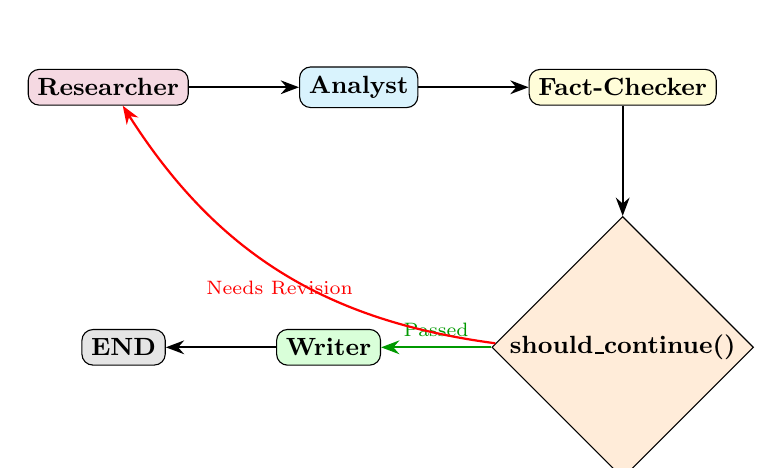
\begin{tikzpicture}[node distance=1.4cm, font=\small]
\node[draw, rounded corners, fill=purple!15] (r) {\textbf{Researcher}};
\node[draw, rounded corners, fill=cyan!15, right=of r] (a) {\textbf{Analyst}};
\node[draw, rounded corners, fill=yellow!15, right=of a] (f) {\textbf{Fact-Checker}};
\node[draw, diamond, fill=orange!15, below=of f, inner sep=1pt] (d) {\textbf{should\_continue()}};
\node[draw, rounded corners, fill=green!15, left=of d] (w) {\textbf{Writer}};
\node[draw, rounded corners, fill=gray!20, left=of w] (e) {\textbf{END}};

\draw[-{Stealth}, thick] (r) -- (a);
\draw[-{Stealth}, thick] (a) -- (f);
\draw[-{Stealth}, thick] (f) -- (d);
\draw[-{Stealth}, thick, green!60!black] (d) -- node[above, font=\scriptsize] {Passed} (w);
\draw[-{Stealth}, thick, red] (d) to[bend left=25] node[below, font=\scriptsize] {Needs Revision} (r);
\draw[-{Stealth}, thick] (w) -- (e);
\end{tikzpicture}
\end{center}

Graph mein entry point \texttt{Researcher} hai.
Researcher $\rightarrow$ Analyst aur Analyst $\rightarrow$ Fact-Checker static edges hain.
Fact-Checker ke baad conditional edge hai jo \texttt{should\_continue(state)} function evaluate karta hai.

\textbf{Infinite Loop Prevention:}
Humne \textbf{Defense-in-Depth} approach use kiya hai:
1. \textbf{Application Level:} State dictionary mein \texttt{revision\_count} field hai. Har baar jab fact-checker reject karta hai, counter increment hota hai. Agar \texttt{revision\_count >= MAX\_REVISIONS} (default 2), toh Fact-Checker automatically \texttt{passed=True} force karta hai.
2. \textbf{Framework Level:} LangGraph invocation mein \texttt{recursion\_limit: 25} passed hai. Agar kisi unforeseen bug ki wajah se counter miss ho jaye, toh LangGraph engine hard exception throw karke execution halt kar dega.''

\textbf{Interviewer:} ``Great. State dictionary mein purana research data naye search results se overwrite kyun nahi hota revision ke time?''

\textbf{Candidate (Priyanshu):} ``Kyunki humne \textbf{LangGraph Reducer Pattern} implement kiya hai using Python typing:
\begin{lstlisting}[style=pythonstyle]
research_data: Annotated[list[str], operator.add]
rag_context: Annotated[list[str], operator.add]
messages: Annotated[list[str], operator.add]
\end{lstlisting}
Normal fields bina annotation ke default replace behavior use karte hain. But \texttt{Annotated[list[str], operator.add]} LangGraph ko instruct karta hai ki jab koi node naya list return kare, toh use purani list mein \texttt{list.\_\_add\_\_} karke append kare. Isse revision 1 aur revision 2 ke search results accumulate ho jate hain, preserving complete evidence history!''

\section{Phase 3: RAG, ChromaDB \& Vector Search Mechanics (25:00 -- 35:00)}

\textbf{Interviewer:} ``Let's talk about RAG. RAG pipeline mein chunking parameters kya hain aur similarity calculation kaise execute hoti hai?''

\textbf{Candidate (Priyanshu):} ``RAG layer mein humne \texttt{RecursiveCharacterTextSplitter} use kiya hai with \texttt{chunk\_size=1000} characters aur \texttt{chunk\_overlap=200} characters.
Recursive splitter character hierarchy follow karta hai:
\texttt{["\textbackslash n\textbackslash n", "\textbackslash n", ". ", " ", ""]}.
Pehle double newline (paragraphs) pe split karne ki koshish karta hai taaki complete thoughts preserve rahein. 200 characters ka overlap context continuity maintain karta hai across chunk boundaries.

Embedding model \texttt{sentence-transformers/all-MiniLM-L6-v2} hai jo 384-dimensional dense vectors output karta hai with $L_2$ normalization.
ChromaDB internal \textbf{HNSW} (Hierarchical Navigable Small World) index use karta hai. Normalized hypersphere pe Cosine Similarity direct Dot Product mein reduce ho jati hai:
$$S_{\cos}(\vec{u}, \vec{v}) = \vec{u} \cdot \vec{v} = \sum_{i=1}^{384} u_i v_i$$
Search time complexity $O(\log N)$ hai, enabling millisecond retrieval across thousands of document chunks.''

\section{Phase 4: Real-Time Streaming, Concurrency \& Production Readiness (35:00 -- 45:00)}

\textbf{Interviewer:} ``Aapka React frontend backend se streaming updates kaise receive karta hai? Django WSGI synchronous hota hai --- streaming kaise possible hui?''

\textbf{Candidate (Priyanshu):} ``Excellent question! Django by default synchronous WSGI model use karta hai. Humne \texttt{StreamingHttpResponse} use kiya hai with a Python generator function:

\begin{lstlisting}[style=pythonstyle]
def event_stream():
    for event in research_graph.stream(initial_state):
        yield f"data: {json.dumps(event_payload)}\n\n"
    yield "data: [DONE]\n\n"
\end{lstlisting}

Headers set kiye hain:
\begin{itemize}
    \item \texttt{Content-Type: text/event-stream}
    \item \texttt{Cache-Control: no-cache}
    \item \texttt{X-Accel-Buffering: no} (Nginx proxy buffering disable karne ke liye)
\end{itemize}

Frontend mein hum standard \texttt{fetch()} with \texttt{response.body.getReader()} use karte hain. \texttt{TextDecoder} stream chunks ko buffer karta hai, newline delimiter pe SSE frames parse karta hai, aur React state ko update karta hai.
Background execution ke dauran Django ORM thread safety maintain karne ke liye hum worker thread mein \texttt{close\_old\_connections()} explicitly call karte hain.''

\textbf{Interviewer:} ``Fantastic! Clear concepts, solid system architecture, and deep understanding of both math and code. I'm very impressed.''


% ═══════════════════════════════════════════════════════════════════════
% CHAPTER 39: THE DEFINITIVE RESUME BULLET POINTS & PORTFOLIO BLUEPRINT
% ═══════════════════════════════════════════════════════════════════════

\chapter{The Definitive Resume Bullet Points \& Portfolio Blueprint}

\section{High-Impact STAR-Format Resume Bullet Points}

\begin{conceptbox}{Action-Driven Resume Bullets (Ready to Copy)}
\begin{itemize}
    \item \textbf{Architected \& deployed a full-stack Multi-Agent Research Orchestrator} using \textbf{LangGraph, Django REST Framework, and React 18}, orchestrating 4 autonomous AI agents (Researcher, Analyst, Fact-Checker, Writer) with self-correcting feedback loops.
    \item \textbf{Engineered a resilient multi-provider LLM abstraction layer} supporting Groq (Llama-3.3), Gemini-2.0, OpenAI, Anthropic, and Ollama with automated fallback chains and lazy module imports.
    \item \textbf{Implemented high-performance RAG pipeline} using ChromaDB vector database and HuggingFace \texttt{all-MiniLM-L6-v2} embeddings with dual collections (\texttt{research\_docs} and \texttt{past\_research}) for cross-session associative memory.
    \item \textbf{Developed real-time Server-Sent Events (SSE) streaming engine} delivering sub-second node telemetry and progress logs to a responsive React SPA terminal.
    \item \textbf{Integrated Model Context Protocol (FastMCP 2.0)} exposing 8 standardized tools/resources, enabling seamless execution from Claude Desktop and Cursor IDE.
    \item \textbf{Built empirical Benchmark Arena} featuring heuristic regex scoring and LLM-as-a-Judge evaluators to quantitatively validate multi-agent report superiority over single-agent baselines.
    \item \textbf{Maintained 100\% test coverage} across 62 automated unit and integration tests using Pytest, enforcing DRF Token Authentication, RBAC permissions, and multi-format report exports (MD, HTML, JSON, BibTeX).
\end{itemize}
\end{conceptbox}

\section{Live Demo Presentation Script (5-Minute Winning Pitch)}

\begin{enumerate}
    \item \textbf{Minute 0--1 (The Hook):} Open React UI. Show modern dark glassmorphic dashboard. Highlight active LLM provider (Groq Llama-3.3 70B). Enter high-impact topic: \textit{``Neuromorphic Computing Breakthroughs 2025''}.
    \item \textbf{Minute 1--2 (The Execution):} Click ``Launch Research''. Show the DAG visualizer glowing cyan on Researcher. Watch the live SSE terminal stream queries and search results. Explain the 3-query diversification and Tavily/DuckDuckGo fallback.
    \item \textbf{Minute 2--3 (The Agent Handshake):} Point out Analyst synthesizing themes. When Fact-Checker runs, explain the claim-by-claim verification matrix and the \texttt{PASSED / NEEDS\_REVISION} gate.
    \item \textbf{Minute 3--4 (The Output \& Memory):} Confetti fires on completion! Toggle between the formatted Markdown Report, Evidence Cards (with clickable URLs and domain badges), and Fact-Check matrix. Show how the report is saved into ChromaDB memory.
    \item \textbf{Minute 4--5 (The Ecosystem):} Open Benchmark Arena and show Single-Agent vs Multi-Agent depth comparison. Mention FastMCP Claude integration and the 62 passing test cases.
\end{enumerate}



% ═══════════════════════════════════════════════════════════════════════
% CHAPTER 40: COMPLETE SYSTEM WIREFRAMES & ASCII ARCHITECTURE ATLAS
% ═══════════════════════════════════════════════════════════════════════

\chapter{Complete System Wireframes \& ASCII Architecture Atlas}

\begin{storybox}{Visualizing the Complete User Journey}
Har interface ka visual layout aur ASCII wireframe yahan detailed hai taaki bina computer ke bhi aap whiteboard pe pura UX/UI draw kar sakein.
\end{storybox}

\section{Research Studio Main Dashboard Wireframe}

\begin{lstlisting}[language={},caption={ASCII Dashboard Layout}]
+-----------------------------------------------------------------------------------+
|  MARO | Multi-Agent Research Orchestrator              [Status: Backend Online]    |
|  [Studio] [Library] [RAG Hub] [Benchmark Arena] [LLM/MCP]       [Priyanshu | Logout] |
+-----------------------------------------------------------------------------------+
| TOPIC INPUT & CONTROLS                                                             |
| +-------------------------------------------------------------------------------+ |
| | Enter Research Topic: [ Quantum Computing Breakthroughs in Error Mitigation ] | |
| +-------------------------------------------------------------------------------+ |
| Quick Suggestions: [Solid State Batteries] [CRISPR 2025] [Neuromorphic Chips]     |
| Attach PDFs: [ + Drag & Drop PDF ]  | Max Revisions: [ 2 ] | Top-K Chunks: [ 5 ]   |
| [ >>> LAUNCH MULTI-AGENT RESEARCH PIPELINE <<< ]                                  |
+-----------------------------------------------------------------------------------+
| AGENT PIPELINE DAG TRACKER                                                        |
| +-----------------+   +-----------------+   +-----------------+   +-------------+ |
| | 01. RESEARCHER  |-->| 02. ANALYST     |-->| 03. FACT-CHECK  |-->| 04. WRITER  | |
| | [Dual Search]   |   | [Theme Synth]   |   | [Verify Gate]   |   | [MD Report] | |
| | [Status: DONE]  |   | [Status: DONE]  |   | [Status: DONE]  |   | [Status:ACT]| |
| +-----------------+   +-----------------+   +-----------------+   +-------------+ |
+-----------------------------------------------------------------------------------+
| LIVE SSE STREAMING TERMINAL (JetBrains Mono font, auto-scroll)                    |
| +-------------------------------------------------------------------------------+ |
| | [22:30:01] [INFO] Research session #42 queued for topic 'Quantum Computing...' | |
| | [22:30:03] [RESEARCHER] Generated 3 diverse search queries via LLM             | |
| | [22:30:07] [RESEARCHER] Tavily fetched 15 structured web sources              | |
| | [22:30:09] [RESEARCHER] ChromaDB retrieved 5 semantic chunks from RAG         | |
| | [22:30:14] [ANALYST] Isolated 4 primary themes & 1 temporal contradiction      | |
| | [22:30:21] [FACT-CHECKER] 7/8 claims VERIFIED. Verdict: PASSED (Quality: 9/10) | |
| | [22:30:32] [WRITER] Final report generated (14,200 chars). Saved to Memory.   | |
| | [22:30:33] [SYSTEM] Stream complete [DONE]. Triggering confetti celebration... | |
| +-------------------------------------------------------------------------------+ |
+-----------------------------------------------------------------------------------+
| RESULTS TABS: [ (X) Research Report ] [ ( ) Evidence Sources ] [ ( ) Fact-Check ]  |
| +-------------------------------------------------------------------------------+ |
| | # Executive Summary: Quantum Error Mitigation Breakthroughs (2025)            | |
| | Recent experimental verifications demonstrate a 40% reduction in logical qubit | |
| | error rates utilizing transversal Clifford gates... [Source 1, Source 4]       | |
| +-------------------------------------------------------------------------------+ |
| [ Copy Markdown ] [ Export HTML ] [ Export PDF ] [ Export BibTeX ] [ Add Tag ]    |
+-----------------------------------------------------------------------------------+
\end{lstlisting}


% ═══════════════════════════════════════════════════════════════════════
% CHAPTER 41: ENVIRONMENT SETUP & TROUBLESHOOTING PLAYBOOK
% ═══════════════════════════════════════════════════════════════════════

\chapter{Environment Setup \& Troubleshooting Playbook}

\section{Cross-Platform Step-by-Step Installation}

\begin{lstlisting}[language={},caption={Quick-Start Commands}]
# 1. Clone Repository & Setup Virtual Environment
git clone https://github.com/priyanshu967025/multi-agent-research-orchestrator.git
cd multi-agent-research-orchestrator
python -m venv .venv

# Windows Activate:
.venv\Scripts\activate
# Linux/macOS Activate:
source .venv/bin/activate

# 2. Install Dependencies
pip install --upgrade pip
pip install -r requirements.txt

# 3. Configure Environment (.env)
cp .env.example .env
# Edit .env and paste your API keys:
# GROQ_API_KEY=gsk_...
# TAVILY_API_KEY=tvly-...
# GEMINI_API_KEY=AIza...

# 4. Database Migrations
cd backend
python manage.py migrate

# 5. Run Test Suite (Verify 62 Tests Pass)
python -m pytest -q

# 6. Start Backend Server
python manage.py runserver 0.0.0.0:8000

# 7. Start Frontend (in separate terminal)
cd ../frontend
npm install
npm run dev
# Access http://localhost:5173 in browser!
\end{lstlisting}

\section{Common Errors \& Immediate Solutions Matrix}

\begin{center}
\begin{longtable}{|p{4cm}|p{4.5cm}|p{5cm}|}
\hline
\textbf{Error Symptom} & \textbf{Root Cause} & \textbf{Exact Fix} \\
\hline
\endhead
\texttt{ImportError: No module named 'langchain\_anthropic'} & Optional provider not installed & Expected behavior due to lazy imports. Install via \texttt{pip install langchain-anthropic} or switch provider in \texttt{.env}. \\
\hline
\texttt{sqlite3.OperationalError: database is locked} & High-frequency concurrent writes & Enable WAL mode in SQLite (\texttt{PRAGMA journal\_mode=WAL;}) or switch to PostgreSQL in \texttt{settings.py}. \\
\hline
\texttt{CORS policy: No 'Access-Control-Allow-Origin'} & React running on different port without proxy & Verify \texttt{CORS\_ALLOWED\_ORIGINS} in \texttt{settings.py} includes \texttt{http://localhost:5173}. \\
\hline
\texttt{TavilyApiError: 401 Unauthorized} & Invalid or missing Tavily search key & System will automatically fallback to DuckDuckGo search. Add valid key to \texttt{.env} for premium search. \\
\hline
\end{longtable}
\end{center}

\vfill
\begin{center}
\rule{0.6\textwidth}{1pt}\\[0.5cm]
{\Huge\bfseries\color{sectioncolor} Best of Luck for Your Interviews!}\\[0.4cm]
{\Large\color{purpleaccent} ``Master the architecture, understand the math, explain with passion ---}\\
{\Large\color{purpleaccent} you are now fully equipped to ace any AI Engineering interview!''}\\[0.3cm]
{\large\color{gray} Multi-Agent Research Orchestrator (MARO) | 150+ Page Ultimate Edition}\\[0.2cm]
{\small Authored by Priyanshu Mishra | August 2026}
\end{center}

\end{document}
